
%\documentclass[german,reviews,examples]{isasthesis}
\documentclass[english,reviews,examples]{isasthesis}

\usepackage[utf8]{inputenc}
% \usepackage{footbib}
\usepackage{graphicx}
\usepackage{float}
\usepackage{amsmath}
\usepackage{amssymb}
\usepackage{booktabs}
\usepackage{setspace}
\usepackage{placeins}
\usepackage[binary-units]{siunitx} %For the SI notation in Chap. 4
\usepackage{multirow} %for tables
\usepackage{dirtytalk}%for quotation
\usepackage{csquotes}%also for quotation
\usepackage{supertabular}%for long tabular
\usepackage{svg}
% \usepackage[T1]{fontenc}%italic in title
\usepackage[toc,page]{appendix}

% \usepackage{algorithmicx}
% \usepackage{algpseudocode}
\graphicspath{{figures/}}

\usepackage[style=ieee-alphabetic, sorting=none, backend=bibtex]{biblatex}
\addbibresource{ref.bib}

%%%%%%%%%%%%%%%%%%%%%%%%%%%%%%%%%%
% Edit notation.tex if necessary
%%%%%%%%%%%%%%%%%%%%%%%%%%%%%%%%%%

%%%%%%%%%%%%%%%%%%%%%%%%
% Document properties
%%%%%%%%%%%%%%%%%%%%%%%%

\title{Sensitivity Analysis of a Multitarget Tracker with \\Machine Learning and Data Analysis Methods}
\author{Weining Ye}
% {31. Dezember 2020}
\date{\today}

\thesistype{Master's Thesis}
\discussant{Prof. Dr.-Ing. Thomas Längle}
\firstsupervisor{M.Sc. Marcel Reith-Braun}
\secondsupervisor{Dr.-Ing. Florian Pfaff}

%%%%%%%%%%%%%%%%%%%%%%%%
% Document
%%%%%%%%%%%%%%%%%%%%%%%%

\begin{document}
    \maketitle

    
\renewcommand{\abstractname}{Abstract}
\begin{abstract}
The multitarget tracking algorithm in optical belt sorting needs different hyperparameters that are vital for the accuracy of the tracking. The values of the hyperparameters are highly dependent upon the characteristics of the tracked objects and the setting of the experiments, such as the shape, size and density of the particles. However, these hyperparameters have been manually determined until now.

The multitarget tracking algorithm consists of two parts: single target motion prediction and association. We present methods for finding values of the hyperparameters that reduce the errors in both parts in this thesis. For prediction hyperparameters, grid search is first used for showing the general effect of the hyperparameters. Then the Bayesian optimization method is validated with an artificial dataset. Finally, Bayesian optimization is performed to optimize the hyperparameters with real-world measurements of different materials. We can observe a significant enhancement of the prediction accuracy with optimized hyperparameters compared to default hyperparameters. We also discuss the difference of the optimized hyperparameter value between materials. The results show that the different material types and sizes of the particle can have an effect on the optimized value of hyperparameters.

In the part of association hyperparameters, the concept of the robust range is first introduced, which indicates the range of hyperparameters that ensures no association errors. Then the general effect of the association hyperparameters is examined with grid search. Finally, the SVMs are trained to represent the robust range. The determination criteria for the robust range based on the average prediction error and particle density are also discussed, and the hyperparameters calculated from the criteria are checked with more datasets.
\end{abstract}





    \maketoc
    
    \chapter{Introduction}
% First chapter.
% \section{Background}

Belt sorting is a type of technology that can automatically separate different types of materials or filter out the unaccepted products from the material flow with conveyor belts. This technology has been widely used in different industry areas, such as mining, recycling \cite{pfaff2015tracksort} and food processing \cite{edwards2004detecting}. Belt sorting enables an automatic process of sorting that significantly saves time, human resources, cost as well as energy \cite{zsifkovits2020state}.

Optical sorting sorts bulk materials according to the optical features of the particles. Compared with the other sorting methods based on the physical properties, optical sorting is less limited from the type of materials and able to sort the materials in a non-destructive way. An optical belt sorting system usually comprises four parts: the feed system, the optical system, the data processing system, and the separation system, as illustrated in Figure \ref{belt sort system old} \cite{edwards2004detecting}. Conventional optical belt sorting systems use a line camera at the end of the conveyor belt to detect the particles. In this case, each particle is observed only once and assumed as flying straightly in the transport direction and reaching the separator after a fixed delay \cite{wotruba2008stand}. However, this simple motion model is inadequate for predicting the motion of the particles, and the sorting accuracy is therefore limited, as shown in Figure \ref{line camera error}.

\begin{figure}[htb]
\centering
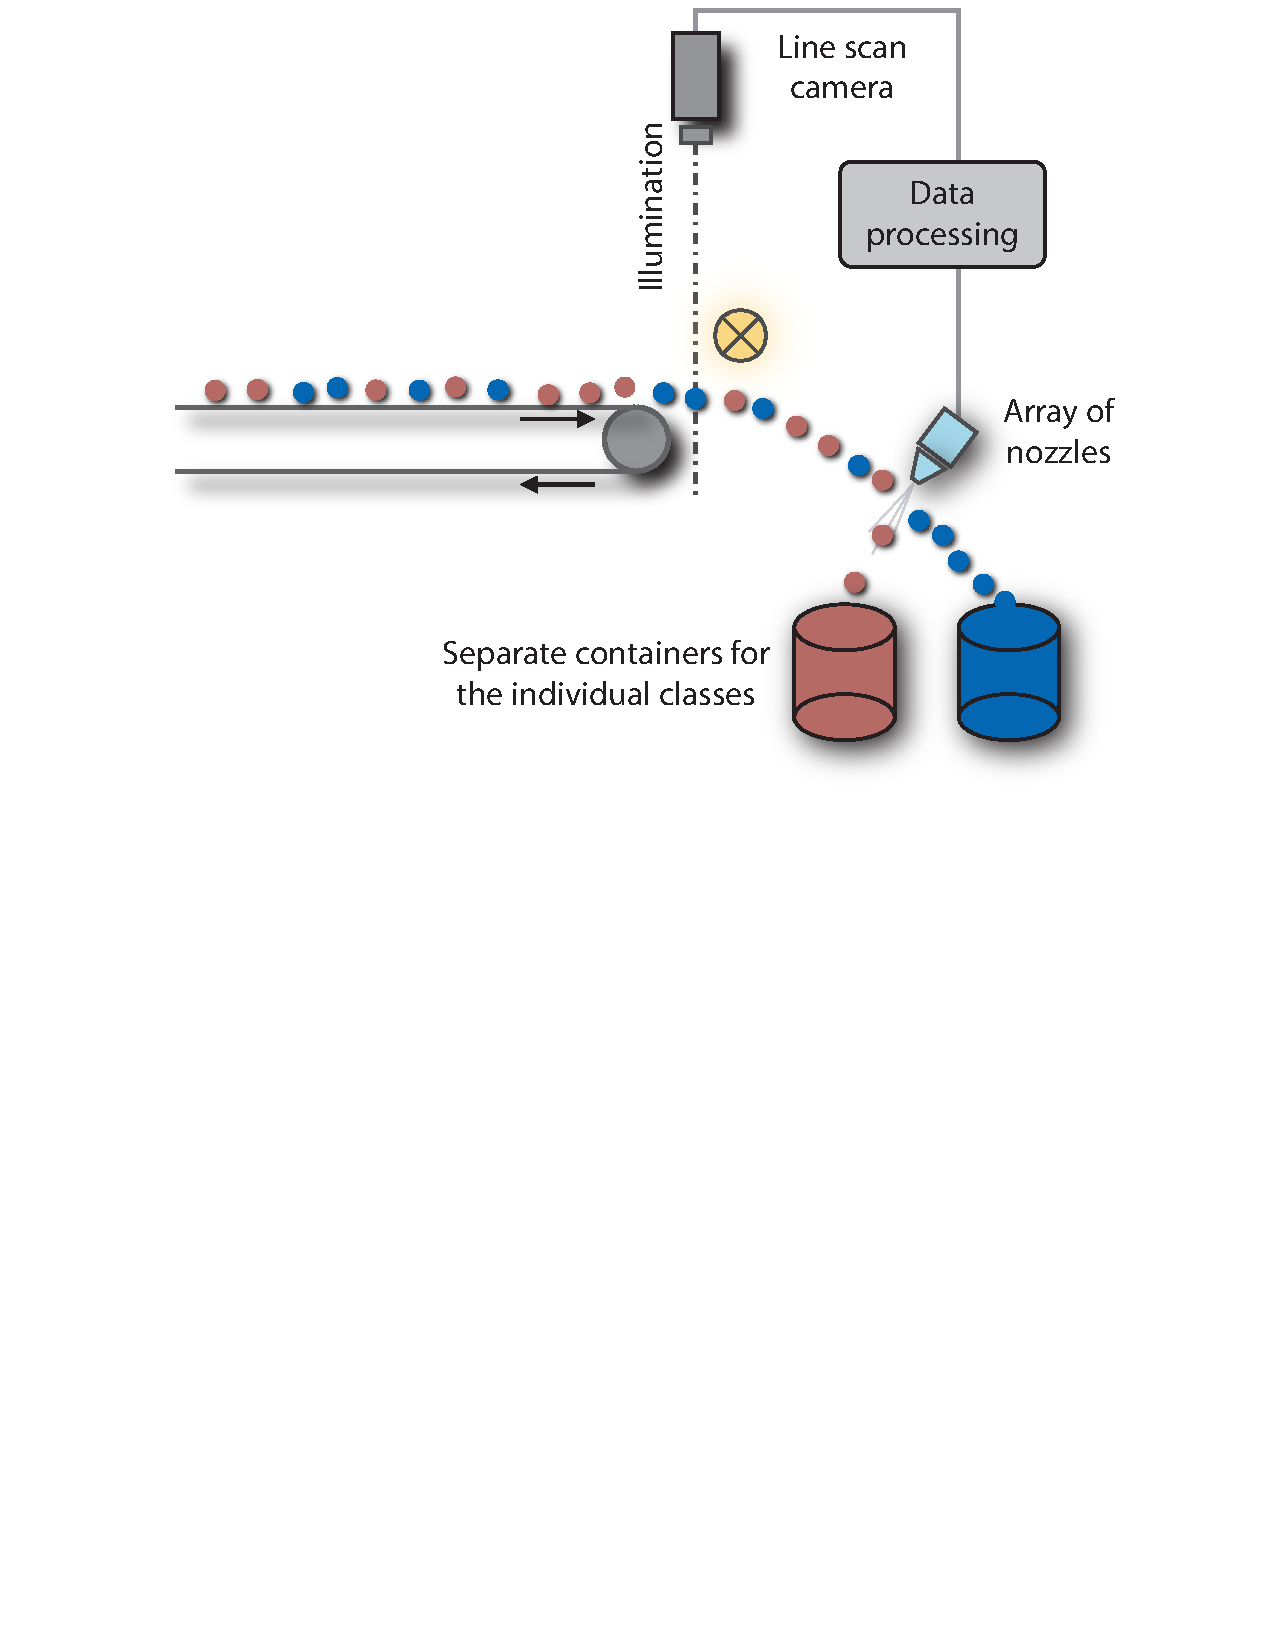
\includegraphics[width=0.5\textwidth]{figures/sort system old.pdf}
\caption{Structure of a conventional optical belt sorting system with line scan camera. In our recent research, the line scan camera has been replaced with a area scan camera. The figure is adapted from \cite{pfaff2017improving}.}
\label{belt sort system old}
\end{figure}

\begin{figure}[htb]
\centering
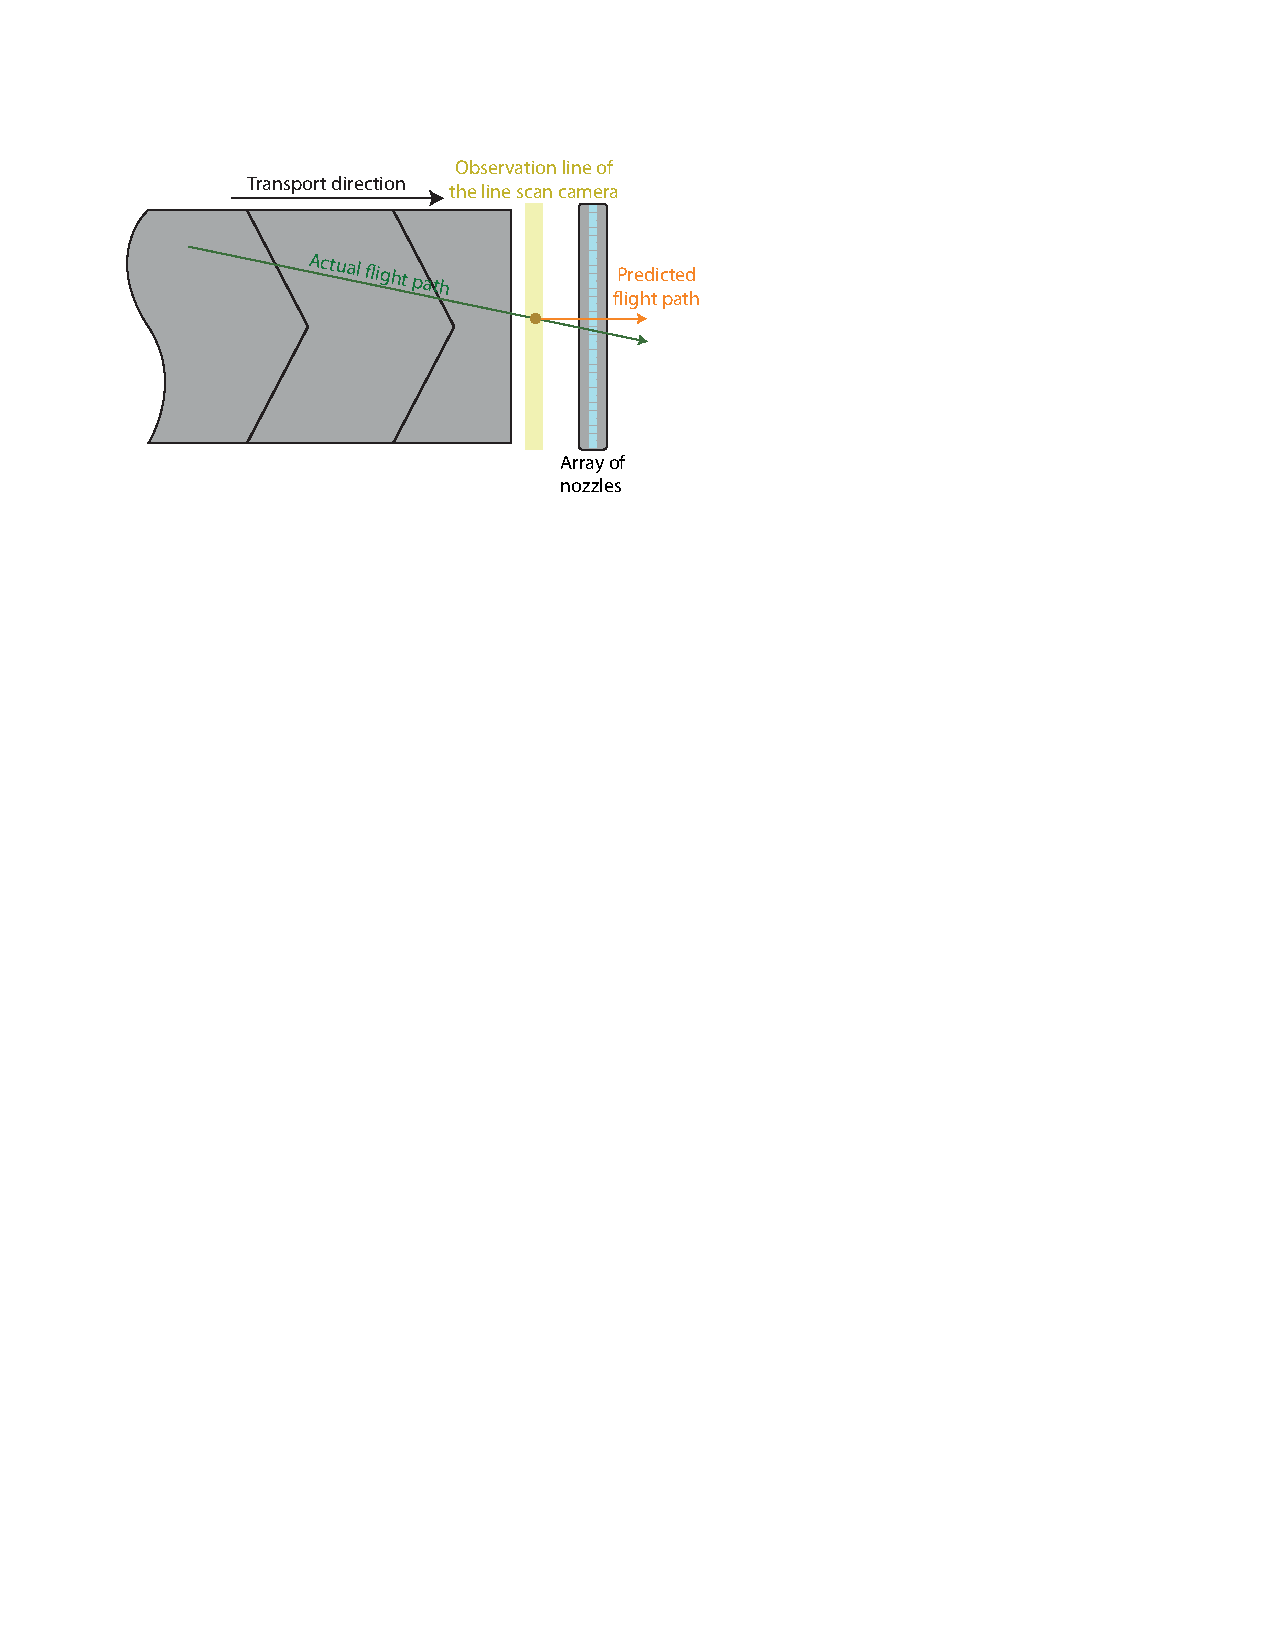
\includegraphics[width=0.5\textwidth]{figures/line camera.pdf}
\caption{Illustration that the prediction of the particle motion can be imprecise when assuming a motion straight along the transport direction \cite{pfaff2019multitarget}.}
\label{line camera error}
\end{figure}

In order to overcome the drawbacks of the belt sorter with line cameras, Pfaff et al. \cite{pfaff2019multitarget} replaced the line cameras with area cameras. The area camera takes pictures containing multiple particles, and the particles can be observed from the camera in multiple frames. With the area camera, we are able to perform a multitarget tracking of the particles on the belt, with which the more precise information of the particles, such as velocity and even acceleration, can be obtained. Then with the motion model for the prediction to the separator nozzles, the motion of the particles can be more accurately predicted.

\section{Motivation and Contribution}

The multitarget tracking algorithm is composed of the single-target motion prediction part that estimates the motion of particles and the association part that assigns the measurements to each particle, as shown in Figure \ref{tracking system simple}. In both parts, the algorithm needs different hyperparameters that need to be tuned before we are able to run the algorithm properly, such as the variance term in Kalman filter and the penalty term in the association matrix. Choosing appropriate parameters for different bulk materials can significantly improve the performance of the multitarget tracking algorithm.

\begin{figure}[htb]
\centering
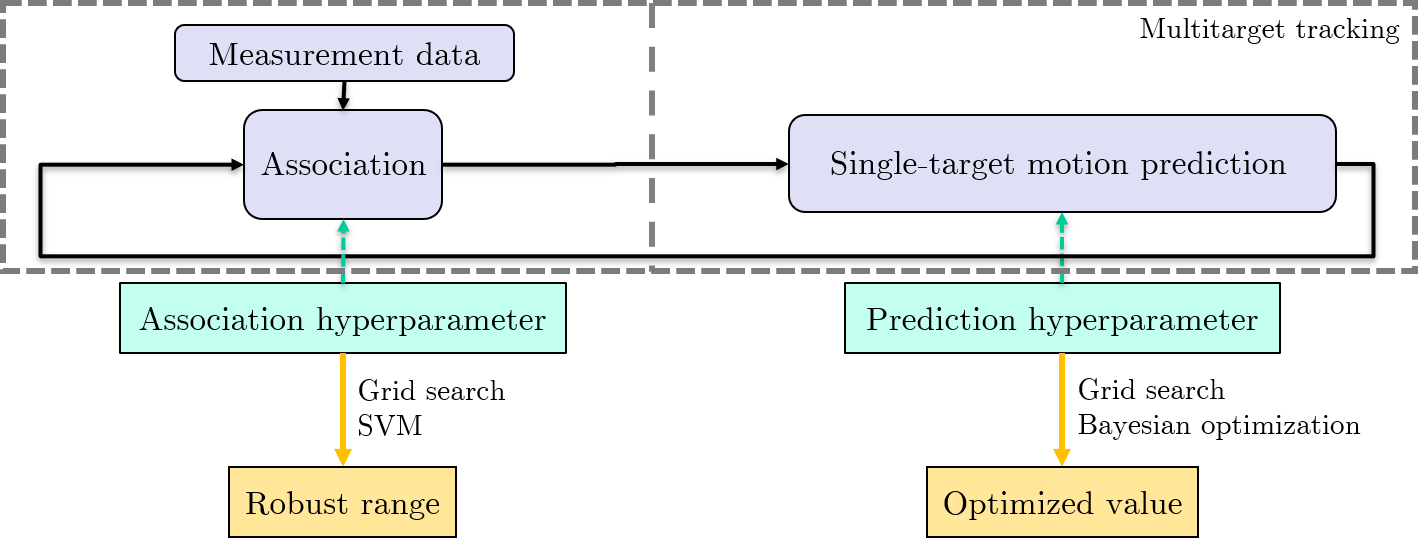
\includegraphics[width=0.9\textwidth]{figures/tracking system simple.png}
\caption{Structure of the multitarget tracking algorithm, including the single-target motion prediction part and the association part, which contain different hyperparameters. These hyperparameters are optimized with different methods in this thesis.}
\label{tracking system simple}
\end{figure}

The optimal value of the hyperparameters depend on many properties of the material, such as the shapes and sizes of the particles. However, the hyperparameters have been manually determined so far and lack a systematic method for finding the optimal values. These manually determined values of hyperparameters are not adaptive to the different materials or dynamical situations in sorting. Therefore, the hyperparameters need to be optimized, and the optimization methods should be generalized for all kinds of materials.


In this thesis, the hyperparameters in both parts of the tracking algorithm are optimized with different methods. In the single-target motion prediction part, the hyperparameters are optimized with grid search and Bayesian optimization. The prediction error is lowered with the optimized hyperparameters, and the difference of the optimized hyperparameter values between materials is discussed. The robust ranges of the association hyperparameters are determined with grid search and SVMs. The determination criteria for the robust range based on the average prediction error and particle density are also discussed.

\section{Thesis Outline}


In Chapter 2, we introduce the theoretical basis needed in this thesis, including the basic ideas of the tracking algorithm and optimization algorithms. These contents can give us the initial knowledge of the multitarget tracking system we work on and the optimization tools we have. Chapter 3 presents more details of the implementation of the multitarget tracking algorithm. All the hyperparameters for the optimization are also listed in this chapter. Chapter 4 makes an introduction of the datasets used in the thesis. Chapter 5 introduces the method and their settings for the optimization works in this thesis. The evaluation criteria of the prediction and association performance is also presented in this chapter. Chapter 6 shows the results of all experiments, including the optimized values for hyperparameters and the effect of optimizations. Some explanations and discussions are also given after the results. The thesis ends with Chapter 7, which gives the conclusion of this thesis as well as some suggestions and outlooks for future researches.




% s. The first half of this chapter presents the initial knowledge of the tracking algorithm, including the system model, Kalman filter, motion models and multitarget tracking. The important algorithms for optimization and classification are reviewed in the second half of this chapter. The optimization algorithms are explained briefly in Section 2.3. Then the method of grid search and Bayesian optimization is in detail explained. In Section 2.4, the principle of SVM is explained. In the following section, overfitting and the methods for avoiding it are discussed.

% Chapter 3 presents more detailed knowledge of the \textit{TrackSort} algorithm. In the first two sections, the basics of the traditional belt sorting system as well as the development of the \textit{TableSort}-System and the \textit{TrackSort} algorithm are presented. In Section 3.3, the \textit{TrackSort} algorithm is more in detail explained, including the motion models used for tracking and the methods for data association and track management.

% Chapter 4 focuses on the datasets used in the thesis. Four types of datasets are introduced, namely the datasets from single real materials, the datasets from mixed real materials, the DEM datasets and the artificial datasets.

% Chapter 5 introduces the method for the optimization works in this thesis. In Section 5.1, the evaluation metrics for motion prediction and association are first presented. Then in Section 5.2 the methods and settings for optimization of the prediction hyperparameters are depicted. In Section 5.3, the concept of the robust range is introduced, then the settings and the process of the training of SVMs are in detail explained.

% Chapter 6 shows the results of all experiments. The effect of the prediction hyperparameters is shown in Section 6.1, then the optimized value for the test dataset and more datasets are presented in the following subsections. In Section 6.2, the result of the robust range for association hyperparameters is explained.

% The thesis ends with Chapter 7, which gives the conclusion of this thesis. In this chapter, some suggestions and outlooks for future research are also raised.
    \chapter{Theoretical Basics}

This chapter introduces the theoretical basis needed in this thesis. The first half of this chapter presents the initial knowledge of the tracking algorithm, including the general dynamic system model, Kalman filter, motion models and multitarget tracking. The important algorithms for optimization and classification are reviewed in the second half of this chapter. The optimization algorithms are explained briefly at the start of Section 2.3. Then the method of grid search and Bayesian optimization is in detail explained. In Section 2.4, the principle of SVM is explained. In the following section, overfitting and the methods for avoiding it are discussed.

\section{Single-Target Tracking}
\label{st}

% \textcolor{red}{(of course we need tracking) what is the tracking process(estimation of a dynamic system) - what is the estimation - introduce single target tracking because it's the simplest tracking system and the basis of MTT. }

% \textcolor{red}{Then in subsection: 1. the dynamic system (needed for tracking process) 2. estimation with KF(estimation) 3. motion model}


The tracking process can be recognized as a state estimation problem of a dynamic system. The simplest dynamic system in the tracking problem is the single-target tracking (STT) system that assumes only one target at the same time in the area of interest. The STT is also the basis for the multitarget tracking.

\subsection{Dynamic System Model}

A typical time-discrete dynamic system can be represented by functions between random variables. The random state vector $\boldsymbol{\underline{x}}_{t}$ is a function of the random state in the last timestep $\boldsymbol{\underline{x}}_{t-1}$, the external input $\hat{\underline{u}}_{t-1}$ and the random system noise $\boldsymbol{\underline{w}}_{t-1}$ with a given distribution \cite{welch1995introduction}.  Therefore, the state transition function $a_{t}$  can be represented with the function

\begin{equation}
    \boldsymbol{\underline{x}}_{t+1} = a_{t}(\boldsymbol{\underline{x}}_{t},\,\hat{\underline{u}}_{t},\,\boldsymbol{\underline{w}}_{t}).
\end{equation}

The measurement $\boldsymbol{\underline{z}}_{t}$ is a function of the state of the tracked object $\boldsymbol{\underline{x}}_{t}$ and the random measurement noise $\boldsymbol{\underline{v}}_{t}$ with a given distribution \cite{welch1995introduction}. Therefore, the measurement function $h_{t}$ can be represented with the function

\begin{equation}
    \boldsymbol{\underline{z}}_{t} = h_{t}(\boldsymbol{\underline{x}}_{t},\,\boldsymbol{\underline{v}}_{t}).
\end{equation}

In this thesis, the tracking problem was assumed as with a linear time-invariant (LTI) system that follows the linear state transition model. Further, the motion model and noise in the tracking process are assumed to be identical for all time steps and all objects, hence the time index of the system matrices can be neglected. The system has also no external input. Therefore, the state transition model can be represented with these two functions

\begin{gather}
    \boldsymbol{\underline{x}}_{t+1}^{\mathrm{Lin}} = \mathbf{F}\boldsymbol{\underline{x}}_{t}^{\mathrm{Lin}}+\boldsymbol{\underline{w}}\\
    \boldsymbol{\underline{z}}_{t}^{\mathrm{Lin}} = \mathbf{H}\boldsymbol{\underline{x}}_{t}^{\mathrm{Lin}}+\boldsymbol{\underline{v}}.
\end{gather}

In these two functions, the matrix $\mathbf{F}$ contains the information of the state transition model. The matrix $\mathbf{H}$ contains the information of the measurement system. The vector $\boldsymbol{\underline{w}}$ and $\boldsymbol{\underline{v}}$ represent respectively the system and measurement noise.


\subsection{Kalman Filter}
\label{kf}

Estimation is defined as the process of inferring the value of a quantity from indirect and uncertain observations. Filtering is the estimation of the state of a dynamic system from noisy observations amounts by ``filtering out" the noise \cite{bar2004estimation}. The Kalman filter is the most prevalent method for solving linear tracking problems having independent Gaussian random errors with zero mean \cite{stone2013bayesian}. It provides an efficient computational means to estimate the state of a process, in a way that minimizes the mean of the squared error between the estimation and the real state of the system  \cite{maybeck1982stochastic}. 

The Kalman filter estimates the state of a dynamic system by using a form of feedback control: the filter estimates the system state at the next timestep and then obtains feedback in the form of noisy measurements. As such, the algorithm for the Kalman filter can be divided into two parts: prediction step and update step, as depicted in Figure \ref{Structure Kalman filter}. 

\begin{figure}[htbp]
\centering
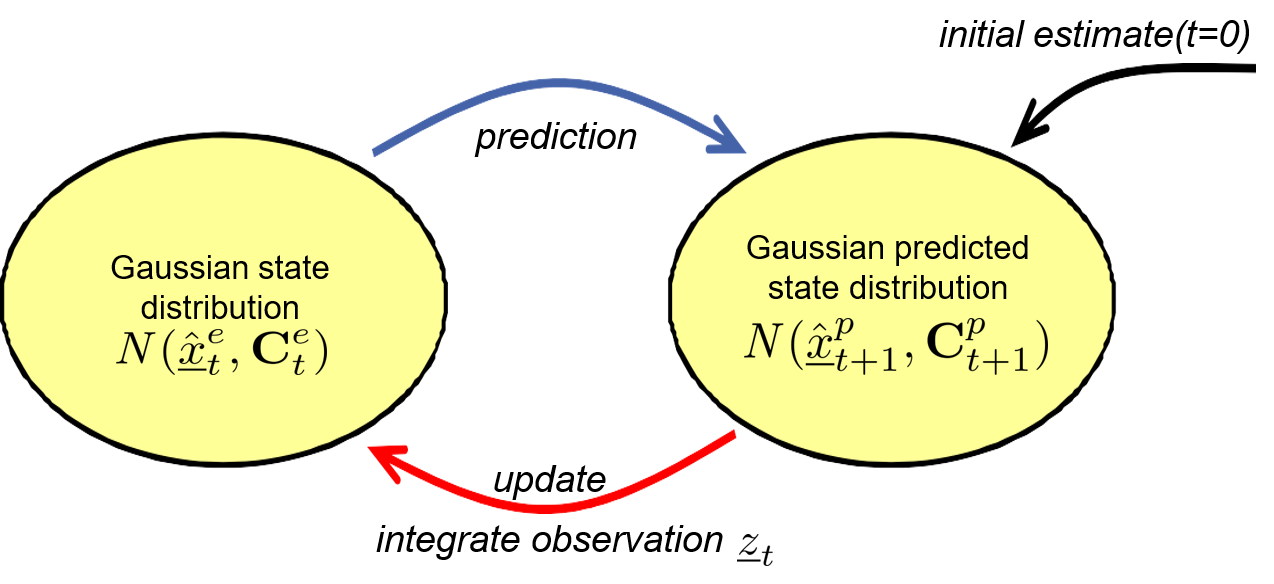
\includegraphics[width=0.8\textwidth]{figures/Structure Kalman Filter2.png}
\caption{The cycle of the recursive Kalman filter. The prediction process generates the state estimation with the estimated state from the last timestep and the given motion model. The update process updates the system state on the base of measurements  \cite{welch1995introduction}.}
\label{Structure Kalman filter}
\end{figure}

The equations in the prediction step are responsible for predicting the state $\hat{\underline{x}}^{\mathrm{p}}_{t+1}$ and the error covariance $\textbf{C}_{t+1}^{\mathrm{p}}$ to obtain the \textit{a priori} estimation for the next time step. The equations for the prediction step are presented as 
\begin{gather}
    \hat{\underline{x}}^{\mathrm{p}}_{t+1}=\mathbf{F}\hat{\underline{x}}^{\mathrm{e}}_{t}\\
    \mathbf{C}_{t+1}^{\mathrm{p}}=\mathbf{F}\mathbf{C}_{t}^{\mathrm{e}}\mathbf{F}^\top+{ \mathbf{C}_{t}^{\underline{\boldsymbol{w}}}}, 
\end{gather}

where the matrix $\mathbf{C}_{t}^{\underline{\boldsymbol{w}}}$ represents the system noise that depends on the difference between real system state transition and the predefined system model. The system matrix $\mathbf{F}$ and the system noise matrix $\mathbf{C}_{t}^{\underline{\boldsymbol{w}}}$ contains all the information about the system model required by the Kalman filter \cite{pfaff2019multitarget}.

The update equations are responsible for incorporating the new measurements with the \textit{a priori} estimation to obtain an improved \textit{a posteriori} estimation that contains the estimated state $\hat{\underline{x}}^{\mathrm{e}}_{t}$ and error covariance $\mathbf{C}_{t}^{\mathrm{e}}$. The equations for the update step are presented as
\begin{gather}
    \textbf{K}_{t}=\textbf{C}_{t}^{\mathrm{p}}\mathbf{H}({\textbf{C}_{t}^{\underline{\boldsymbol{v}}}}+\mathbf{H}\textbf{C}_{t}^{\mathrm{p}}\mathbf{H}^\top)^{-1}\\
    \textbf{C}_{t}^{\mathrm{e}}=(1-\textbf{K}_{t}\mathbf{H})\textbf{C}_{t}^{\mathrm{p}}\\
    \hat{\underline{x}}^{\mathrm{e}}_{t}=\hat{\underline{x}}^{\mathrm{p}}_{t}+\textbf{K}_{t}(\hat{\underline{z}}_{t}-\mathbf{H}\hat{\underline{x}}^{\mathrm{p}}_{t}), 
\end{gather}

where the matrix $\mathbf{H}$ contains the information of the measurement system and the matrix $\mathbf{C}_{t}^{\underline{\boldsymbol{v}}}$ represents the measurement noise that depends on the measurement accuracy. With the optimal Kalman gain $\textbf{K}_{t}$, the estimation error $\left \| \hat{\underline{x}}_{t}-\hat{\underline{x}}^{\mathrm{e}}_{t} \right \|$ is minimized \cite{welch1995introduction}.

However, the exact system and measurement covariance matrices are hard to obtain for most of the real systems. As a result, the Kalman filter often works with incorrect noise matrices. The sensitivity analysis describes the sensitivity of the estimation error to incorrectly input noise matrices in the estimator \cite{lu2014false}. In this thesis, the values of these input matrices will be the hyperparameters for the sensitivity analysis and the optimization.



\subsection{Motion and Measurement Model in Tracking}
\label{cv basic}
% \textcolor{red}{This part is changed with 1-D CV model, the 2-D case is moved to chapter 3. Title changed to "motion and measurement model"}
The motion model is the system model for the tracking problem, which describes the motion of the tracked objects in the tracking process. There are many motion models based on different system characteristics, which mainly include the position, velocity and angular velocity of tracked objects \cite{li2003survey}\cite{schubert2008comparison}. 

The constant velocity model is a widely used simple motion model for tracking. In this model, the velocity of tracked objects are considered as constant, and the accelerations are assumed to be zero in noise-free cases. However, the velocity does not remain really ``constant" in the tracking. As a part of the state vector, the value of the velocity can change because of the measurement noise.

Take the 1-D constant velocity model as an example. In the model, the state vector contains the position and velocity of the tracked objects along and vertical to the transport directions \cite{pfaff2019multitarget}
\begin{equation}
    \underline{x}_{t}=
    \begin{bmatrix}
        \mathsf{x}_{t}\\ 
        \dot{\mathsf{x}}_{t}
    \end{bmatrix}.
\end{equation}

The system matrix for the constant velocity model is
\begin{equation}
    \mathbf{F}=\begin{bmatrix}
     1 & T \\ 
     0 & 1
    \end{bmatrix} ,
\end{equation}
with $T$ denoting the time between two subsequent time steps. 

The system noise covariance is given by
\begin{equation}
    \mathbf{C}^{\underline{\boldsymbol{w}}}=S^{\boldsymbol{w}}
    \begin{bmatrix}
     T^3/3 & T^2/2\\ 
     T^2/2 & T 
    \end{bmatrix} ,
\end{equation}
where the $S^{\boldsymbol{w}}$ is the power spectral density of the system noise.

Only the position can be directly observed in the measurement process. Therefore, the measurement matrix is
\begin{equation}
    \mathbf{H}=\begin{bmatrix}
     1 & 0
    \end{bmatrix} .
\end{equation}

The measurement position variance is represented with the measurement noise power spectral density $S^{\boldsymbol{v}}$ in this case, as
\begin{equation}
    \mathbf{C}^{\underline{\boldsymbol{v}}}=S^{\boldsymbol{v}}.
\end{equation}

The real motion of the particles does not exactly follow these motion models. These inaccuracies in the motion model are included in system noise terms. With carefully selected noise terms, such as the system and measurement noise level, the system noise could represent the model inaccuracies better, and the tracking error can be therefore reduced. As stated in \Sec{kf}, these noise terms serve as the hyperparameters in the following chapters.


\FloatBarrier

% \section{Multitarget Tracking Algorithm}
% \label{mt}

% In this part, the algorithm for the multitarget tracking is in detail explained.

\section{Data Association for Multitarget Tracking}

Multitarget tracking refers to the step-by-step state estimation of multiple objects simultaneously. A fully automatic multitarget tracking algorithm needs the ability to deal with an unknown number of targets, unknown target initiation and termination times as well as false measurements \cite{musicki2009multiscan}. With the multitarget tracking algorithms, new measurements are constantly assigned to the objects, and the predictions of the object states are also generated recursively. We are provided with measurements at each timestep, and at each timestep several measurements can be observed. In this thesis, each measurement contained in the dataset is assumed as belonging to exactly one object and should therefore be assigned to it. As depicted in Figure \ref{tracking system}, the multitarget tracking algorithm includes two main parts: single-target state estimation and data association.

\begin{figure}[htbp]
\centering
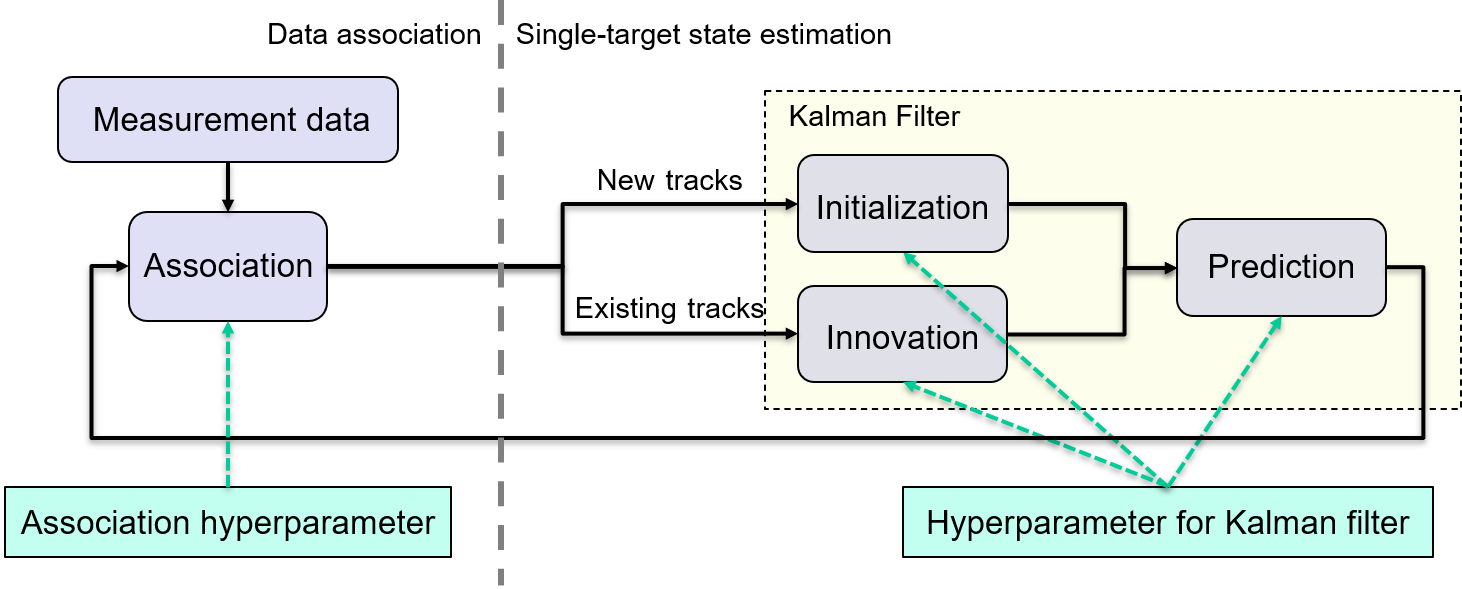
\includegraphics[width=0.9\textwidth]{figures/tracking system.png}
\caption{Structure of the multitarget tracking algorithm.}
\label{tracking system}
\end{figure}

% \subsection{Data Association}

In the tracking problem, we need to update the new state of each object with the measurement data. However, in the multitarget tracking problem the correspondence information between each measurement and object is usually not provided. Therefore, we need the data association algorithms to establish this correspondence. With the data association, each measurement is assigned to an object. Then the original multitarget tracking problem is transferred into many single-target tracking problems that are much easier to solve.

There are many types of data association algorithms. A basic idea is to assign the measurement to the object, whose predicted position is closest to the measurement. When the assignment process is done consecutively, this method is the local nearest neighbor (LNN). However, this method often leads to incorrect association decisions, as shown in Figure \ref{lnn} \cite{pfaff2019multitarget}.

\begin{figure}[htbp]
\centering
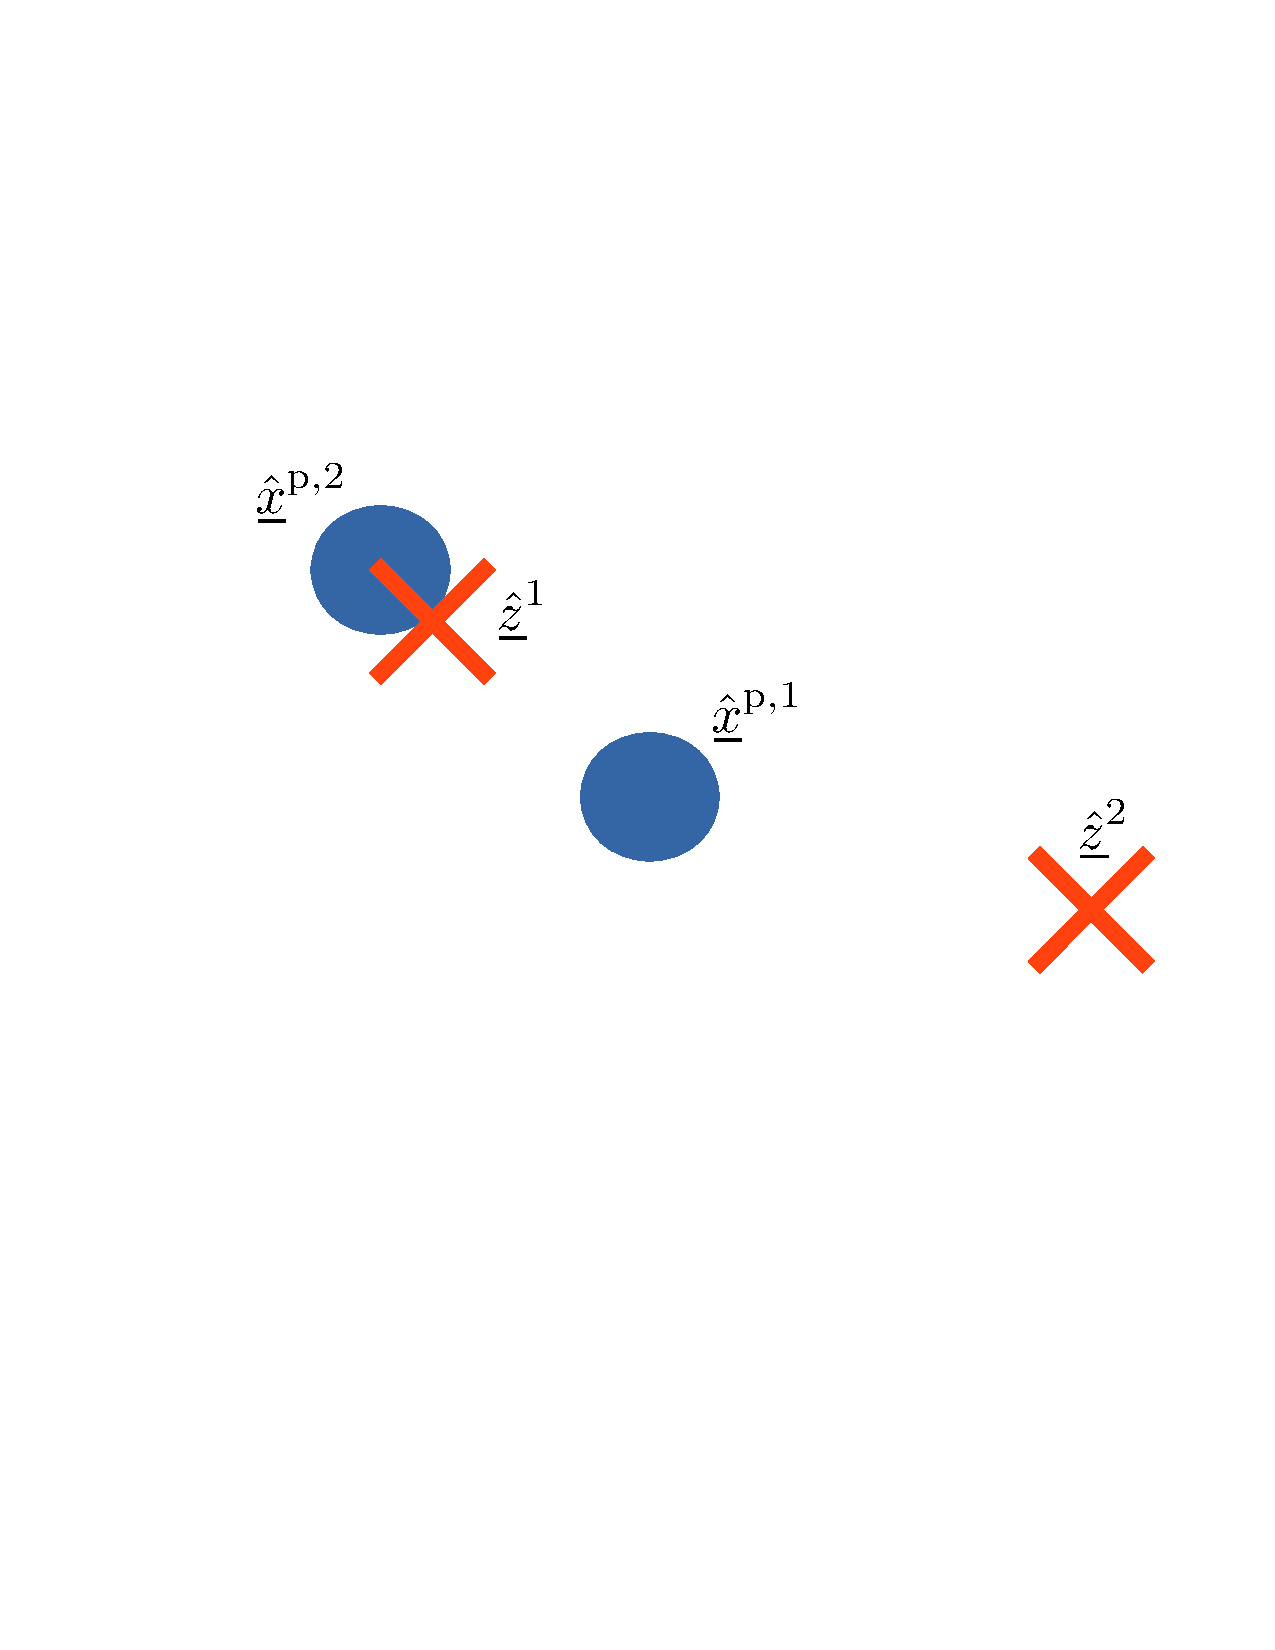
\includegraphics[width=0.5\textwidth]{figures/LNN.pdf}
\caption{Example in which the LNN may perform badly. If the $\hat{\underline{z}}^{2}$ is assigned before $\hat{\underline{z}}^{1}$, it will be assigned to $\hat{\underline{x}}^{\mathrm{p},2}$, which leads to an association error \cite{pfaff2019multitarget}.}
\label{lnn}
\end{figure}

The global nearest neighbor (GNN) optimizes the overall quality of the association decision by determining the association decision that minimizes the sum of the distances of all track–measurement pairs. 
% \textcolor{red}{I deleted the "squared Mahalanobis" here, because I think only mentioning the distance is enough for explaining the principle of GNN. The Mahalanobis is in detail explained in the next chapter.} 
The GNN has more complexity than the LNN, but it can significantly improve the accuracy of the association. Therefore, the GNN is chosen from the multitarget tracking algorithm. 
% The more detailed description of the implementation of the GNN and tracking algorithm is presented in \Sec{mt}. 

One extension of the GNN is the multi-hypotheses tracking, where the algorithm gives several hypotheses of the association in each step of the tracking process, and the update processes are also done with different hypotheses. The most possible hypothesis in the end will be chosen as the final association result \cite{blackman2004multiple}. However, multi-hypotheses tracking is not suitable for real-time tracking in the implementation used in this thesis because of the high computational costs \cite{pfaff2019multitarget}. 

Until now, we are introducing the hard association methods that were used in our implementation, where each measurement is assumed to belong to exactly one object and each state updation is based on only one measurements. However, there are also several other data association methods using the soft association, where one measurement can be used to update several tracks. There are soft association algorithms using the joint probabilistic data association \cite{fortmann1983sonar} or the Markov chain Monte Carlo based particle filter \cite{khan2005mcmc}. However, these algorithms usually have high computational requirements and are sometimes hard to integrate with other parts of the implemented multitarget tracking algorithm we are using. For these reasons, these algorithms are not considered in the multitarget tracking algorithm used in this thesis.

In some cases, the feature of the objects can also be used for the association. Algorithms using the object features have been widely used in many areas, such as tracking of humans in videos \cite{wu2006tracking}. Following this idea, integrating the object information into the association can be a possible extension of the tracking algorithm.

% \subsection{State Update and Estimation}

% \textcolor{red}{still necessary here?}
% In the last part, the multitarget tracking problem is transferred into many single-target tracking problems. Therefore, a Kalman filter with a selected motion model is used for solving these problems. The Kalman filter updates the state prediction for each track, which is used for the data association of the next timestep. 

% The algorithm for this part is more detailed explained in \Sec{st}. 

\FloatBarrier

\section{Optimization Algorithms}

% \textcolor{red}{Added a very short introduction of the objective functions}
Optimization is the minimization or maximization of an objective function subject to constraints on its variables \cite{nocedal2006numerical}. There are many algorithms proposed for optimization, which can be mainly divided into two classes. One is the gradient-based optimization that computes the gradient of the loss function of the hyperparameters and then optimizes the hyperparameters using gradient descent. However, many systems are too complicated to have the explicated solution for the gradient of the loss function, which limits the application of the gradient-based optimization only on some specific problems, such as hyperparameter optimization in support vector machines \cite{chapelle2002choosing} or logistic regression \cite{foo2008efficient}. 

The other optimization methods, such as grid search, random search, Bayesian optimization and evolutionary algorithms need no gradient information of the loss function. These methods treat the system for optimization as a black box. In grid search, the main algorithm computes the loss function with a tuple of hyperparameters from the predefined parameter space in each search and selects the best hyperparameter set minimizing the loss function. Bayesian optimization creates a surrogate model from the observed value of the loss function replacing the original loss function, and determine the optimized point based on the surrogate model. Evolutionary optimization makes numerous observations in each step and breeds the observation point for the next timestep from the observation with lower losses. These methods have different features and are used in different scenarios \cite{claesen2015hyperparameter}\cite{feurer2019hyperparameter}.

% A hyperparameter is a parameter of a learning algorithm that is set prior to training and remains constant during training.

\subsection{Objective Function}

The objective function evaluates the performance of a model or an algorithm on the given data. An objective function is either a loss function to be minimized, or a reward function that needs to be maximized. For example, the prediction error introduced in \Sec{loss function} is the loss function for our optimization.

Given a function $f(x,y)$, there can be two types of objective function with the difference of the optimizing object. The first type is to find the maximum or minimum of the function, as $\max f(x,y)$. The other type is to find the values of some variables within the constraints that minimize (or maximize) the objective function, for example, $\underset{x\in \mathbb R,\ y\in \mathbb R}{\arg \max }\ f(x,y)$. In general, we are more interested in the second type of object function.


There are different objective functions for different optimization problems. The functions always depend on the optimization objection. There are two important types of problems in machine learning: regression and classification. In regression, a model is trained for mapping the input variables to continuous output variables that fit the observations \cite{balasubramanian2014conformal}. Therefore, the mean squared error (MSE) $(\sum _{i=1}^{n}(y_{i}-{\hat {y_{i}}})^{2})/n$ and the mean absolute error (MAE) $(\sum_{i=1}^{n} \left | y_{i}-\hat{y_{i}} \right |)/n$, which show the distance between the observations and predictions, are the most common objective functions. In the expression, the $y_{i}$ and $\hat{y_{i}}$ means respectively the $i$th observed and predicted value, and the $n$ indicates the number of predictions. 

The classification problem needs to approximate a mapping function (f) from input variables to discrete output variables. Therefore, the MSE and MAE can be also used in the classification problem for evaluating the difference between the predicted and observed classes. There are also some common loss functions only for discrete classes, such as the cross-entropy loss $-\sum_x p(x)log\,q(x)$, where the $p$ and $q$ indicates observed and predicted probability distribution.






% \textcolor{red}{But most of optimization problem like $\arg \max \ f(x,y)$ is able to obtain the $\max f(x,y)$ at the same time?}

% \textcolor{red}{To some extent the optimization of hyperparameters is also a type of regression? Find hyperparameters to build a model to fit the measurements(input) and the last measurements of tracks(output). The loss function is MAE for prediction error of each track.}
% Although there are

% \textcolor{red}{Is it all right for these math expressions stay in text or it should in a separated display?} 

% \textcolor{red}{Should I give a more detailed description of the regression problems?} 



% \textcolor{red}{And should I give a more detailed description of the classification problems? The SVM has its own loss function.} 

\subsection{Grid Search}
\label{gs}

% \textcolor{red}{define the HP}

Grid search is the most traditional and intuitive way for the optimization of hyperparameters \cite{ataei2004using}. The procedure of grid search is shown in Figure \ref{grid search}. At first, a set of sample values are determined for each hyperparameter for optimization. Then the main algorithm of grid search runs with hyperparameters in the Cartesian product of these sets, which is the so-called grid points, and evaluates the performance with the value of the objective function \cite{bergstra2012random}. 

Since the grid search algorithm returns the value of the objective function of all grid points, it is possible to evaluate the effect of different hyperparameters on the objective function, as the blue area shown in Figure \ref{grid search}. The best hyperparameter set can also be chosen as the hyperparameter set that results in the minimum error.

\begin{figure}[htb]
\centering
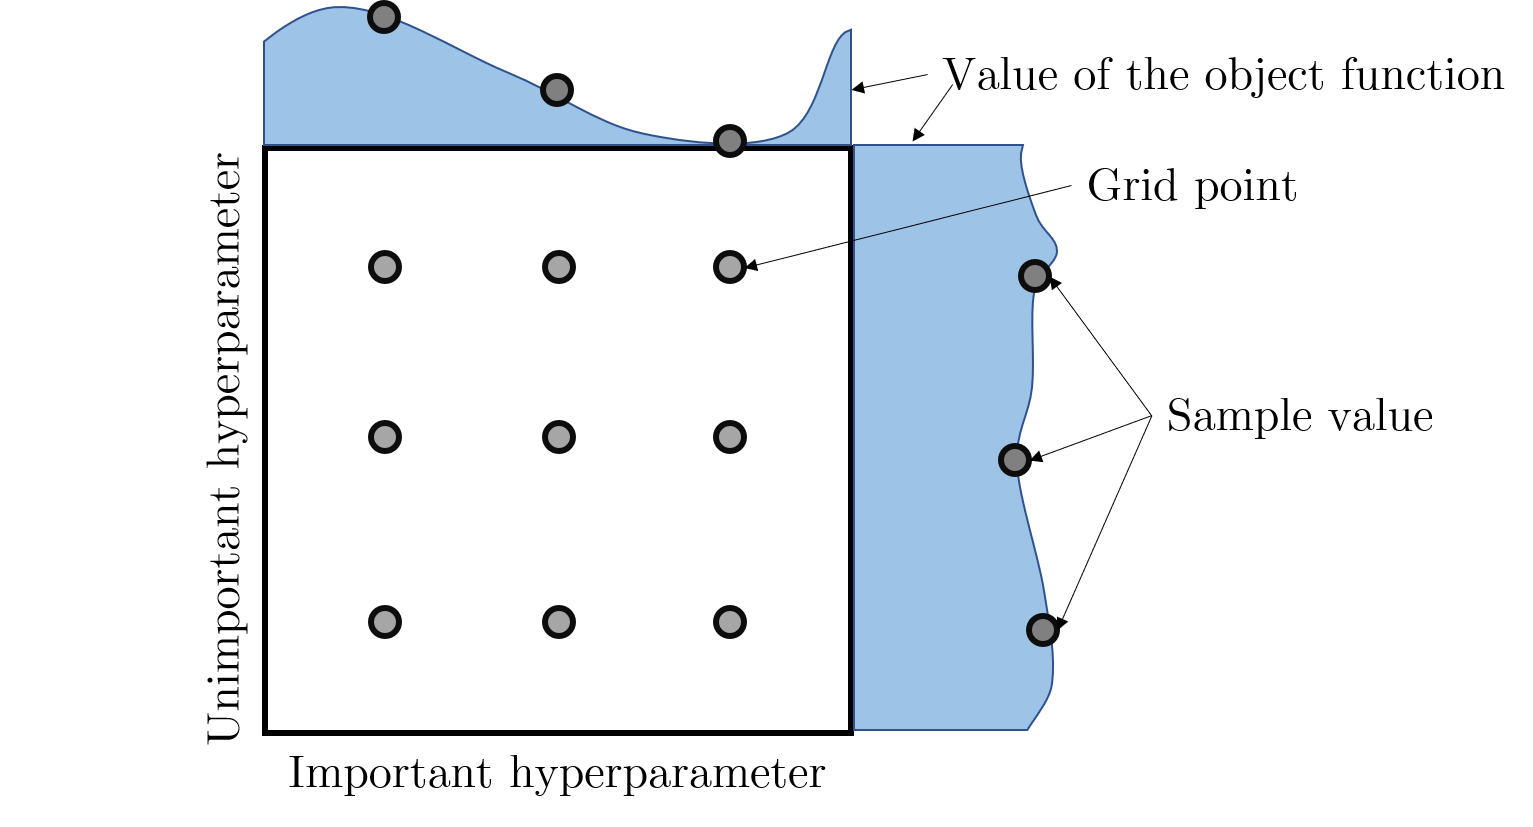
\includegraphics[width=0.8\textwidth]{figures/grid search.png}
\caption{Illustration of grid search, showing the sample points, grid points and different effects of the hyperparameters on the value of the objective function \cite{bergstra2012random}.}
\label{grid search}
\end{figure}

Grid search is easy to implement and understand, but not efficient. First, the grid points to check in grid search increases exponentially with the number of hyperparameters, thus grid search is not practical with too many hyperparameters. Second, the grid points need to be chosen manually before the optimization, which means choosing the appropriate sample values of the hyperparameter can be challenging work. Furthermore, the searches are limited in the grid points, so the final optimized point provides not necessarily the real optimal value of hyperparameters. At last, each search in grid search can be independent. It means that the selection of hyperparameters of each search can not use the information of the objective function from former searches, which is a waste of the computation power \cite{bergstra2012random}. For the reasons above, grid search is often combined with other optimization methods, which used for giving an initial impression of the effect of hyperparameters or reducing the dimension of hyperparameters for the next step of optimization \cite{ataei2004using}.

\subsection{Bayesian Optimization}
\label{bayopt intro}

% \textcolor{red}{todo: rewrite this part with less words and more equations}

Bayesian optimization is a state-of-the-art optimization framework for the global optimization of functions. Bayesian optimization only depends on the discrete observed values of the objective function, without using any gradient information of the objective function. This method is one of the most efficient approaches in terms of the number of function evaluations required. Therefore, this method suits especially the problems, where the objective function is unable to be expressed with a differentiable function or expensive to calculate \cite{brochu2010tutorial}.

\begin{figure}[htbp!]
\centering
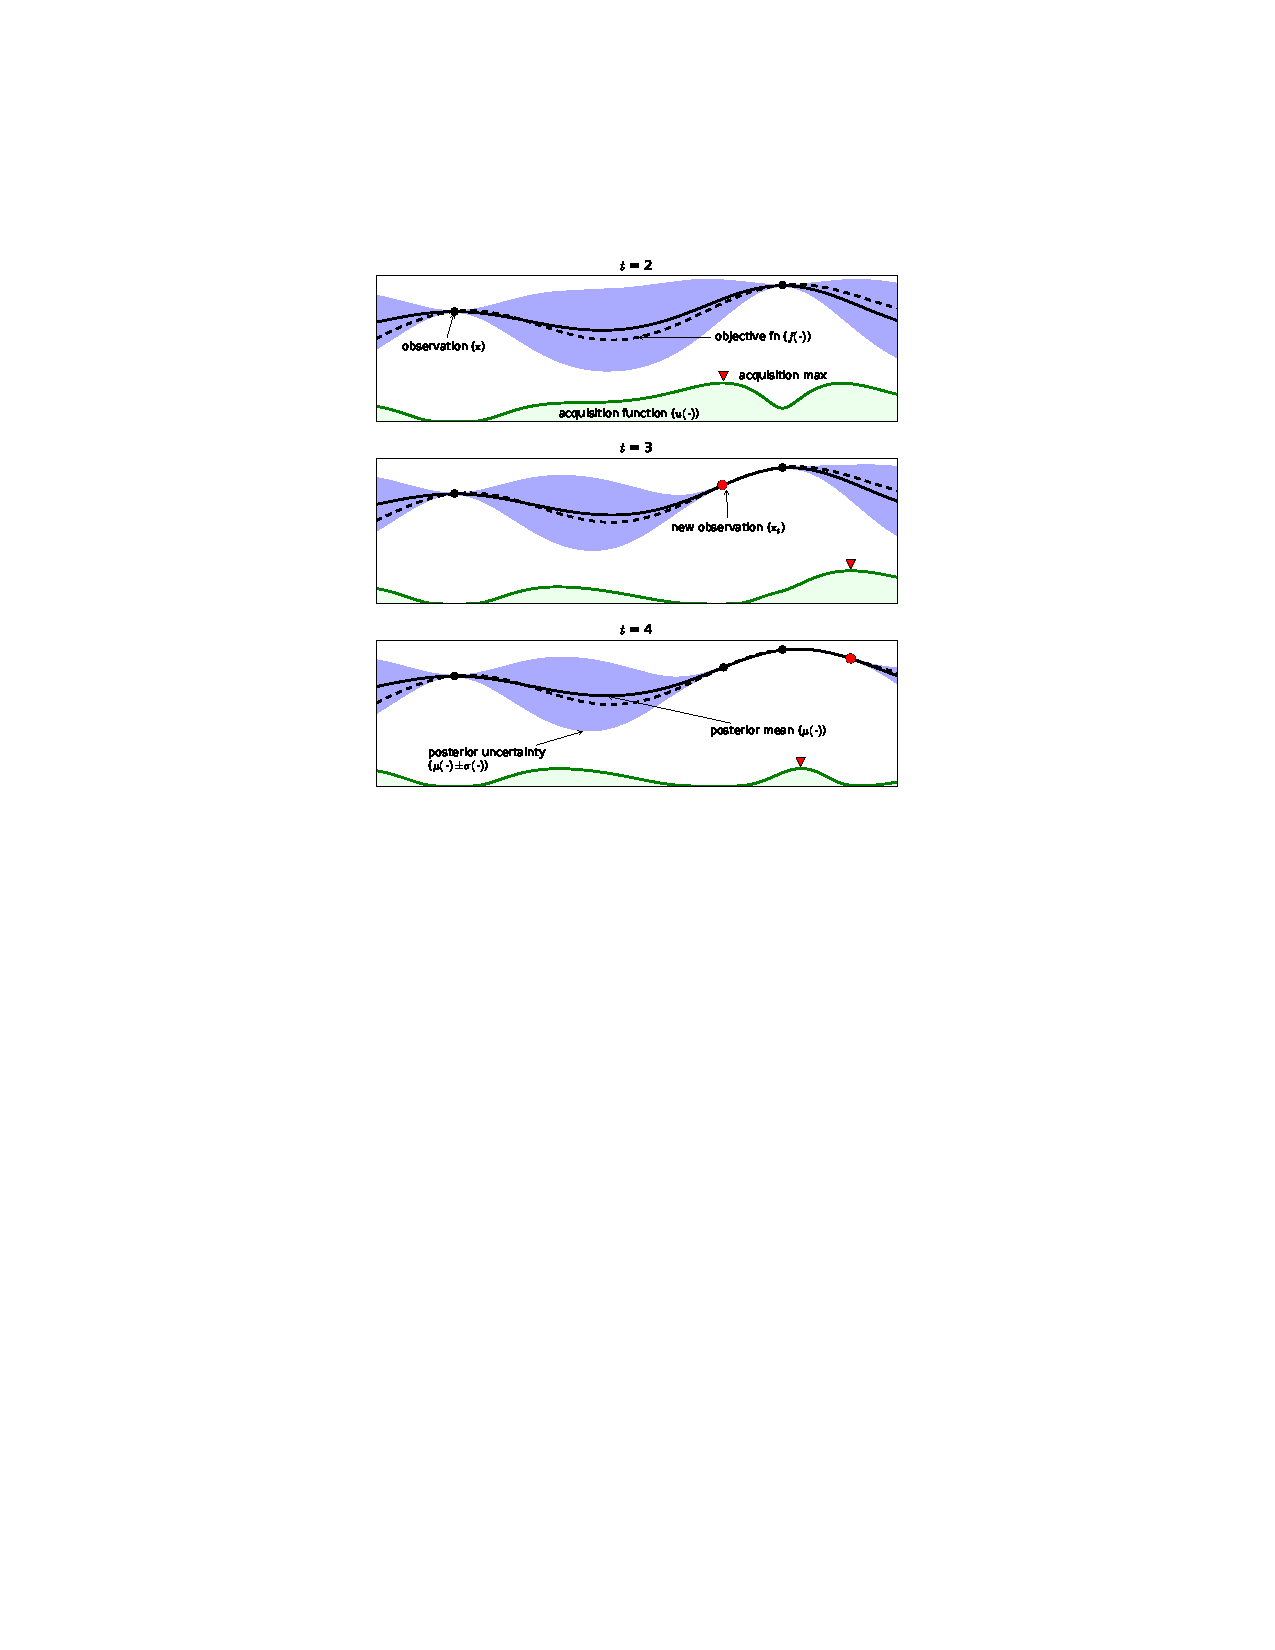
\includegraphics[width=0.8\textwidth]{figures/bay opt.pdf}
\caption{The figures demonstrate an example of Bayesian optimization. The posterior means function of the surrogate model is shown in the black solid line, and the original objective function is shown in the black dash line. After each iteration, the surrogate model is updated according to the observation result. The blue shade shows the variance of the model. The unsampled area has high uncertainty, and uncertainty at observed points is reduced to 0. The acquisition function is shown in the lower green shaded plots. When the estimated objective function or uncertainty is high, the acquisition is also high, which indicates a high possibility for the maximum of the objective function. The sample point for the next iteration is chosen from the maximum of the acquisition function, as the red triangle marks shown at $t=3$ and $t=4$ \cite{brochu2010tutorial}.}
\label{bayesian optimization}
\end{figure}


% \begin{algorithm}[!h]
% \caption{Bayesian optimization \cite{shahriari2015taking} \textcolor{red}{line number?need improve}}
% \label{Bayesian optimization algorithm}
% \begin{algorithmic}[1]
%     \FOR{$t=1,2,....$}
%         \State Select new $\mathbf{x}_{t+1}$ by optimizing acquisition function $\alpha$: \\ $\mathbf{x}_{t}=\mathop{\argmax}_{\mathbf{x}}{\alpha(\mathbf{x};\mathcal{D}_{1:t-1})}$\\
%         \State Make the observation: $y_{t}=f(\mathbf{x}_{t+1})+\varepsilon_{t}$ 
%         \Comment{Expensive step} \\
%         \State Augment data: $\mathcal{D}_{1:t}=\{\mathcal{D}_{1:t-1},(\mathbf{x}_{t},y_{t})\}$
%         \State update statistical model
%     \ENDFOR
% \end{algorithmic}
% \end{algorithm}


Bayesian optimization is an iterative algorithm that updates a probabilistic surrogate model $f(\mathbf{x})$ and an acquisition function $\alpha$ after every iteration. The surrogate model is an estimation of the objective function that is based on the value of observations of the objective function from each iteration. With this model, the algorithm can avoid estimating the original objective function, which is often too complicated. After enough iterations, the posterior mean function of the surrogate model will become similar to the objective function.

The Gaussian process (GP) prior is well-suited as the surrogate model. A GP is a random function represented with its mean function $m$ and covariance function $k$
\begin{equation}
    f(\mathbf{x}) \sim \mathcal{G} \mathcal{P}\left(m(\mathbf{x}), k\left(\mathbf{x}, \mathbf{x}^{\prime}\right)\right).
\end{equation}
This function returns the mean and variance of a normal distribution over the possible values of $f$ at $\mathbf{x}$ \cite{brochu2010tutorial}. One of the very common covariance functions is the squared exponential function
\begin{equation}
    k\left(\mathbf{x}_{i}, \mathbf{x}_{j}\right)=\exp \left(-\frac{1}{2}\left\|\mathbf{x}_{i}-\mathbf{x}_{j}\right\|^{2}\right).
\end{equation}
Given the first $t$ observation samples, we can use the Gaussian process to calculate the possible distribution of the observations using the Sherman-Morrison-Woodbury formula \cite{sherman1950adjustment}, namely
\begin{equation}
    P\left(f_{t+1} | \mathcal{D}_{1 : t}, \mathbf{x}_{t+1}\right)=\mathcal{N}\left(\mu_{t}\left(\mathbf{x}_{t+1}\right), \sigma_{t}^{2}\left(\mathbf{x}_{t+1}\right)\right),
\end{equation}
where
\begin{gather}
\mu_{t}\left(\mathbf{x}_{t+1}\right) =\mathbf{k}^{T} \mathbf{K}^{-1} \mathbf{f}_{1 : t} \\ 
\sigma_{t}^{2}\left(\mathbf{x}_{t+1}\right) =k\left(\mathbf{x}_{t+1}, \mathbf{x}_{t+1}\right)-\mathbf{k}^{T} \mathbf{K}^{-1} \mathbf{k}\\ \mathbf{K}=\left[\begin{array}{ccc}{k\left(\mathbf{x}_{1}, \mathbf{x}_{1}\right)} & {\dots} & {k\left(\mathbf{x}_{1}, \mathbf{x}_{t}\right)} \\ {\vdots} & {\ddots} & {\vdots} \\ {k\left(\mathbf{x}_{t}, \mathbf{x}_{1}\right)} & {\dots} & {k\left(\mathbf{x}_{t}, \mathbf{x}_{t}\right)}\end{array}\right].
\end{gather}

The acquisition function guides the selection of the sample point for the next iteration step, using the predicted distribution of the surrogate model. The acquisition function is designed for showing the potential maximum of the objective function, where the prediction or the uncertainty is high. There are many different criteria for the computation of the acquisition function. The probability of improvement acquisition function maximizes the probability of the value of objective function higher than the observed maximum objective value, as
\begin{equation}
    \mathrm{PI}(\mathbf{x}) =P\left(f(\mathbf{x}) \geq f\left(\mathbf{x}^{+}\right)+\xi\right),
\end{equation}
where $\mathbf{x}^{+}$ denotes the maximum value observed in former timesteps and $\xi$ indicates a trade-off parameter controlling the exploration and exploitation. When $\xi$ is high, the algorithm would have more tendency of exploration.

The expected improvement acquisition function maximizes the expected improvement with respect to $f(\mathbf{x}^{+})$. The expected improvement function is defined as
\begin{align} 
\centering
\mathrm{EI}(\mathbf{x}) &=\left\{\begin{array}{ll}{\left(\mu(\mathbf{x})-f\left(\mathbf{x}^{+}\right)-\xi\right) \Phi(Z)+\sigma(\mathbf{x}) \phi(Z)} & {\text { if } \sigma(\mathbf{x})>0} \\ 
{0} & {\text { if } \sigma(\mathbf{x})=0}\end{array}\right.\\, \end{align}
\begin{equation}
    Z =\frac{\mu(\mathbf{x})-f\left(\mathbf{x}^{+}\right)-\xi}{\sigma(\mathbf{x})} ,
\end{equation}
where $\phi(\cdot)$ and $\Phi(\cdot)$ denote respectively the PDF and CDF. $\xi$ is still a trade-off parameter for controlling the exploration and exploitation here.

The computation of the acquisition function needs balancing the trade-off of exploiting and exploring. This task can be accomplished by setting different values of the exploration ratio, as shown in Figure \ref{bayesian optimization2}. When the exploration ratio is low, or choosing to exploit, as choosing points where the surrogate mean is high, the optimized result can converge faster, but it also easier to stick into a local minimum. When choosing exploring, as choosing points where the surrogate variance is large, the algorithm is more possible to find the global minimum, but it can also take more iterations. Except for the trade-off parameter $\xi$ mentioned above, another method named \textit{Plus} using the exploration ratio $t_{\sigma}$ was introduced by Bull \cite{bull2011convergence}. Let $\sigma_{F}(\mathbf{x})$ be the standard deviation of the posterior objective function at $\mathbf{x}$ and $\sigma$ be the posterior standard deviation of the additive noise. When the $\sigma_{F}(\mathbf{x})<t_{\sigma}\sigma$, the algorithm declares that the algorithm is overexploiting at $\mathbf{x}$. Then the acquisition function modifies its kernel function a point $\mathbf{x}$ that is not overexploiting is generated.


\begin{figure}[htb]
\centering
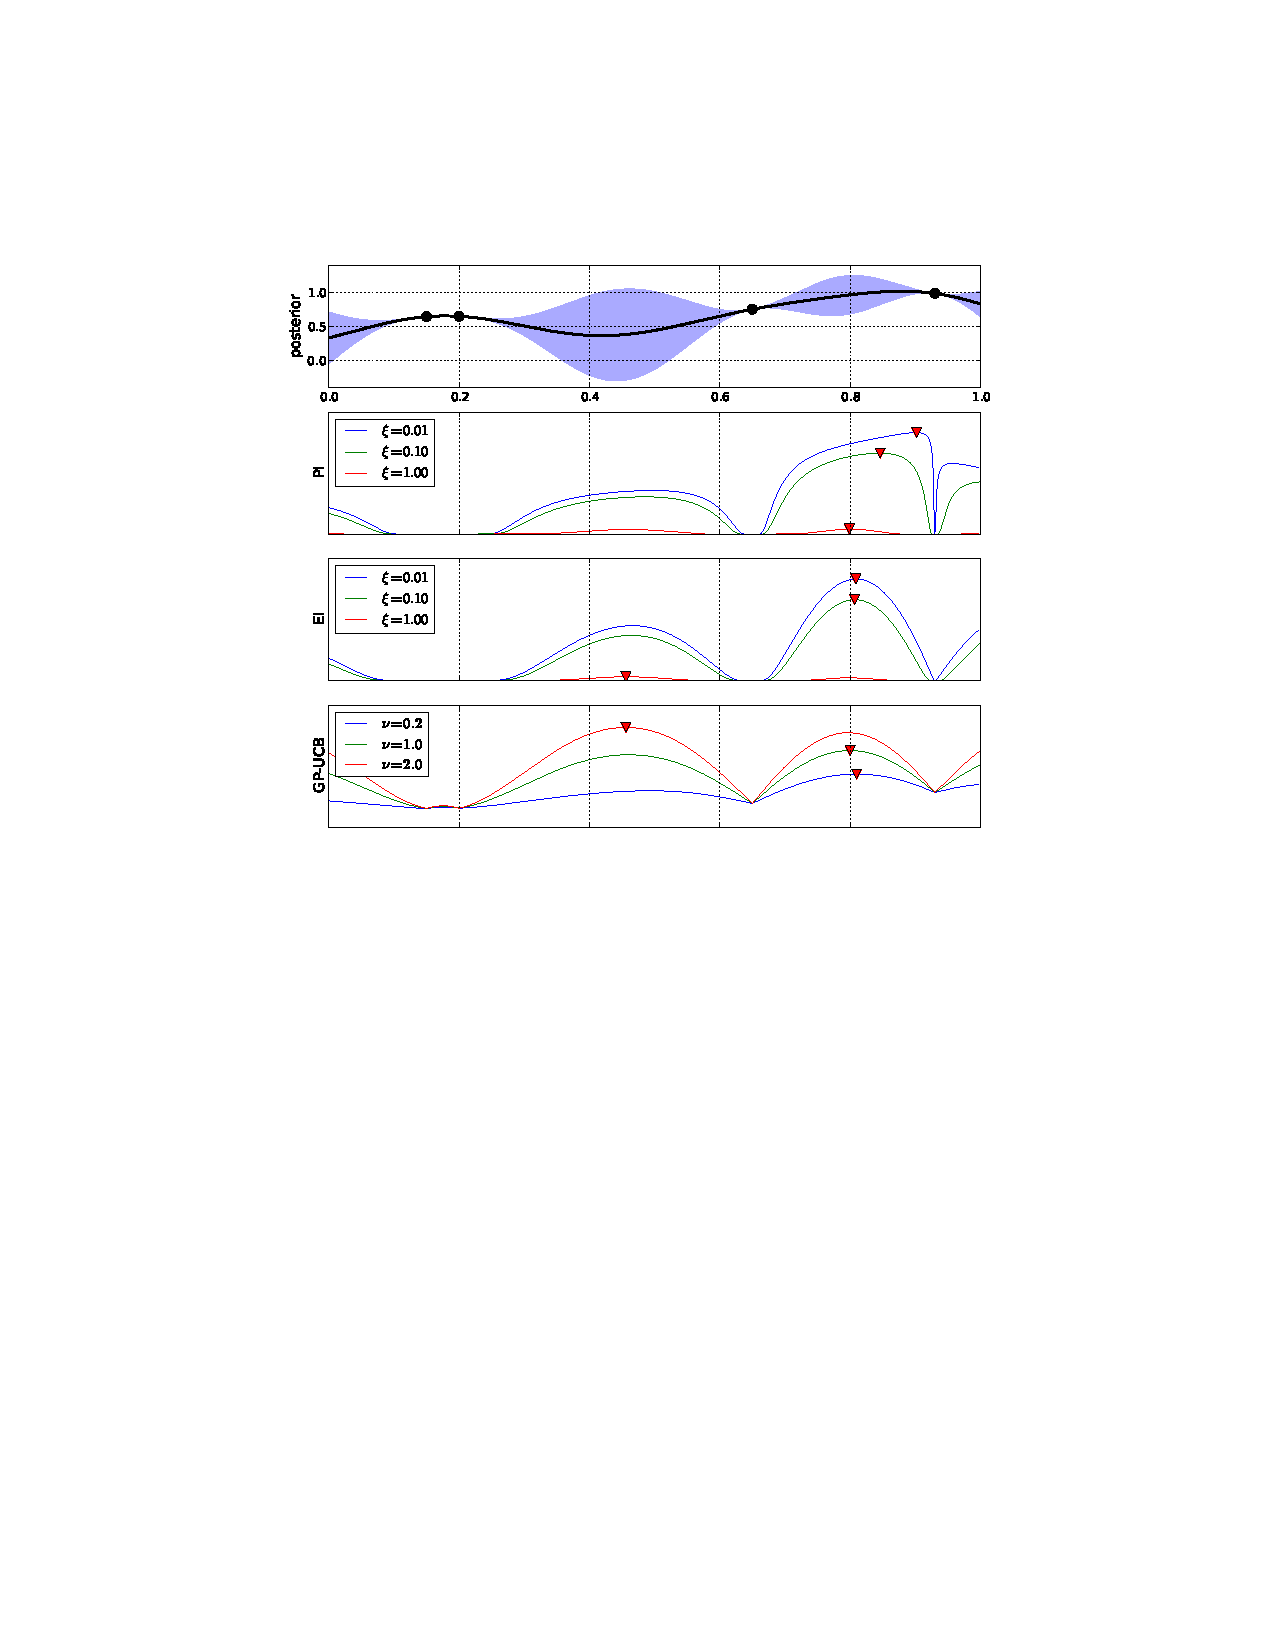
\includegraphics[width=0.8\textwidth]{figures/bayopt_acqui.pdf}
\caption{The figures demonstrate examples of acquisition functions in different settings. The black points indicate the observations. The red triangles indicate the maximum of the acquisition functions. The $\xi$ and $\nu$ are the hyperparameters that have a similar effect of the exploration ratio, where a higher value means choosing exploring more \cite{brochu2010tutorial}.}
\label{bayesian optimization2}
\end{figure}

The time for evaluating the objective function can also depend on the value of the hyperparameter. In \textit{Per Second}  method raised in \cite{snoek2012practical}, the Bayesian optimization algorithm maintains a model of the objective function evaluation time $\mu_{s}(\mathbf{x})$ besides the main surrogate model. The acquisition function with this method is calculated with 
\begin{equation}
    \mathrm{EI}_{ps}(\mathbf{x})=\frac{\mathrm{EI}(\mathbf{x})}{\mu_{s}(\mathbf{x})}.
\end{equation}



\FloatBarrier

\section{Classification Algorithms: Support Vector Machine}

Statistical classification is a supervised learning problem of training a model categorizing new, unlabeled data based upon its relevance to known, labeled data. From the results of the classifiers we can also obtain the decision boundary of the data, which can be used for the determination of the range of the hyperparameters in our implementation. There are a large number of classification methods, such as logistic regression, support vector machines, k-nearest neighbors and neural networks.

\subsection{Basics of the Support Vector Machines}

Support vector machines (SVM) are a set of supervised learning methods used for classification, regression and outliers detection \cite{suykens1999least}. The support vector machines are trained with training examples labeled with different categories. A trained SVM can show the classification boundary between categories and classify unknown examples into a category.

The basic idea of SVM is to find a hypersurface splitting different categories that maximize the distance from data points to the hypersurface. Classifiers with this hypersurface can minimize the risk of the classification \cite{vapnik1999overview}. In a typical binary classification problem, the training set is given as $N$ data points $\{x_{i},y_{i}\}^{N}_{i=1}$, where $x_{i} \in \mathbb{R}^n$ is the $i$th input pattern and $y_{i} \in \mathbb{R}$ is the $i$th output pattern. A linear support vector machine constructs a classifier of the form
\begin{equation}
f(x)=\mathrm{sign}( w^\top x +b).
\end{equation}

To ensure the robustness of the classification, the distance between data points and classification hypersurface should be higher than a margin. For simplicity, the margin is often set at 1, which can be presented as
\begin{equation}
y_{i}(w^\top x_{i}+b)\geqslant 1.
\end{equation}


In case the separation hypersurface is not existed, some of the data points are allowed to locate more close to the hypersurface or even locate at the other side of the plane. Therefore, a slack variable $\xi_{i}$ is introduced, and the constraints for the classifier can be represented as
\begin{equation}
y_{i}(w^\top x_{i}+b)\geqslant 1 - \xi_{i},
\end{equation}
\begin{equation}
\xi_{i}\geqslant 0.
\end{equation}

The distance between the data points and the hypersurface can be represented as $\frac{y_{i}(w^\top x_{i}+b)}{\left \| w \right \|}$. Moreover, the summation of the slack variables $\xi_{i}$ should be minimized, the objective function can be represented according to \cite{suykens1999least} as 

\begin{equation}
L(w, \xi_{i})=\frac{1}{2}\left \| w^{2} \right \|+c\sum_{i=1}^{N} \xi_{i}.
\label{regularization svm}
\end{equation}
Here $c$ is a parameter determines the trade-off between increasing the margin size and ensuring that the ${\vec {x}}_{i}$ lie on the correct side of the margin.

\subsection{Nonlinear Kernels}

In order to deal with the nonlinear classification problems, nonlinear transition functions are introduced to replace the dot product kernel function in the linear SVM. The transition function maps the input space into a higher dimensional space. The new classifier with a nonlinear transition function $\phi(\cdot )$ can be represented as

\begin{equation}
f(x)=\mathrm{sign}( w^\top \phi(x) +b).
\end{equation}

The kernel function can represent the transition function implicitly. Then the SVM is able to be trained in that feature space and have the nonlinearity without explicit computation of the transition function. A general kernel $k$ has the relationship with the transition function as follows

\begin{equation}
k(\mathbf{x}, \mathbf{x'}) =\frac{\| \phi(\mathbf{x}) \|^2+\| \phi(\mathbf{x'}) \|^2-d(\phi(\mathbf{x'}),\phi(\mathbf{x'}))^2}{2}.
\end{equation}

One of the most widely used kernel function is the Gaussian radial basis function (RBF) kernel \cite{vert2004primer}

\begin{equation}
k_{g}(\mathbf{x}, \mathbf{x'}) = \exp\left(-\frac{\|\mathbf{x} - \mathbf{x'}\|^2}{2\sigma^2}\right).
\end{equation}
The Gaussian kernel will be used in the following part of the thesis.


\section{Overfitting and Remedy}

% \textcolor{red}{new section}

In machine learning problems including regression and classification, overfitting means the trained model fits so exactly to the training dataset, that fails to predict future observations in more general cases. This problem often happens when the prediction model in training is much more complex than the model of the dataset, or the training dataset is not large enough to show the general characteristic of the whole dataset that we are interested in. In this case, the model learns not only the information but also the noise in the training data, and a high accuracy on the training data does not imply a high accuracy on the whole data. To overcome overfitting, many methods have been introduced into the machine learning area, such as regularization, cross-validation, early stopping, or dropout.

\begin{figure}[htb]
\centering
\begin{subfigure}[t]{0.4\textwidth}
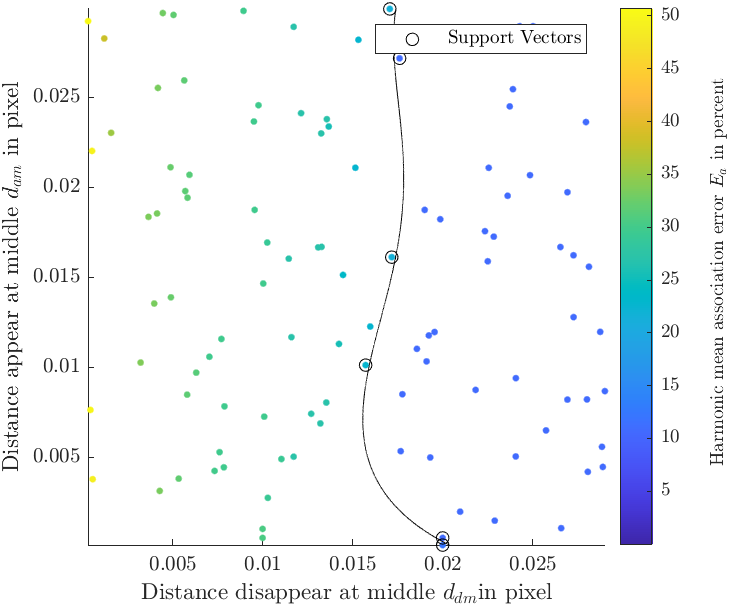
\includegraphics[width=\textwidth]{figures/Asso/overfitting2.png}
\caption{An SVM classification without overfitting. The kernel size is set as 0.5.}
\end{subfigure}
% \hfill
\quad
\begin{subfigure}[t]{0.4\textwidth}
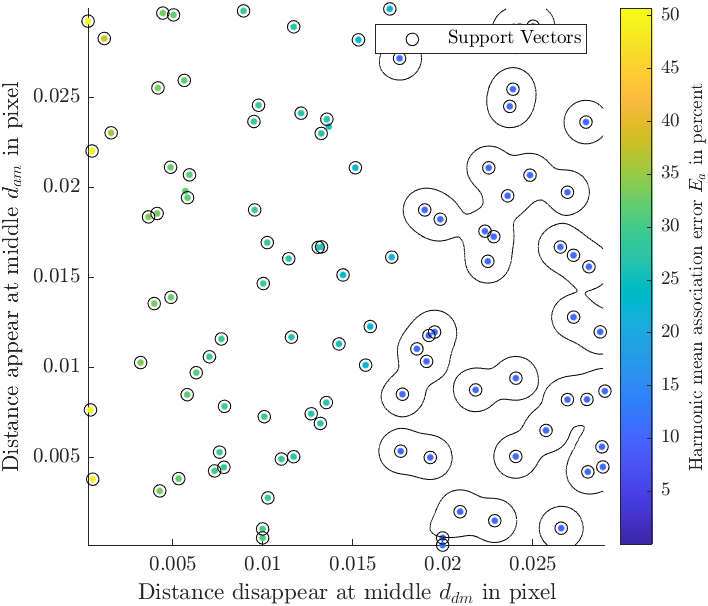
\includegraphics[width=\textwidth]{figures/Asso/overfitting1.png}
\caption{An SVM classification with overfitting. The kernel size is set as 0.01.}
\label{overfitting example}
\end{subfigure}
\caption{Overfitting in the SVM. In Figure (b) the robust area is limited only around the training points, which leaves all the other area as unrobust area.}
% \label{overfitting}
\end{figure}

\subsection{Regularization}

Many loss functions only evaluate how the prediction model from training fits the data, but complexity of the prediction model is ignored. Therefore, the prediction model can be severely affected by the noise of each single training data point and have many unnecessary complexity, such as a highly curved decision boundary in classification problem or a polynomial regression model with high degree terms. Regularization brings the model information into the loss function so that the model can keep as simple as possible and eliminate the misleading effect from the high-frequency noise in the training data. In the typical regularization method, a regularization term is added into the loss function to apply a penalty on the complexity of the prediction model $f$ , as
\begin{equation}
L(f,y)=\sum_{i=1}^{n}V(f(x_{i}),y_{i})+\lambda R(f),
\end{equation}
where $V$ is the original loss function and $R$ is a function that presents the complexity of $f$ \cite{poggio1985computational}. 

The regularization method was first raised in the linear regression problem. A linear model $f(\underline{x})=\underline{\omega}^\top \underline{x}$ is characterized with the vector $\underline{\omega}$. In order to minimize the complexity of the model, the $L_{1}$ and $L_{2}$ regularization, which take the 1-norm and 2-norm of $\underline{\omega}$ as the regularization term, are used \cite{ng2004feature}. The $L_{1}$ and $L_{2}$ regularization is expressed with following equations
\begin{equation}
L_{1}(f,y)=\sum_{i=1}^{n}V(f(x_{i}),y_{i})+\lambda \sum_{j=1}^{m} \left| \omega_{j}\right|
\end{equation}
\begin{equation}
L_{2}(f,y)=\sum_{i=1}^{n}V(f(x_{i}),y_{i})+\lambda \sum_{j=1}^{m}\omega_{j}^2
\end{equation}

In SVM, the first term $\frac{1}{2}\left \| w^{2} \right \|$ in the loss function in Equation \Eq{regularization svm} can serve as a regularization term. Therefore, no additional regularization terms are needed. The parameter $c$ can control the importance of the regularization term, where a higher $c$ means the classifier is more regularized \cite{evgeniou2000regularization}. 

In SVMs with Gaussian kernel, selecting the suitable kernel size $\sigma$ can also reduce the chance of overfitting. A higher kernel size means the range of influence of each support vectors is larger, and the number of support vectors is less. As a result, choosing a higher kernel size can help to avoid overfitting. Figure \ref{overfitting rbf} shows the effect of the regularization parameters $c$ and $\sigma$ on the shape of the classification boundary.

\begin{figure}[htb]
\centering
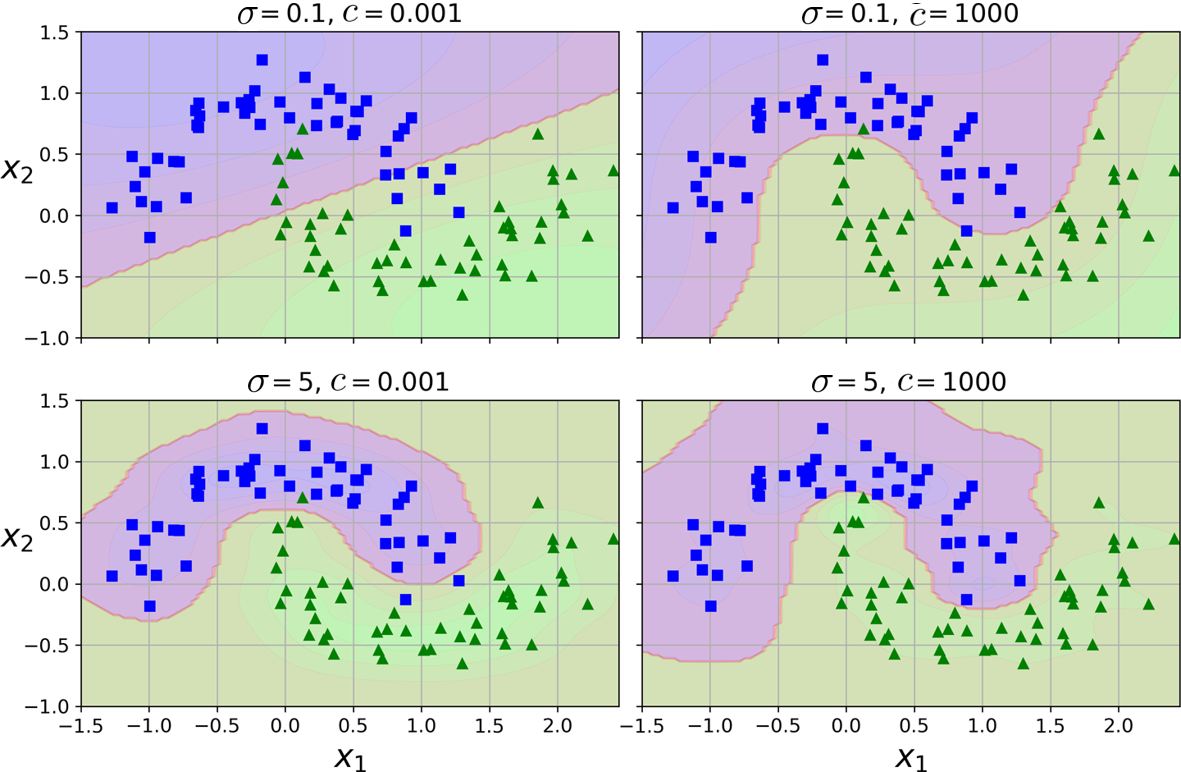
\includegraphics[width=0.8\textwidth]{figures/mls2_0509.png}
\caption{SVM classifiers with an RBF kernel using different regularization parameters \cite{geron2019hands}.}
\label{overfitting rbf}
\end{figure}

\subsection{Cross-Validation}

% \textcolor{red}{I think I mentioned the train-test split in the first paragraph. Is it too short or not clear?}

In order to examine how the trained model fits in the whole dataset, an easy method is the cross-validation. The whole dataset is separated into two sub-datasets: training dataset and test dataset. The prediction model is first trained with the training dataset, and then test the accuracy of the trained model with the test dataset. If the accuracy with the test dataset is also acceptable, the prediction model can be recognized as not overfitting.

However, the amount of data is usually limited. Therefore, it is a waste to use a part of data only for testing and leave the information contained in these data unused in training. The selection of test datasets can also have a great influence on model performance \cite{james2013introduction}. To reduce these effects, the cross-validation is preformed multiple rounds with different divisions, and the validation results from all rounds are combined for estimation of the general model performance.

K-fold cross-validation randomly splits the whole dataset into $k$ groups, or folds, of approximately equal size. In each training, a group is left out as the validation dataset, and the other $k-1$ groups are used as the training data. After doing $k$ times of training, we get $k$ model trained with different data. The final trained model takes the best fit model or the average of all models. With the $k$ times of training, all the information in the datasets can be learned by the prediction model, and the influence of the selection of the test dataset is minimized.

The most widely used $k$ value is 10, 5 and 1. When $k=1$, the method is also called leave-one-out cross-validation. Increasing $k$ increases the accuracy of training, but also increases the computational demand. There are also literatures reporting that the performance with $k=10$ is better than the leave-one-out cross-validation \cite{james2013introduction}.









    \chapter{State of the Art}

In the previous chapter, we introduced the basic idea of the tracking algorithm and the optimization methods. In this chapter, we first present more detailed knowledge of the implementation of the multitarget algorithm. In the first two sections, the basics of the traditional belt sorting system as well as the improvement in the \textit{TableSort}-System and the \textit{TrackSort} algorithm are presented. In Section 3.3, the implementation of the multitarget tracking algorithm is in detail explained, including the motion models used for tracking and the methods for data association and track management. Along these details, all the hyperparameters for optimizations in following chapters are listed.


\section{Overview of the Belt Sorting System}

Optical belt sorting is a versatile, state-of-the-art technology, which sorts bulk materials according to optical features. It usually comprises four parts: the feed system, the optical system, the data processing system, and the separation system, as illustrated in Figure \ref{belt sort system} \cite{edwards2004detecting}. The feed system usually consists of a material feeder and a conveyor belt or a slide, on which the materials flow through until being separated. This part can be also omitted, where the particles are in free fall before separation. The optical system contains cameras or sensors, which collect the location information of the material on the conveyor belt. The data processing system identifies the material and gives the prediction of the movement of the materials. Finally, the separation system separates the materials into different collectors.

\begin{figure}[htbp]
\centering
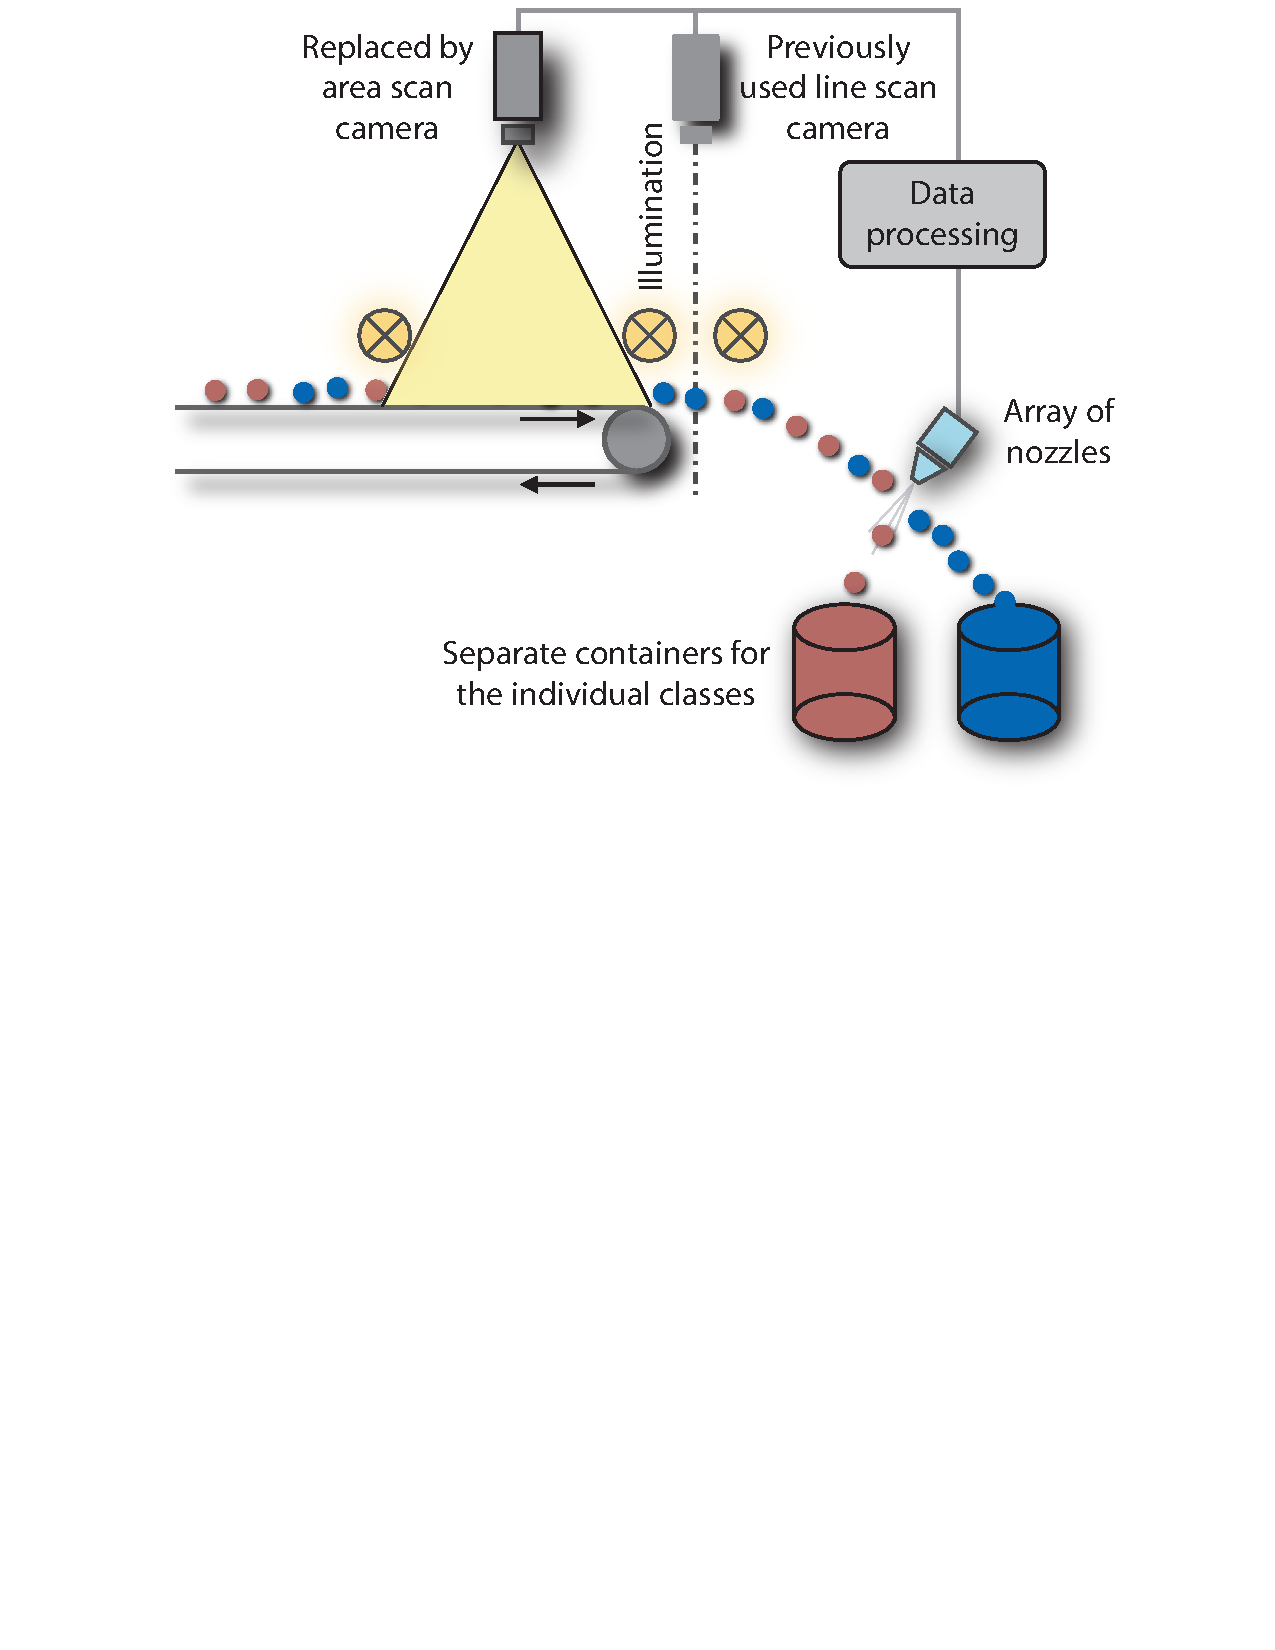
\includegraphics[width=0.6\textwidth]{figures/sort system.pdf}
\caption{Structure of a optical belt sorting system. In the recent research, the system with area scan camera has replaced the conventional system with line scan camera \cite{pfaff2017improving}.}
\label{belt sort system}
\end{figure}

The data processing system can be further divided into the image processing system, the tracking system and the prediction system. The image processing system transfers the image data from the camera into the particle centroid location and particle identity information. The tracking system tracks the movement of the particles in the tracking area and outputs the motion estimation of the particles. This part is also the main focus of this thesis. The prediction system predicts the time and location of the particles at the separator based on the information from the tracking system and certain motion models.
% \textcolor{red}{Add the traditional sorter here. The predictive sorting is moved to the next section.} 
Traditional optical belt sorters contain usually only line scan cameras or sensors, which observe the particles only once before the separator. As a result, traditional sorters can only gain a position measurement for each particle and can hardly do tracking on the particles. In the prediction system, because of the lack of the tracking information, the traditional optical belt sorters use the motion model that assumes the particles flying straightly in the transport direction without any motion orthogonal to the transport direction at a constant velocity, and the valve separator is activated after a fixed delay from detection of the particles. However, the particles do not always move straightly along the transport direction and may have a acceleration in flight. The motion model is not adequate for predicting such motion of the particles, which leads to a negative effect on tracking accuracy. 

\section{Introduction of \textit{TableSort} and \textit{TrackSort}}

The \textit{TableSort} system is a portable and flexible sorting platform, as shown in Figure \ref{fig:tablesortsystem}. One of the vital extensions of this system is to improve the separation results by utilization of the area scan camera and the predictive tracking method. The \textit{TableSort} system with the area scan camera can take several measurements for each particle in the tracking area and estimate the motion state of the particles. After the particles leave the tracking area, the predictive tracking algorithm can generate the predictions for the separation on the basis of the estimation from the tracking system and the motion model for the prediction part. This feature enables more accurate motion models in tracking and prediction.

\begin{figure}[htbp]
    \centering
	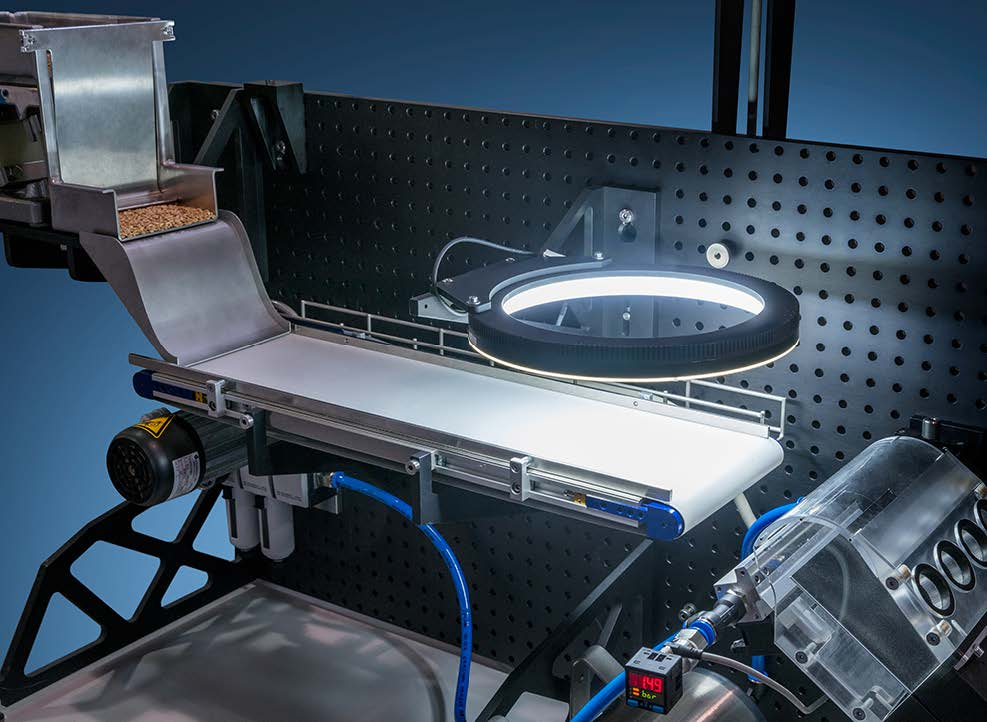
\includegraphics[width=0.8\textwidth]{figures/AT20-TrackSortMotionModels.jpg}
	\caption{Photo of \textit{TableSort} bulk material sorting system \cite{pfaff2020predictive}.}
	\label{fig:tablesortsystem}
\end{figure}

\section{Implementation of the \textit{TrackSort} Algorithm}

The \textit{TrackSort} algorithm developed by ISAS is used in the \textit{TableSort} system to estimate and predict the movement of each particle \cite{pfaff2015tracksort}. The process is divided into two phases. In the tracking phase, the position measurements on the belt are associated to each particle. With this position information, the motion of each particle is estimated by a recursive Kalman filter on the base of the motion model. This phase is the main focus of this thesis and will be further explained in the next section. After the particle has left the observation area of the camera, the algorithm enters into the prediction phase. The movement of the particles in this phase is predicted with the information from the tracking phase and the motion model, in order to determine an exact position and a time of separation. The motion models used in this phase are exhaustively introduced in \cite{pfaff2019multitarget}.

\subsection{Motion Models for Tracking}\label{Motion Models}

To balance the complexity and accuracy of the motion model, several assumptions are applied to different motion models. In belt sorting, we can assume that the material particles accelerate after touching the conveyor belt and then stay the same velocity with the belt. In this thesis, the constant velocity model (CV) and the constant velocity with angle model (CVA) are mainly used. Since the measurements are given in frame, only the discrete-time models are chosen.

\subsubsection{Constant Velocity Model}
% \textcolor{red}{Added the 2-D CV model.}

The constant velocity model is a widely used simple motion model for tracking particles that have entered a relatively stationary state with the belt. The 2-D CV model is used for the implementation of the tracking system. The noise terms in the motion model will be the hyperparameters for the sensitivity analysis and optimization.

In the 2-D constant velocity model, the state vector contains the position and velocity of the tracked objects along and vertical to the transport directions
\begin{equation}
    \underline{x}_{t}=
    \begin{bmatrix}
        \mathsf{x}_{t}\\ 
        \dot{\mathsf{x}}_{t}\\ 
        \mathsf{y}_{t}\\ 
        \dot{\mathsf{y}}_{t}
    \end{bmatrix}.
\end{equation}
Because the motion of the particles on different directions are considered as uncorrelated form each other, the system matrix for the constant velocity model is given as a block diagonal matrix with two system matrices from the 1-D CV model, as
\begin{equation}
    \mathbf{F}=\begin{bmatrix}
     1 & T & 0 & 0 \\ 
     0 & 1 & 0 & 0 \\ 
     0 & 0 & 1 & T \\ 
     0 & 0 & 0 & 1 
    \end{bmatrix}.
\end{equation}
In the implementation, the $T$ is always set as one, representing the time interval between each frame. Therefore, the time unit in this thesis will be frame.
The system noise covariance is also uncorrelated on different directions. Thus the matrix is given by
\begin{equation}
    \mathbf{C}^{\underline{\boldsymbol{w}}}=S^{\boldsymbol{w}}
    \begin{bmatrix}
     T^3/3 & T^2/2 & 0 & 0 \\ 
     T^2/2 & T     & 0 & 0 \\ 
     0 & 0 & T^3/3 & T^2/2 \\ 
     0 & 0 & T^2/2 & T 
    \end{bmatrix}.
\end{equation}
Only the position coordinates are directly observed in the measurement process. Therefore, the measurement matrix is
\begin{equation}
    \mathbf{H}=\begin{bmatrix}
     1 & 0 & 0 & 0 \\ 
     0 & 0 & 1 & 0 
    \end{bmatrix} .
\end{equation}
The measurement position covariance is a $2\times 2$ matrix. Because the measurement noise is generally uncorrelated on different directions and assumed to be same on different directions, it is given as the measurement variance multiplying an identical matrix, as
\begin{equation}
    \mathbf{C}^{\underline{\boldsymbol{v}}}= S^{\boldsymbol{v}}
    \begin{bmatrix}
     1 & 0 \\ 
     0 & 1
    \end{bmatrix} .
\end{equation}
Besides the parameters mentioned above, the initial parameters are also needed, as the initial position variance $S_{\mathrm{pos}}^{\mathrm{ini}}$, the initial velocity variance $S_{\mathrm{vel}}^{\mathrm{ini}}$ and the initial velocity guess $[\dot{\mathsf{x}}_{0}, \dot{\mathsf{y}}_{0}]$. In the implementation of  the \textit{TrackSort} algorithm, the initial variance is also assumed to be the same.  Therefore the initial estimated error covariance $\mathbf{C}_{0}^{\mathrm{e}}$ is given as
\begin{equation}
    \mathbf{C}^{\mathrm{e}}_{0}=
    \begin{bmatrix}
     S_{\mathrm{pos}}^{\mathrm{ini}} & 0 & 0 & 0 \\ 
     0 & S_{\mathrm{vel}}^{\mathrm{ini}} & 0 & 0 \\ 
     0 & 0 & S_{\mathrm{pos}}^{\mathrm{ini}} & 0 \\ 
     0 & 0 & 0 & S_{\mathrm{vel}}^{\mathrm{ini}}
    \end{bmatrix} .
\end{equation}
It is important to address that the initial velocity guess given from users is not always accurate. Therefore, when we have enough measurements, we use the average velocity calculated from measurements as the initial velocity guess for the initialization of new tracks instead. Because the initial velocity guess from measurements should be more close to the real initial velocity of the objects, the initial velocity variance should be lower. Therefore, the refined initial velocity variance $S_{\mathrm{vel}}^{\mathrm{ini, r}}$ is used after getting enough measurement data, which is different from the initial velocity variance $S_{\mathrm{vel}}^{\mathrm{ini}}$ used at the start of tracking. The hyperparameters in the CV model are listed in Table \ref{list hp cv}.
\begin{table}[htbp] 
    \centering
    \caption{List of hyperparameters for the CV model.} 
    \begin{tabular}{cc} 
    \toprule 
    Hyperparameters&Notation\\ 
    \midrule 
    Initial velocity guess              &$\underline{v}_{0}$\\
    Initial position variance           &$S_{\mathrm{pos}}^{\mathrm{ini}}$\\
    Initial velocity variance           &$S_{\mathrm{vel}}^{\mathrm{ini}}$\\
    Refined initial velocity variance   &$S_{\mathrm{vel}}^{\mathrm{ini, r}}$\\
    Measurement variance                &$S^{\boldsymbol{v}}$\\
    System noise variance               &$S^{\boldsymbol{w}}$\\ 
    \bottomrule 
    \end{tabular} 
    \label{list hp cv}
\end{table}

% Measurement noise density 

\subsubsection{Constant Velocity with Angle Model}

The constant velocity with angle model is similar to the constant velocity model, where the velocity of tracked objects are also considered as constant. However, the velocity of the tracked objects in the state vector of the CVA model is given with the magnitude of the velocity and the angle between the velocity and the transport direction. As a result, the state vector of this model contains the x- and y-coordinate of the object as well as the magnitude and the direction of the object velocity, as shown in Figure \ref{CVA}
\begin{equation}
    \underline{x}_{t}=
    \begin{bmatrix}
        \mathsf{x}_{t}\\ 
        \mathsf{y}_{t}\\ 
        \mathsf{v}_{t}\\ 
        \theta_{t}
    \end{bmatrix}.
\end{equation}
\begin{figure}[htbp]
	\centering
	\begin{subfigure}[t]{0.49\textwidth}
		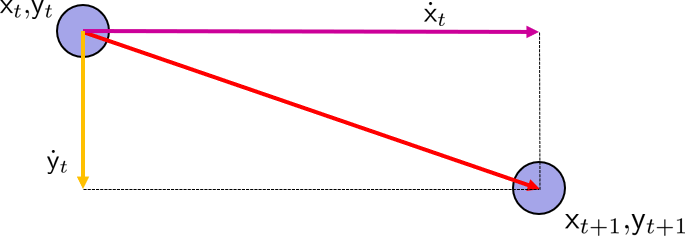
\includegraphics[width=\textwidth]{figures/CVmodel.png}
		\caption{CV model}
	\end{subfigure}
% 	\vskip\baselineskip
	\begin{subfigure}[t]{0.49\textwidth}
		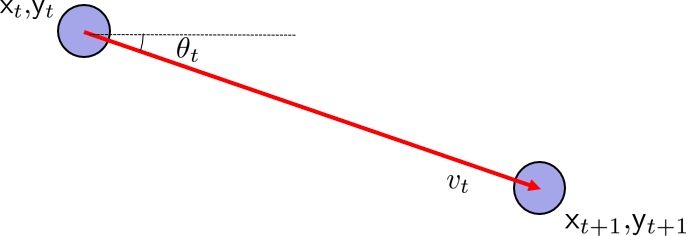
\includegraphics[width=\textwidth]{figures/CVAmodel.png}
		\caption{CVA model}
		\label{CVA}
	\end{subfigure}
	\caption{The illustration of the two motion models in this thesis.}
	\label{motion model}
\end{figure}
The relationship between state variables in the constant velocity model is not linear. Therefore, the predict and update processes of different state variables are done in three separated Kalman filter, and the variances for different state variables are also given separately. 

In the prediction step, the state transition function of the x- and y-coordinate of the object is given as
\begin{equation}
    \begin{bmatrix}
    \mathsf{x}_{t}^{\mathrm{p}}\\
    \mathsf{y}_{t}^{\mathrm{p}}\\
    \end{bmatrix}
    =
    \begin{bmatrix}
    \mathsf{x}_{t-1}^{\mathrm{e}}\\
    \mathsf{y}_{t-1}^{\mathrm{e}}\\
    \end{bmatrix}
    +
    \begin{bmatrix}
    \mathsf{v}_{t-1}^{\mathrm{e}}\cos\theta_{t}^{\mathrm{e}}\\
    \mathsf{v}_{t-1}^{\mathrm{e}}\sin\theta_{t}^{\mathrm{e}}\\
    \end{bmatrix}.
\end{equation}
The magnitude of the velocity and the angle between the velocity and the transport direction stay unchanged in the prediction step. The covariance for the position as well as the variance for the velocity magnitude and angle all follow the equation
\begin{equation}
    S_{t}^{\mathrm{p}}=S_{t-1}^{\mathrm{e}}+S^{\boldsymbol{w}}.
\end{equation}
% \begin{gather}
%     \mathbf{F}_{\mathsf{x},\mathsf{x}}=\begin{bmatrix}
%      1 & 0 & T\cos\theta & 0 \\ 
%      0 & 1 & T\sin\theta & 0 \\ 
%      0 & 0 & 1 & 0 \\ 
%      0 & 0 & 0 & 1 
%     \end{bmatrix} ,\\
%     \mathbf{C}^{\underline{\boldsymbol{w}}}=
%     \begin{bmatrix}
%      S_{\mathrm{pos}}^{\underline{\boldsymbol{w}}} & 0 & 0 & 0 \\ 
%      0 & S_{\mathrm{pos}}^{\underline{\boldsymbol{w}}} & 0 & 0 \\ 
%      0 & 0 & S_{\mathrm{vel}}^{\underline{\boldsymbol{w}}} & 0 \\ 
%      0 & 0 & 0 & S_{\mathrm{ang}}^{\underline{\boldsymbol{w}}}
%     \end{bmatrix} .
% \end{gather}
In the constant velocity with angle model, the position can be directly extracted from each frame of the measurement. The measurement value of the velocity magnitude and the angle are derived from the predicted position of this timestep and the updated position of last timestep, as
\begin{gather}
    \mathsf{v}_{t}^{\mathrm{m}}=\sqrt{(\mathsf{x}_{t}^{\mathrm{p}}-\mathsf{x}_{t-1}^{\mathrm{e}})^{2}+(\mathsf{y}_{t}^{\mathrm{p}}-\mathsf{y}_{t-1}^{\mathrm{e}})^{2}},\\
    \theta_{t}^{\mathrm{m}}=\arctan(\frac{\mathsf{y}_{t}^{\mathrm{p}}-\mathsf{y}_{t-1}^{\mathrm{e}}}{\mathsf{x}_{t}^{\mathrm{p}}-\mathsf{x}_{t-1}^{\mathrm{e}}}).
\end{gather}
The update equations are given as
\begin{gather}
    x^{\mathrm{e}}_{t}=\frac{{S_{t}^{\mathrm{p}}}^{-1}+{S^{\boldsymbol{v}}}^{-1}}{\frac{S_{t}^{\mathrm{p}}}{x_{t}^{\mathrm{p}}}+\frac{S^{\underline{\boldsymbol{v}}}}{x_{t}^{\mathrm{m}}}},\\
    S_{t}^{\mathrm{e}}=({{S_{t}^{\mathrm{p}}}^{-1}+{S^{\boldsymbol{v}}}^{-1}})^{-1},
\end{gather}
where the $x$ represents the state variables and $S$ represents the variance or covariance of them.

\begin{table}[htbp] 
    \centering
    \caption{List of hyperparameters for the CVA model.} 
    \begin{tabular}{cc} 
    \toprule 
    Hyperparameters&Notation\\ 
    \midrule 
    Initial velocity guess&$v_{0}$\\
    Initial angle guess&$\theta_{0}$\\
    Initial position variance         &$S_{\mathrm{pos}}^{\mathrm{ini}}$\\
    Initial velocity variance           &$S_{\mathrm{vel}}^{\mathrm{ini}}$\\
    Refined initial velocity variance&$S_{\mathrm{vel}}^{\mathrm{ini, r}}$\\
    Initial angle variance          &$S_{\mathrm{ang}}^{\mathrm{ini}}$\\
    Measurement position variance   &$S_{\mathrm{pos}}^{\boldsymbol{v}}$\\
    Measurement velocity variance   &$S_{\mathrm{vel}}^{\boldsymbol{v}}$\\
    Measurement angle variance      &$S_{\mathrm{ang}}^{\boldsymbol{v}}$\\
    Prediction position variance    &$S_{\mathrm{pos}}^{\boldsymbol{w}}$\\
    Prediction velocity variance    &$S_{\mathrm{vel}}^{\boldsymbol{w}}$\\
    Prediction angle variance       &$S_{\mathrm{ang}}^{\boldsymbol{w}}$\\
    \bottomrule 
    \end{tabular} 
    \label{list HP cva}
\end{table}

Which is identical to the CV model, the initial parameters are also needed in the CVA model. The initial estimated error covariance for position, velocity magnitude and angle are given separately. The refined initial velocity variance $S_{\mathrm{vel}}^{\mathrm{ini, r}}$ is still given a different value from the initial velocity variance $S_{\mathrm{vel}}^{\mathrm{ini}}$. The list of the hyperparameters for the CVA model is presented in Table \ref{list HP cva}.

\subsection{Data Association}
\label{Data Association soa}

% \textcolor{red}{todo: move some thing here}
% \textcolor{red}{todo: rewrite here. What the intuition behind the association matrix? What does it contain? Formulas would greatly help to understand the section better.}

In the data association process, each new observed measurement is assigned to a corresponding track. The likelihood for a measurement $\underline{\hat{z}}$ associated from the $i$th track is defined as $\ell(\underline{\hat{z}}|i)$. When we have $n$ measurements and $n$ tracks, the association can be seen as a permutation $\tau$ of ${1,...,n}$. In this case, the likelihood of the whole association is 
\begin{equation}
    \ell(\underline{\hat{z}}^{\tau(1)},\underline{\hat{z}}^{\tau(2)},...,\underline{\hat{z}}^{\tau(n)}|1,2,...,n)=\prod_{i=1}^{n}\ell(\underline{\hat{z}}^{\tau(i)}|i).
\end{equation}

The association process maximizes this likelihood. \cite{pfaff2019multitarget} shows that the negative log of the likelihood can be represent with 
\begin{equation}
\begin{aligned}
    \label{likelihood}
    &-\log\ell(\underline{\hat{z}}^{\tau(1)},\underline{\hat{z}}^{\tau(2)},...,\underline{\hat{z}}^{\tau(n)}|1,2,...,n)\\
    =&\frac{1}{2}\sum_{i=1}^{n}\log \left (\det 2 \pi(\textbf{H}\textbf{C}^{\mathrm{p},i}\textbf{H}^\top+\mathbf{C}^{\underline{\boldsymbol{v}}})\right )\\
    &+\frac{1}{2}\sum_{i=1}^{n}\left ( \underset{\text{Squared Mahalanobis distance}}{\underbrace{(\underline{\hat{z}}^{\tau(i)}-\textbf{H}\underline{\hat{x}}^{\mathrm{p},i})^\top(\textbf{H}\textbf{C}^{\mathrm{p},i}\textbf{H}^\top+\mathbf{C}^{\underline{\boldsymbol{v}}})^{-1}(\underline{\hat{z}}^{\tau(i)}-\textbf{H}\underline{\hat{x}}^{\mathrm{p},i})}} \right ).
\end{aligned}
\end{equation}

Therefore, the squared Mahalanobis distances can represent the association likelihoods, and minimizing the summation of the squared Mahalanobis distances from all measurement-track pairs can maximize the likelihood of the association. In this case, we use the association matrix filled with the squared Mahalanobis distance between each measurement and predictions for the association work. The GNN solves the linear assignment problem (LAP) of the association matrix with minimizing the sum of the values from all selected cells. The association results are represented with the selection of the blocks in the matrix, and the summation of the numbers in the selected blocks should be smallest among all possible associations.

\begin{figure}[htb]
\centering
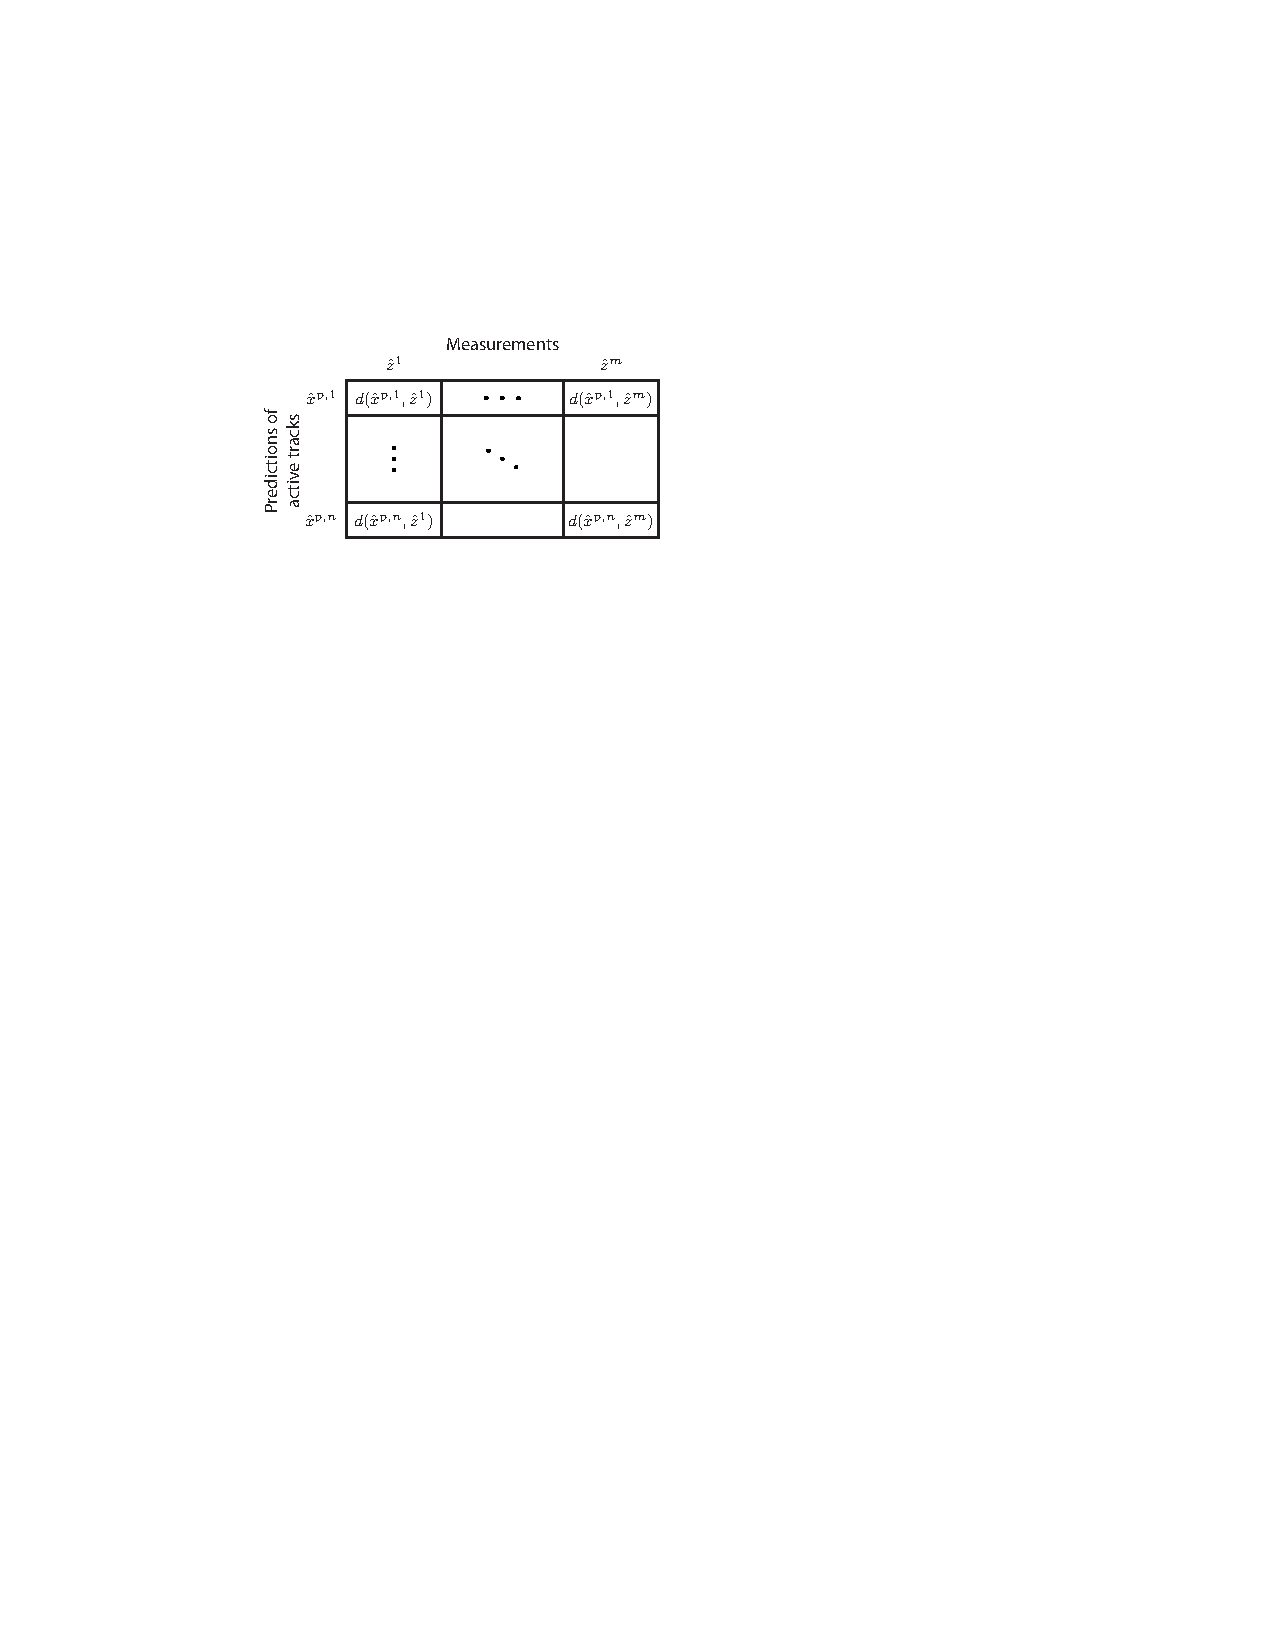
\includegraphics[width=0.6\textwidth]{figures/asso matrix small.pdf}
\caption{Matrix used for the determination of the association decisions. The value in each block is the squared Mahalanobis distance between a measurement and a prediction \cite{pfaff2019multitarget}.}
\label{association matrix simple}
\end{figure}



\subsection{Track Management}

In the optical sorting tasks, particles appear at the start of the observation area and disappear at end start of the observation area. According to \cite{mahler2007statistical}, we can define three states of a track. The first one is \textit{existing} that means a track is extending in the tracking area and should be assigned with a measurement. All the tracks in Figure \ref{association matrix simple} belong to this state. The second one is \textit{appearing} that represents a track is first observed in this timestep. In this case, the new measurement is not assigned to a existing track and should be used for the initialization of the new track. The last one is \textit{disappearing} that means a track is extending out of the tracking area. No measurements is assigned to a disappearing track.

In order to deal with the appearing and disappearing tracks, the extended association matrix is used in the association algorithm, as illustrated in Figure \ref{association matrix}. Except for the cells filled with squared Mahalanobis distances that indicate the distance between each measurement and prediction same as in Figure \ref{association matrix simple}, the other cells of the extended association matrix are filled with distance-like penalty terms that showing the likelihoods of the tracks appearing and disappearing. In this thesis, the association problem is also solved with the GNN \cite{pfaff2019multitarget}. As mentioned in Equation \eqref{likelihood}, it means the likelihood of the association decision from the GNN is maximized. The associated track–measurement pairs can be represented with the indices of the selected cells in the association matrix.



\begin{figure}[htb]
\centering
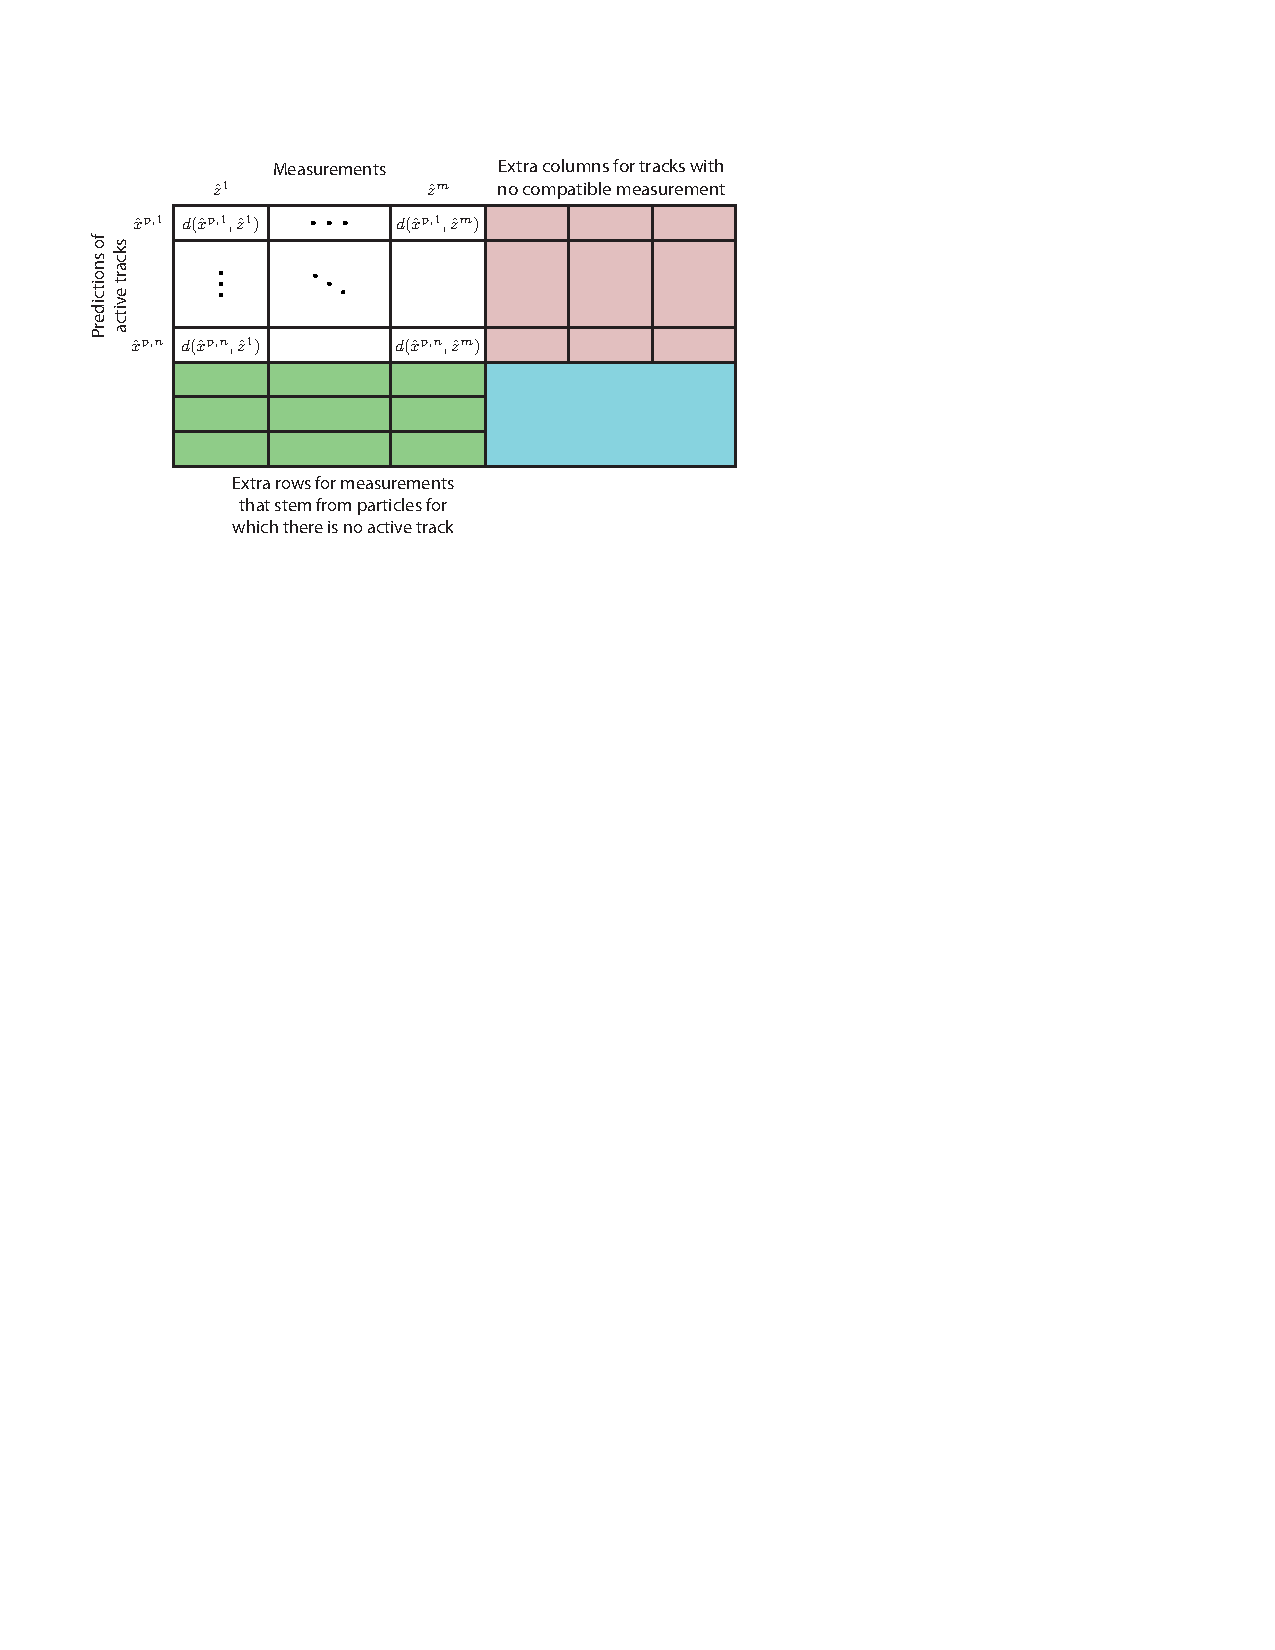
\includegraphics[width=0.8\textwidth]{figures/asso matrix.pdf}
\caption{The extended association matrix used in the implementation of the multitarget tracking algorithm. The areas with different colors represents different state of measurements and tracks \cite{pfaff2019multitarget}.}
\label{association matrix}
\end{figure}


The upper left area includes the squared Mahalanobis distance between each measurement and prediction. When the blocks appear in the result of the LAP, the corresponding measurements are assigned to existed tracks. The size of the upper left area is $m\times n$, where $m$ is the number of active tracks and $n$ is the number of measurements. 
% This area is filled with the squared Mahalanobis distance between each new measurements and predictions of active tracks, as suggested in Equation \eqref{likelihood}.

If the blocks from the upper right area and the bottom left area appear in the result of the LAP, it means respectively the cases of tracks disappearing or appearing. The number of extra columns and rows can be set manually. When this number is higher, the tracking system can deal with more newly appearing tracks. However, using more columns and rows than necessary will cause higher run times, since the problem size of the LAP is larger. 

These two areas dealing appearing and disappearing tracks are filled with distance-like penalty terms. These penalty values represent the probabilities for track appearing and disappearing. When these penalty terms are lower, the tracks or measurements are more possible in this state. In other words, the corresponding cells are more easily to be chosen in the association decision from the GNN algorithm. However, the probabilities for track appearing and disappearing vary at different parts of the belt, as illustrated in Figure \ref{association along belt}. For example, tracks are more possible to appear at the start of the tracking area, but less possible to appear in the middle. Therefore, the value of penalty terms should be a function of the position in the tracking area. In this thesis, the different values of penalty terms are realized with a step function, which gives different penalty terms at different parts of the tracking area. Therefore, two values for penalty terms of track appearing and two for track disappearing are needed. In order to fit the values in the upper right area, the value of those terms should change with different tracking settings, such as belt velocity, particle density on the belt and the noise level in the tracking. The boundary of different tracking area is determined by the product of the initial velocity guess and the additional safety margin coefficient, which are also the hyperparameters in this thesis.

The cells in the blue area in Figure \ref{association matrix} are also filled with penalty terms. The cells in this area are included in the association decision when the extra rows or columns are more than necessary. This probability is not related to the tracking area, so the penalty term here remains the same in the tracking. All the penalty terms as well as the boundary between different tracking phases are considered as hyperparameters in this thesis. These association hyperparameters are listed in Table \ref{List of association hyperparameters}. 

% \textcolor{red}{I have read a document stating that all quantities and variables should be in italic and all units and descriptive terms should be in roman, so I changed all subscripts in the table below into roman even if there is only one letter, like $d_{\mathrm{n}}$}

% \textcolor{red}{This paragraph is small, but also has no relation to the other paragraphs, so it seems strange to merge it into other paragraphs.}

\begin{table}[htbp] 
\small
    \centering
    \caption{List of association hyperparameters.} 
    \label{List of association hyperparameters}
    \begin{tabular}{ccc} 
    \toprule 
    Hyperparameters&Notation&Use\\ 
    \midrule 
    Distance appear at start &$d_{\mathrm{as}}$&For green blocks in Figure \ref{association matrix} in the start phase\\
    Distance appear at middle &$d_{\mathrm{am}}$&For green blocks in Figure \ref{association matrix} in the other phases\\
    Distance disappear at end &$d_{\mathrm{de}}$&For red blocks in Figure \ref{association matrix} in the end phase\\
    Distance disappear at middle &$d_{\mathrm{dm}}$&For red blocks in Figure \ref{association matrix} in the other phases\\
    Distance no change &$d_{\mathrm{n}}$&For blue blocks in Figure \ref{association matrix}\\
    \multirow{2}*{Starting phase coefficient}&\multirow{2}*{$l_{\mathrm{s}}$}& The coefficient determining the boundary\\
    &&between starting and middle phase\\
    \multirow{2}*{Ending phase coefficient}&\multirow{2}*{$l_{\mathrm{e}}$}& The coefficient determining the boundary\\
    &&between middle and end phase\\
    \bottomrule 
    \end{tabular} 
\end{table}

\begin{figure}[htb]
\centering
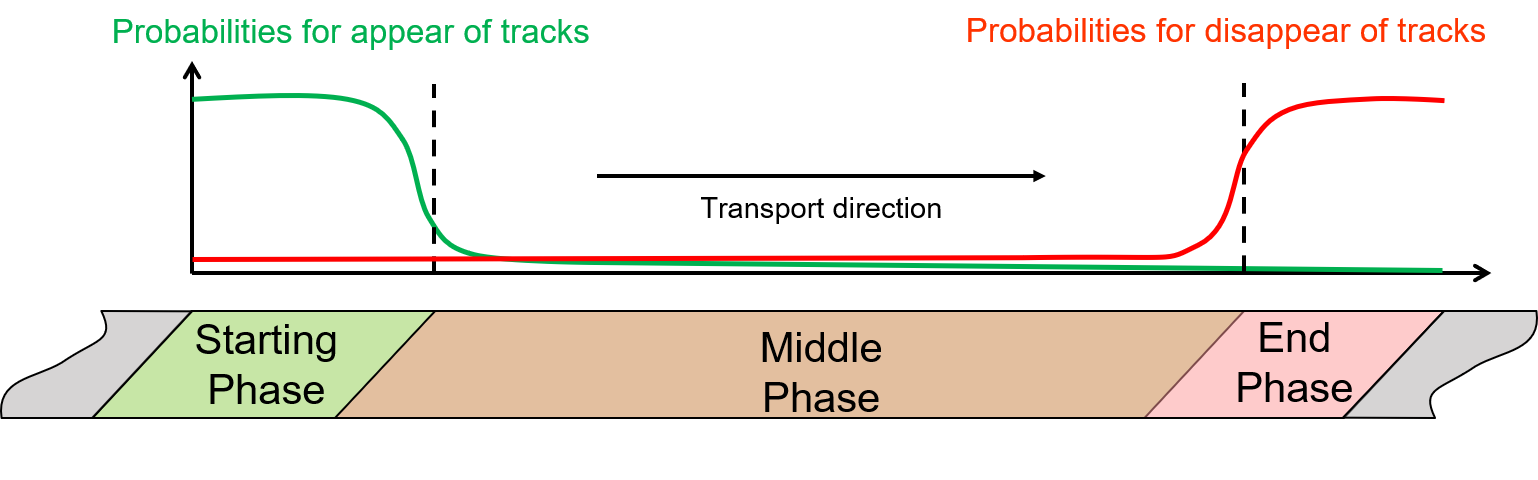
\includegraphics[width=0.8\textwidth]{figures/association along belt.png}
\caption{Probabilities that a new track observed or a track disappeared, adapted from \cite{pfaff2019multitarget}.}
\label{association along belt}
\end{figure}


The appearing tracks from the data association phase need to be initialized for the prediction of the next timestep. In both motion models mentioned in \Sec{Motion Models}, the initial position is initialized as the new measurement. The initial velocity along the transport direction is determined with the initial guess provided by the user at the start of the tracking process. Since this guess is only an inaccurate guess of the initial velocity, this guess is only used in the start of tracking and accompanied with a high variance. After having enough measurements, the initial velocity is refined with the average velocity of the observed particles in every timestep. The list of the initial variances are presented in \Tab{list hp cv} and \ref{list HP cva}. 
% These values can have an effect on tracking accuracy.

Because of errors in image processing, particles can be missed in some timesteps, and the tracks can be interrupted in the middle of the tracking area. To reduce this error, track scores are introduced in the tracking algorithm. Each new track is initialized with a start track score. When the track is associated with a measurement, the track extends normally and the track score increases. When the track has no measurement associated, the track is not regarded as ended immediately, but the track score decreases. Only until the track score is less than a threshold, the track is considered as ended and no longer participate the association .

Until now, we have figured out all the hyperparameters we need to optimize and summarized all the optimization and classification methods we need. In following chapters, we will introduce the operation details of the optimization, including the dataset we use, the configuration of the optimization methods and the optimization results.






























    % \input{4 opt 1}
    % \input{5 opt 2}
    \chapter{Data Collection and Generation}

This chapter introduces all the data used in this thesis. There are three types of data in this thesis. 
% \textcolor{red}{I used "homogeneous materials" instead of "single material", is it all right?}
The first set of datasets that based on the real homogeneous materials were taken from Hornberger's work. These recordings were made with the \textit{TableSort} bulk material sorter at Fraunhofer IOSB, which were then converted into the proper data format over several steps \cite{hornberger2018}. Another dataset with mixtures of construction wastes was also recorded with the \textit{TableSort} sorter. These two sets of datasets are primarily used in the optimization of the hyperparameters for the motion prediction part.
In addition, there are data sets that have been generated through simulations using the discrete element method (DEM). This set of data is mainly used in the optimization of the hyperparameters for the association.
There are also some generated datasets for the validation of the optimization methods.
This chapter will explain the collection or generation process as well as the post-processing of these datasets. The form of the datasets given in the experiments will also be presented in the latter part.

\section{Datasets from Homogeneous Real Materials}

The datasets from homogeneous real materials were recorded with four different bulk materials on the conveyor belt: spheres, peppercorns, cylinders and wheat grains, as illustrated in Figure \ref{fig:schuettgueterSchuessel}. Each dataset contains only one type of material.

\begin{figure}[htbp]
	\centering
	\begin{subfigure}[t]{0.4\textwidth}
		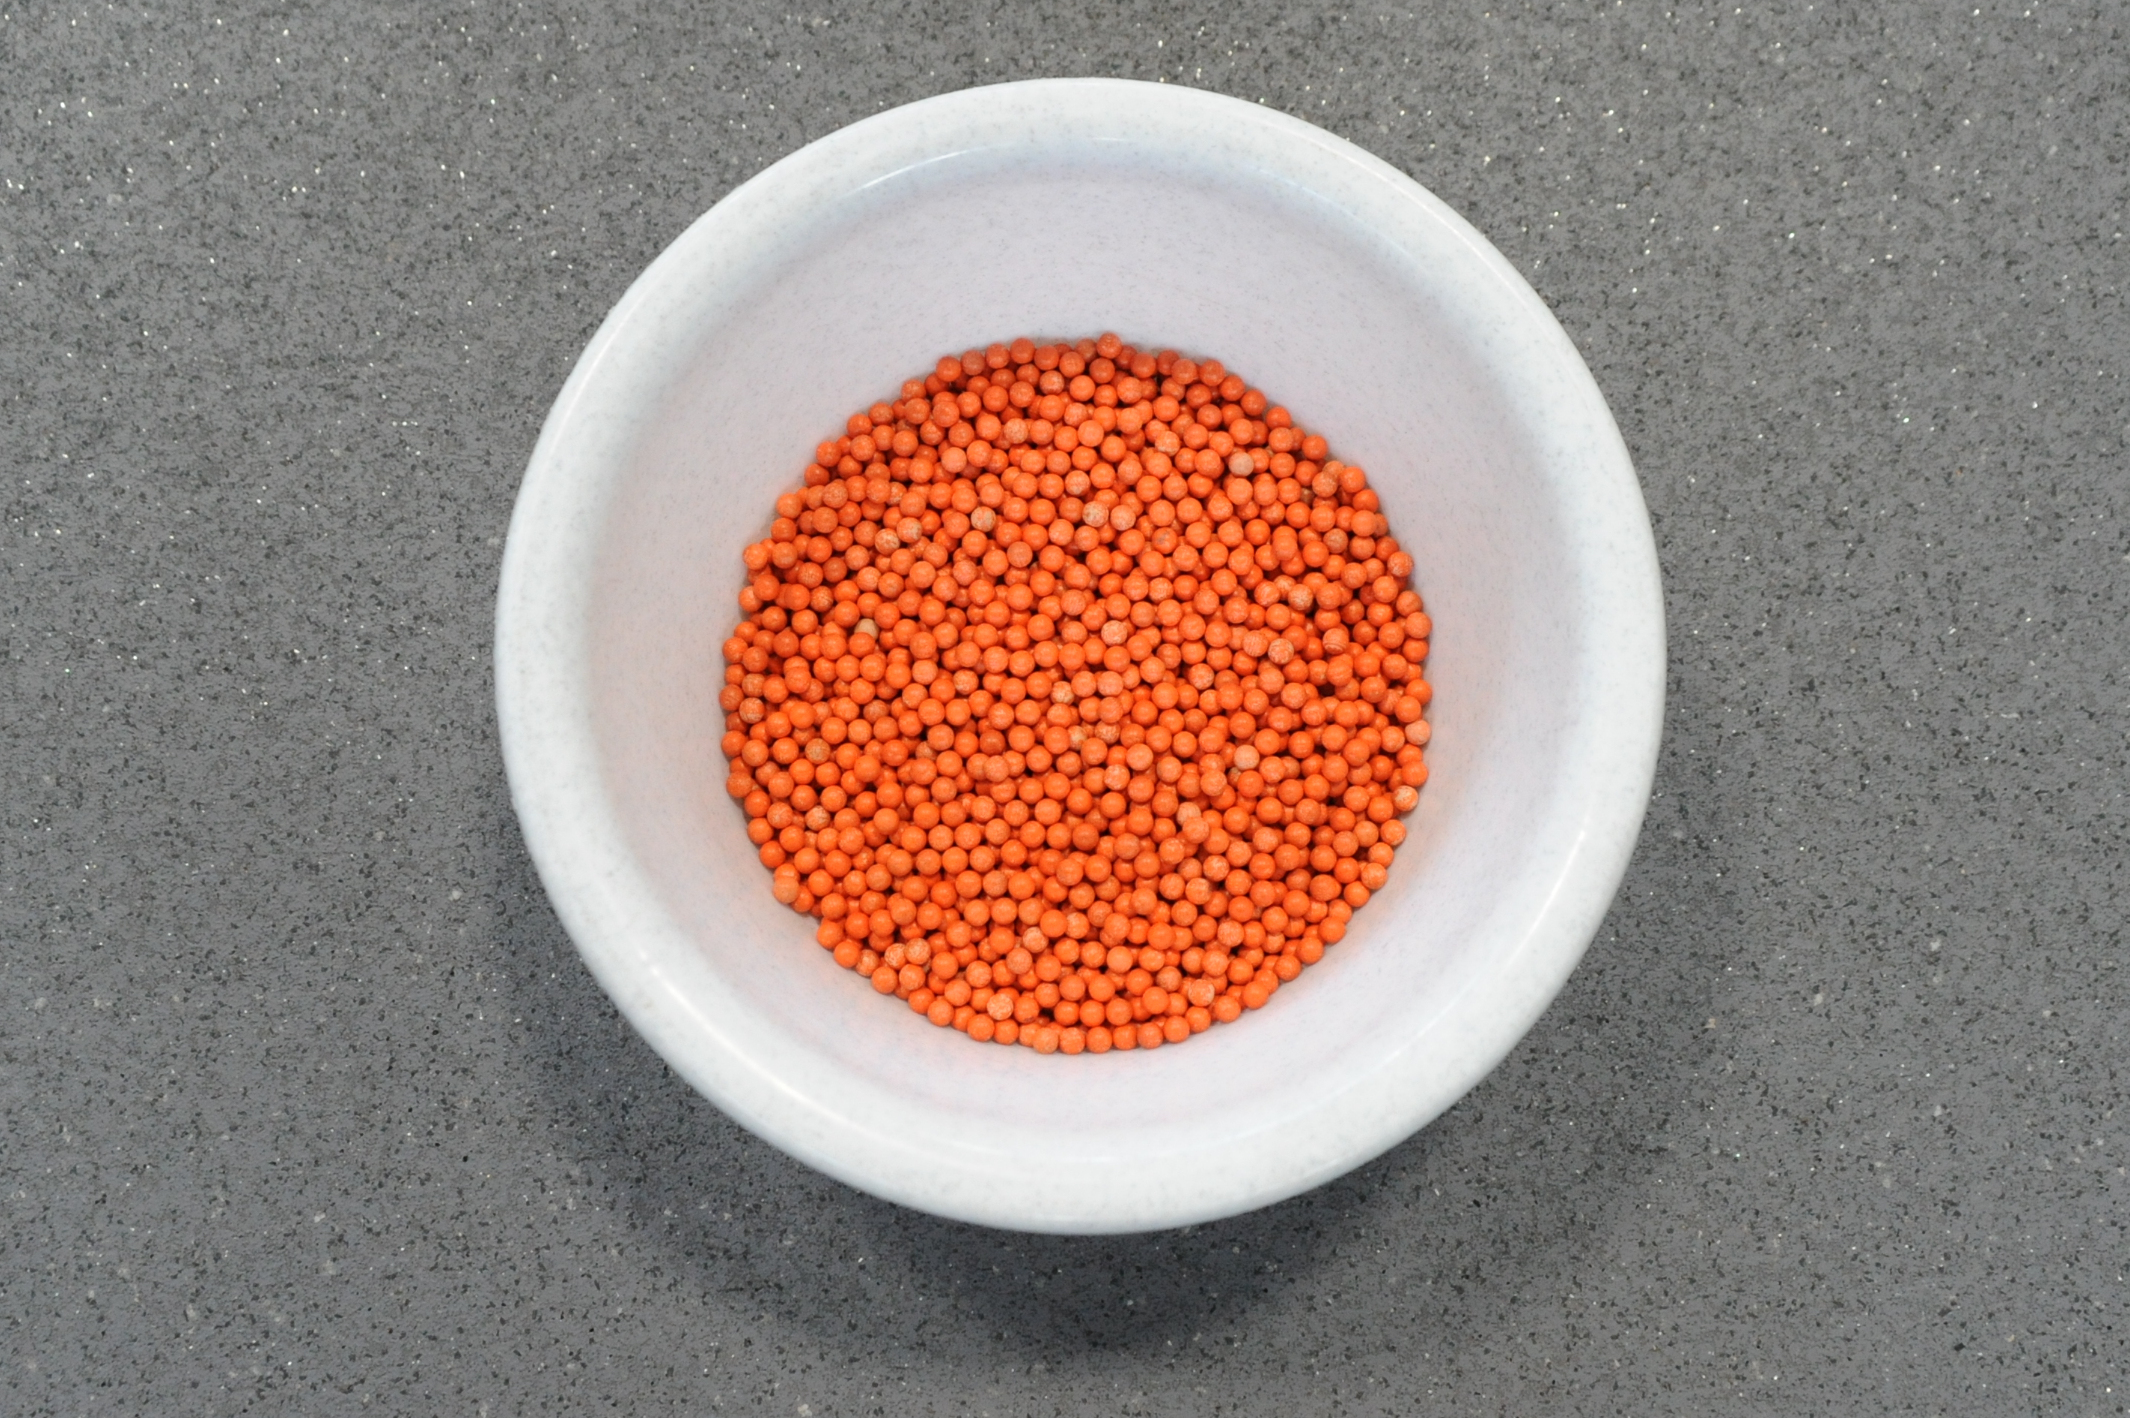
\includegraphics[width=\textwidth]{KugelnCropped2}
		\caption{Spheres}
	\end{subfigure}
	% \hfill
	\quad
	\begin{subfigure}[t]{0.4\textwidth}
		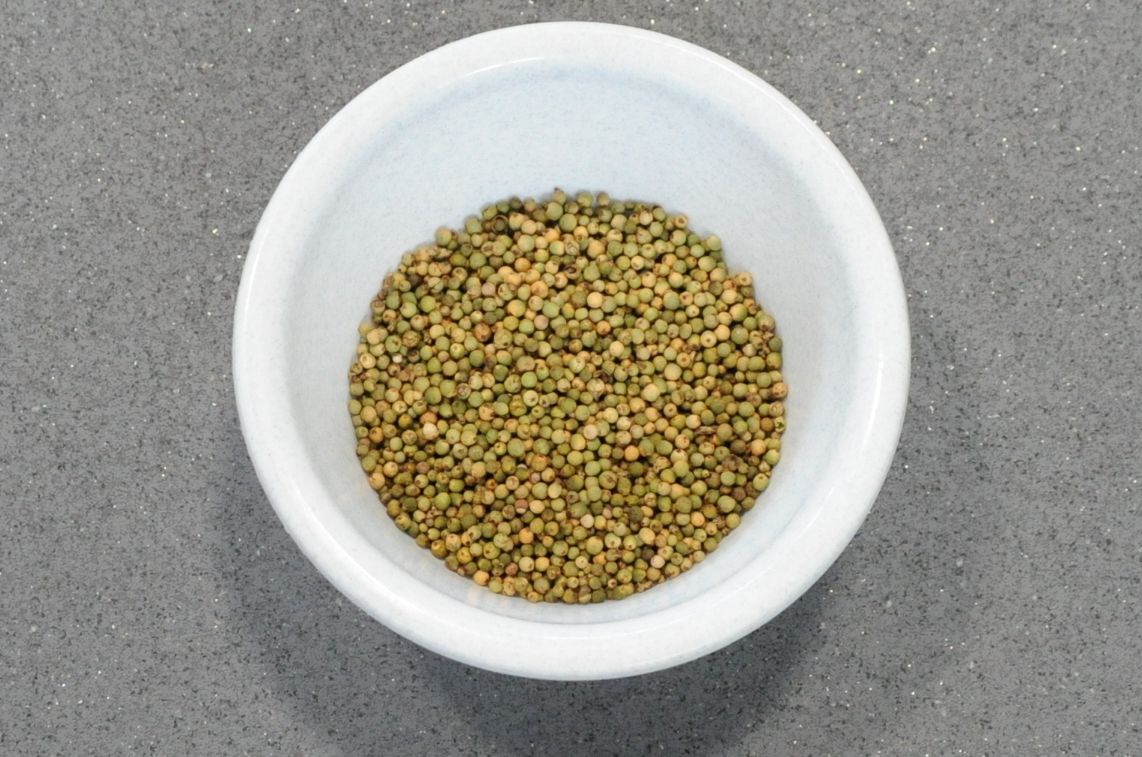
\includegraphics[width=\textwidth]{PfefferCropped2}
		\caption{Peppercorns}
	\end{subfigure}
	\vskip\baselineskip

	\begin{subfigure}[t]{0.4\textwidth}
		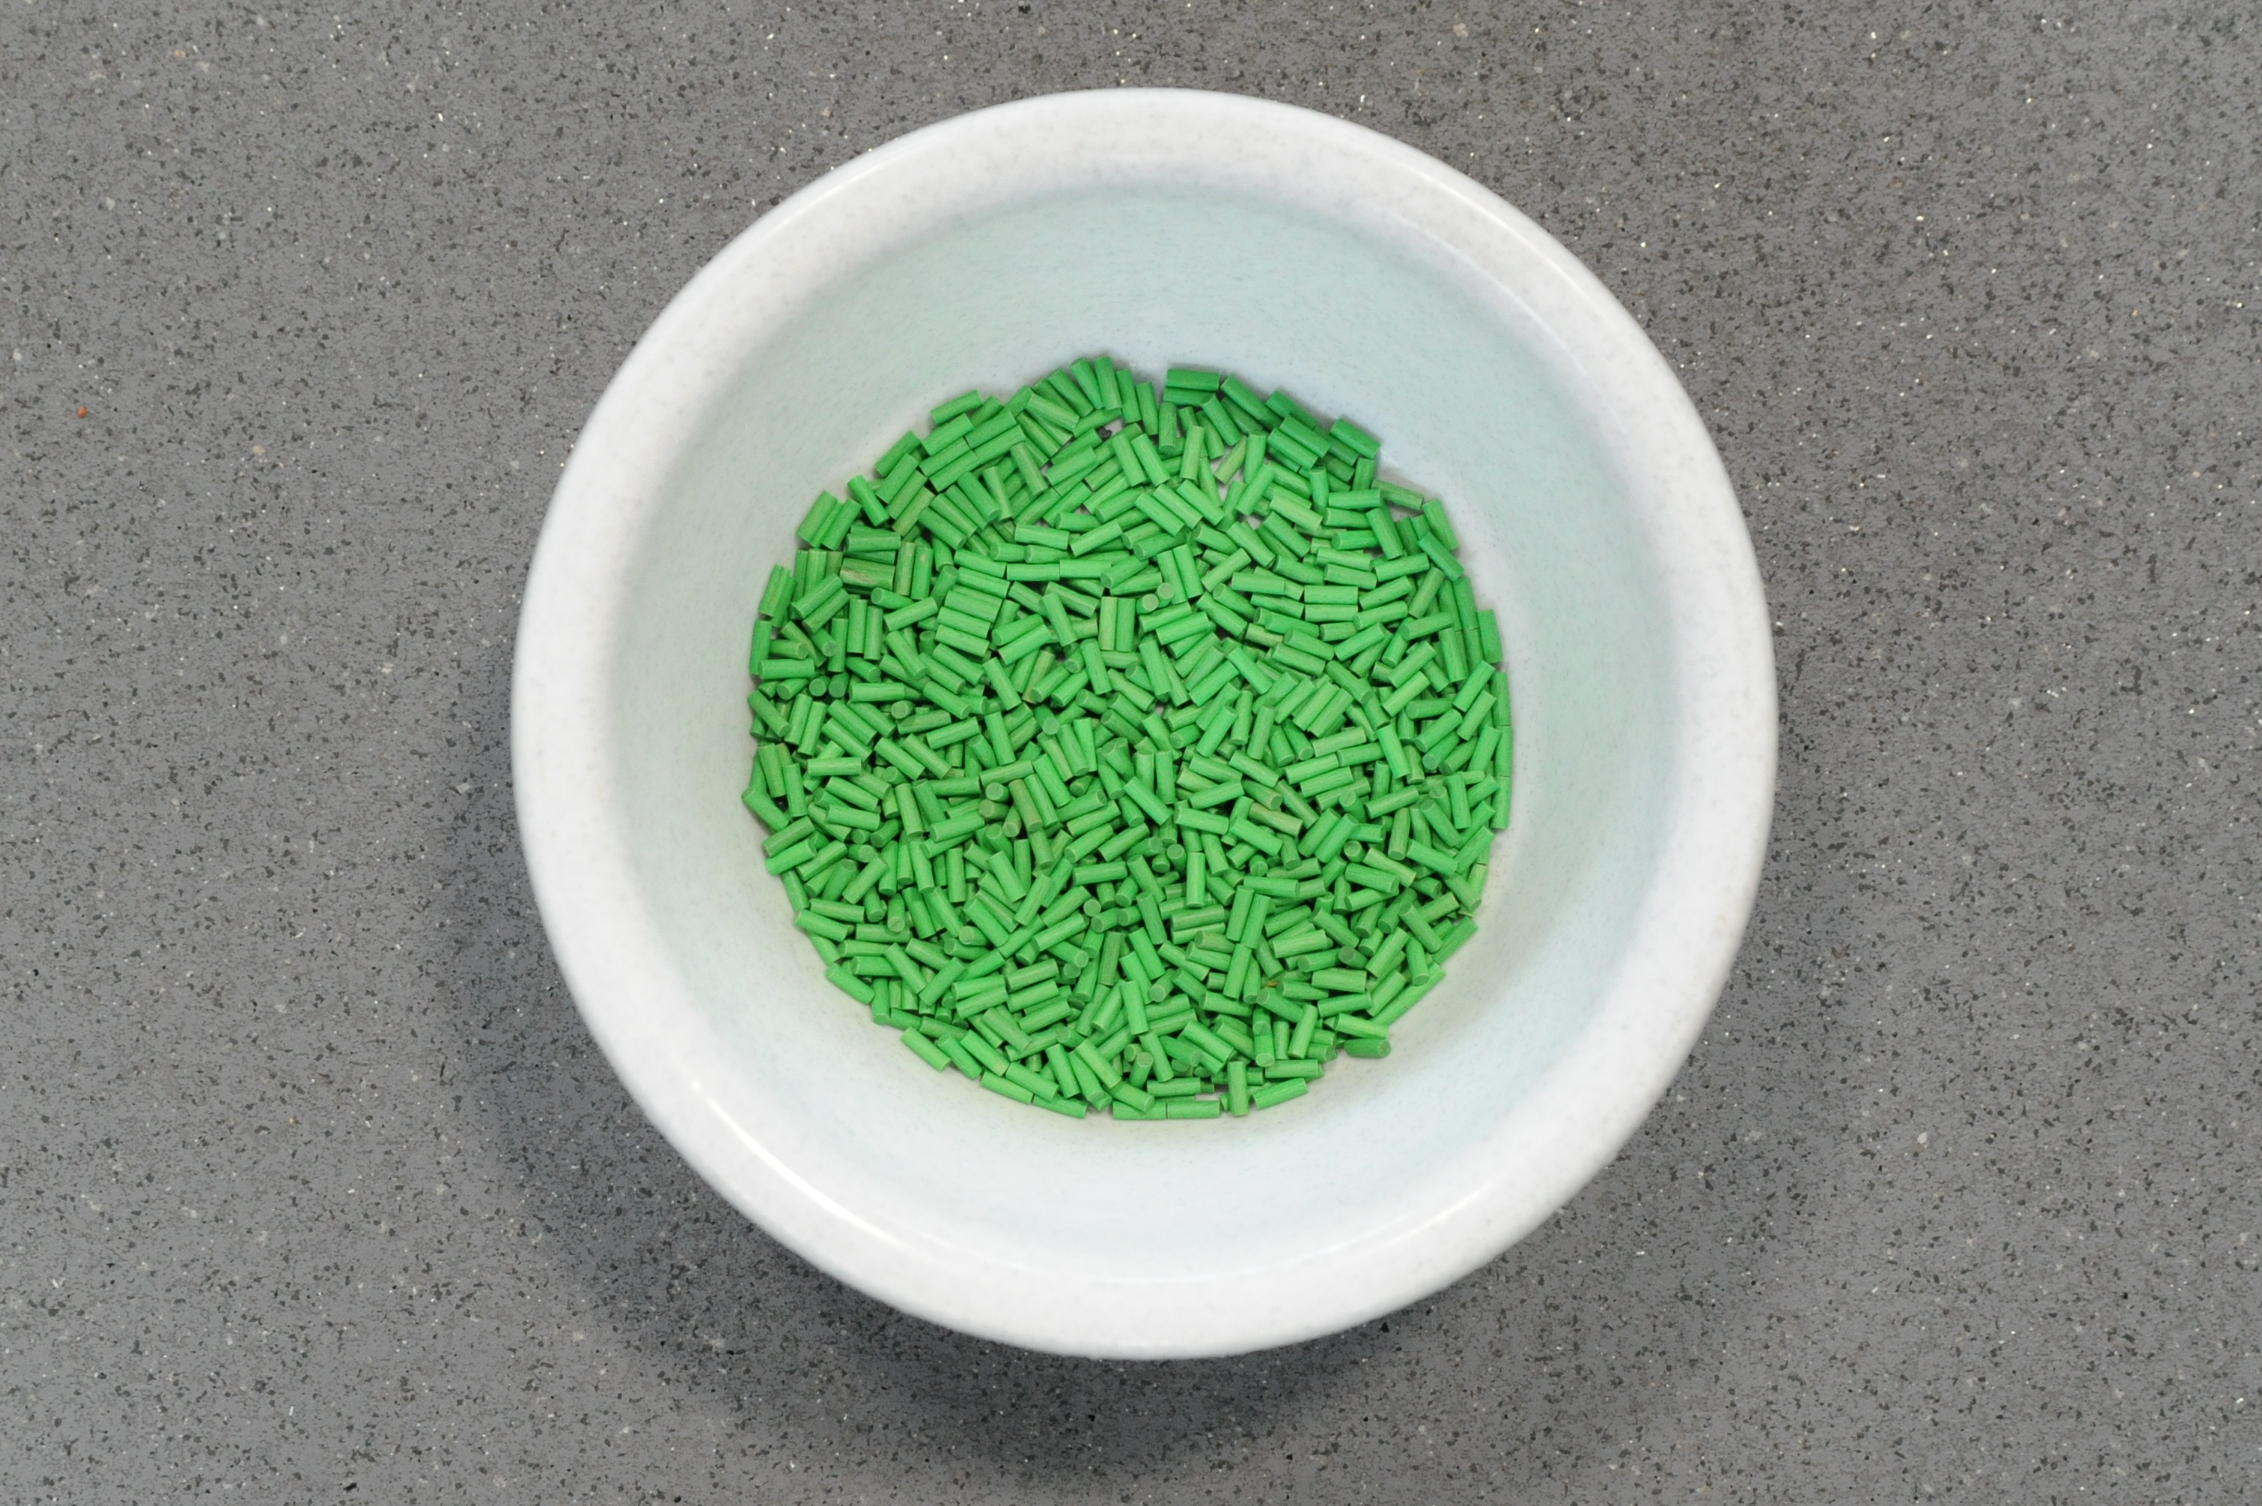
\includegraphics[width=\textwidth]{ZylinderCropped2}
		\caption{Cylinders}
	\end{subfigure}
	\quad
	\begin{subfigure}[t]{0.4\textwidth}
		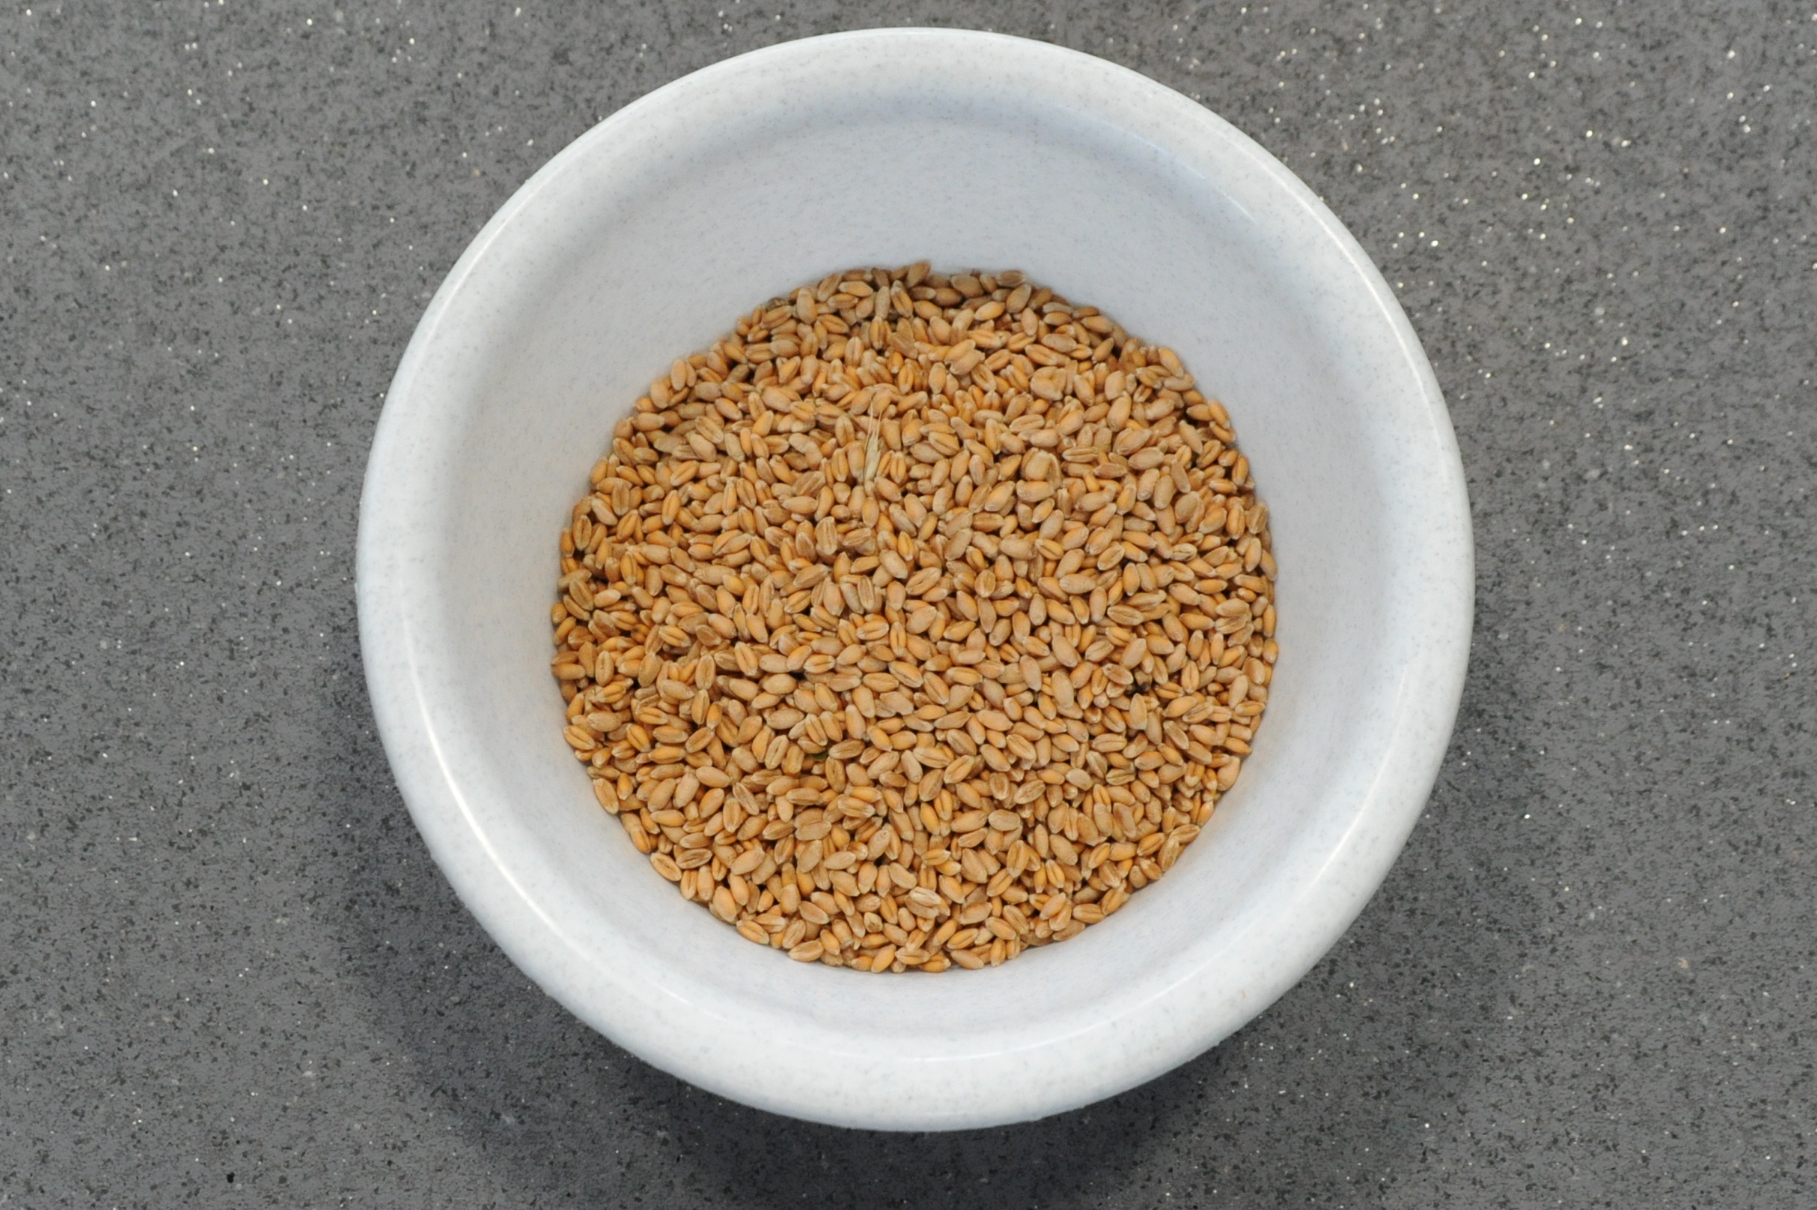
\includegraphics[width=\textwidth]{WeizenCropped2}
		\caption{Wheat grains}
	\end{subfigure}
	\caption{Different materials in the dataset \cite{hornberger2018}.}
	\label{fig:schuettgueterSchuessel}
\end{figure}

As shown in Figure \ref{fig:tablesortsystem}, the camera was assembled above the conveyor belt. The pictures taken by the camera have a resolution of 2320$\times$1726 pixels  \cite{hornberger2018}. Each pixel in the image corresponds approximately to \SI{0.056}{\milli\meter}. The recorded position from the experiment is given in pixels. In the further part of the work, pixels are used as the unit of position for the datasets from real materials.
% average velocity.jpg

The pictures taken in the experiments were later converted into CSV files containing the coordinates of the centers of the particles for each dataset. These CSV files contain the information of measurements in the tracking algorithm. In these CSV files, each line represents an image from a time step. Each line starts with the frame number, followed by the number of particles detected and then the coordinates of the centers of the detected particles. Each coordinate is given in a $1\times 2$ tuple including the coordinate on x-direction $\mathsf{x}$ and y-direction $\mathsf{y}$. In the tracking algorithm, the CSV files are transferred into midpoint matrices, which contain only the coordinate tuples. An example of an excerpt from CSV files can be seen in Table \ref{table:Sample of CSV}. 

% \textcolor{red}{added some information of density, velocity etc.}

The datasets used in this thesis include ten datasets for each material, and each dataset is tested separately in the following experiments. Each dataset contains 3,500 frames. A sphere, peppercorn or wheat grain dataset contains 315\-887 tracks. A cylinder dataset contains 1,101-2,122 tracks. The average velocities of particles in the dataset are between 75-95 pixel/frame. 

The datasets from real materials have no ground truth data. Thus, the last measurement of each track was used for calculating the prediction error. In order to obtain the association information, a reference tracking result was generated with the tracking algorithm from one dataset for each material. The association of each track in the reference tracking result was manually examined to ensure that no association errors appear in the result. Only the dataset with the reference tracking result was used in the grid search for prediction hyperparameters and experiments for association hyperparameters.

\begin{table}[ht]
    \caption{Excerpt from a dataset in .csv format \cite{hornberger2018}.}
	\small
	\centering
    \begin{tabular}{@{}rcrrrrrr@{}}
    \toprule
    Frame   & \#MP & MP\_1\_x  & MP\_1\_y  & MP\_2\_x  & MP\_2\_y  & MP\_3\_x & MP\_3\_y \\ \midrule
    636     & 1    & 1222.9975 & 92.7641   & NaN       & NaN       & NaN      & NaN      \\
    637     & 1    & 1223.4063 & 182.9758  & NaN       & NaN       & NaN      & NaN      \\
    638     & 1    & 1223.6052 & 273.2425  & NaN       & NaN       & NaN      & NaN      \\
    639     & 1    & 1223.7067 & 364.0339  & NaN       & NaN       & NaN      & NaN      \\
    640     & 1    & 1224.0704 & 453.9057  & NaN       & NaN       & NaN      & NaN      \\
    641     & 2    & 1224.2051 & 544.5191  & 1692.4549 & 43.8822   & NaN      & NaN      \\
    642     & 2    & 1224.5793 & 634.7288  & 1696.6901 & 135.9595  & NaN      & NaN      \\
    643     & 2    & 1224.9082 & 726.0094  & 1700.451  & 229.1195  & NaN      & NaN      \\
    644     & 2    & 1225.2296 & 815.9663  & 1704.1472 & 321.2075  & NaN      & NaN      \\
    645     & 2    & 1225.4286 & 906.7078  & 1708.0593 & 414.2785  & NaN      & NaN      \\
    646     & 2    & 1225.7588 & 996.0286  & 1711.5309 & 506.0545  & NaN      & NaN      \\
    647     & 3    & 1226.0411 & 1086.5729 & 1714.8831 & 599.5417  & 961.8821 & 62.7111  \\
    648     & 3    & 1226.2337 & 1175.9271 & 1718.1401 & 691.6325  & 958.5526 & 154.3124 \\
    649     & 3    & 1226.2073 & 1265.7495 & 1721.6618 & 784.5927  & 955.3107 & 246.5241 \\
    650     & 3    & 1226.2543 & 1354.9362 & 1724.9158 & 876.7192  & 952.4919 & 338.1123 \\
    651     & 3    & 1226.2634 & 1444.5903 & 1728.3341 & 970.2909  & 949.2896 & 430.9692 \\
    652     & 3    & 1226.0845 & 1533.0901 & 1732.1745 & 1062.4624 & 946.3455 & 522.8667 \\
    653     & 3    & 1225.7319 & 1621.8461 & 1735.8759 & 1155.2937 & 943.3384 & 615.4545 \\
    654     & 2    & 1739.6714 & 1247.1867 & 940.2511  & 707.7306  & NaN      & NaN      \\
    655     & 2    & 1743.4279 & 1339.4146 & 937.2216  & 800.4557  & NaN      & NaN      \\
    656     & 2    & 1747.1525 & 1430.2501 & 934.5311  & 891.7249  & NaN      & NaN      \\
    657     & 2    & 1750.9771 & 1521.8102 & 931.6626  & 984.2284  & NaN      & NaN      \\
    658     & 2    & 1754.1491 & 1612.5565 & 928.7587  & 1076.4749 & NaN      & NaN      \\
    659     & 1    & 925.8463  & 1168.794  & NaN       & NaN       & NaN      & NaN      \\
    660     & 1    & 922.8752  & 1260.7461 & NaN       & NaN       & NaN      & NaN      \\
    661     & 1    & 920.2056  & 1352.8549 & NaN       & NaN       & NaN      & NaN      \\
    662     & 1    & 917.4051  & 1444.3431 & NaN       & NaN       & NaN      & NaN      \\
    663     & 1    & 914.6493  & 1535.5131 & NaN       & NaN       & NaN      & NaN      \\
    664     & 1    & 911.8565  & 1626.5341 & NaN       & NaN       & NaN      & NaN      \\ \bottomrule
    \end{tabular}
    \normalsize
    
    \label{table:Sample of CSV}
    \end{table}


    
\section{Datasets from Mixture of Real Materials}

% \textcolor{red}{added this section}

The mixed materials used in this thesis are the construction waste containing small particles of bricks and limestones, as shown in Figure \ref{bauschutt}. The experimental settings and data format of the datasets with mixed materials are the same as the homogeneous materials. The average velocities of particles in the dataset are around 65 pixel/frame. 
% This value was also set as the initial velocity guess in the tracking algorithm. 
The mixture material dataset contains three datasets, each with 3500 frames. All three datasets were used in this thesis.

\begin{figure}[htbp]
    \centering
	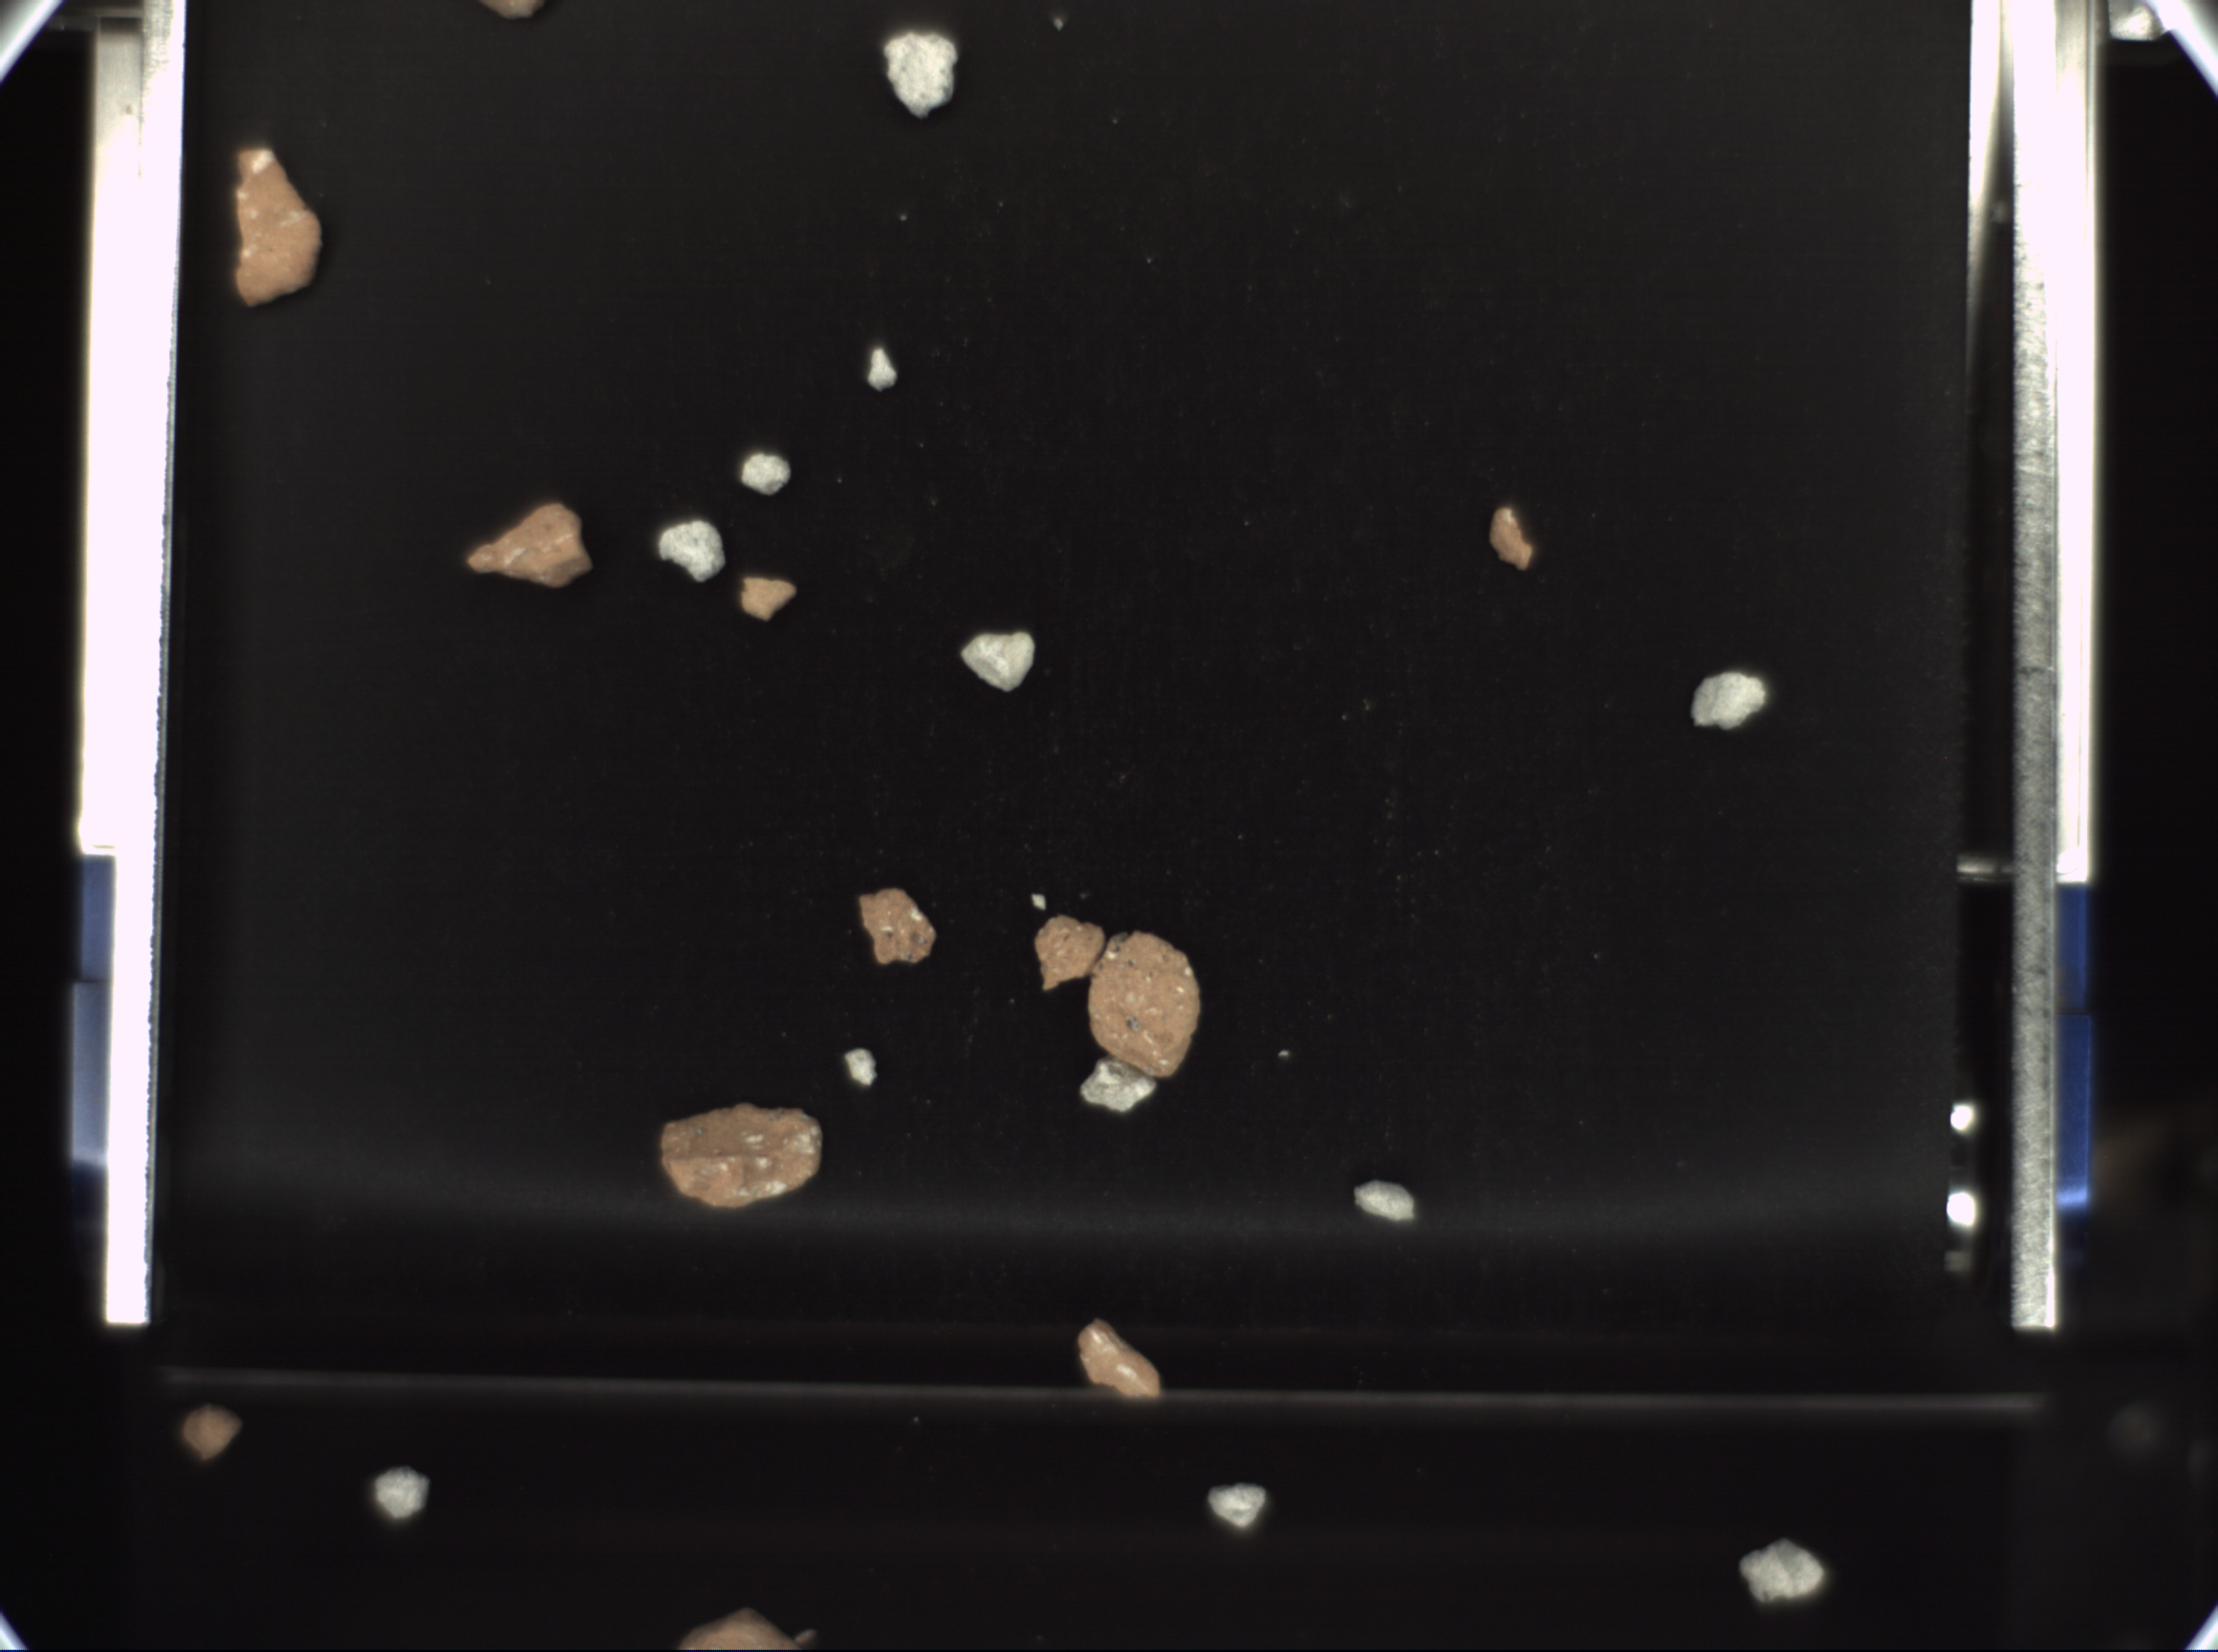
\includegraphics[width=0.6\textwidth]{figures/ZiegelzuKalk50zu50_20gpros00037.png}
	\caption{Mixture of construction wastes, containing particles of bricks and limestones.}
	\label{bauschutt}
\end{figure}


\section{Datasets from Simulation}

In addition to the datasets based on real experiments, some simulated data were also used in this work. \cite{pieper2016numerical} and \cite{pieper2017numerical} show how these datasets were created based on a highly accurate numerical simulation of the \textit{TableSort} system using the discrete element method. The forces acting on the individual particles were calculated numerically based on their condition and the relevant physical laws. Because all the data came from the simulation, the data represent the exact motion of the simulated particles. Thus, all the measurements in the dataset can be seen as the ground truth data and contain no measurement error.

Figure \ref{fig:DEMSimulation} shows the virtual structure of the bulk material sorter on which the simulation was carried out. The position data in the datasets were originally sampled with a frequency of \SI{1000}{\hertz}. However, in order to reduce the size of the dataset and accelerate the tracking process, the frequency was reduced to \SI{100}{\hertz} in the datasets for the experiments in this thesis. The dataset from the simulation is given directly in midpoint matrices in \textsc{Matlab}.

The position information of the simulation is given in meters. The transport direction of the conveyor belt is along the \(\mathsf {x}\) axis. The conveyor belt extends along the \(\mathsf{y} \) axis from \SI{0.0}{\meter} to \SI{0.18}{\meter} and along the \(\mathsf{x}\) - Axis from \SI{0.388}{\meter} to \SI{0.788}{\meter}. The average velocities of particles in the dataset are around \SI{1}{\metre\per\second}, or \SI{0.01}{\metre\per}/frame. The DEM dataset contains 3,713 tracks in 2,000 frames. 

\begin{figure}[htb]
    \centering
	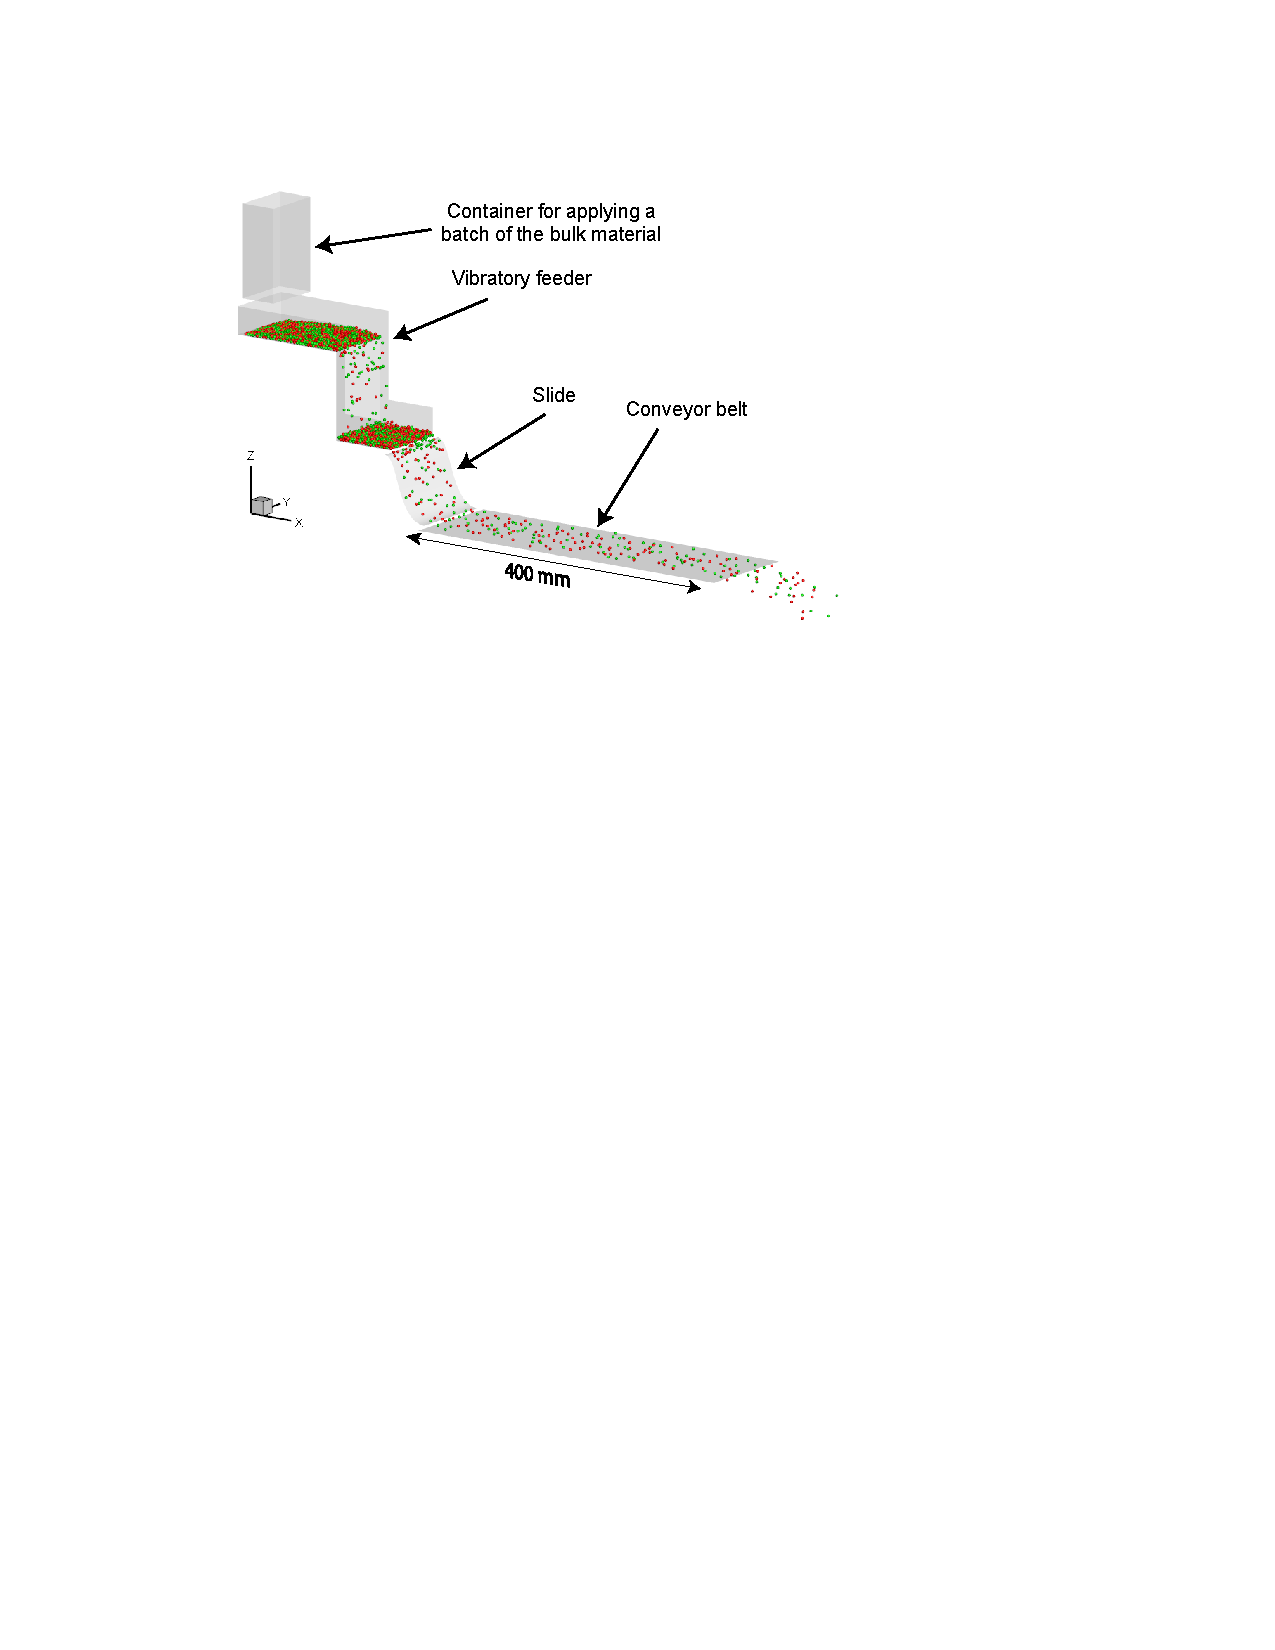
\includegraphics[width=0.8\textwidth]{DEM-Sim}
	\caption{Visualization of the DEM simulation \cite{pfaff2019multitarget}.}
	\label{fig:DEMSimulation}
\end{figure}





\section{Artificial Datasets}
\label{Artificial Datasets}

% \textcolor{red}{added details}

Besides the dataset mentioned above, some simple datasets were generated for the validation of the optimization methods. These datasets were generated according to the motion models mentioned in \Sec{Motion Models}. All the hyperparameters, including the initial velocity and the variances for each state variables, were given before the generation of the artificial dataset. In the validation, the optimization algorithm should reconstruct these hyperparameters. The hyperparameter values for the generation of the datasets are listed in Table \ref{defaultCVvali} and \ref{defaultCVAvali}. In order to avoid the interference of the association errors in the validation, the dataset contains only one track at the same time. The dataset contains 10000 tracks in total, where each track contains 20 measurements.

\begin{table}[htbp] 
    \centering
    \caption{List of the value of the hyperparameters in CV model for artificial datasets.} 
    \begin{tabular}{ccc} 
    \toprule 
    Hyperparameters&Notation& Default value\\ 
    \midrule 
    Initial velocity guess              &$v_{0}$&100\\
    Initial position variance           &$S_{\mathrm{pos}}^{\mathrm{ini}}$&0.5\\
    Initial velocity variance           &$S_{\mathrm{vel}}^{\mathrm{ini}}$&0.2\\
    Refined initial velocity variance   &$S_{\mathrm{vel}}^{\mathrm{ini, r}}$&0.2\\
    Measurement variance                &$S^{\boldsymbol{v}}$&0.2\\
    System noise variance               &$S^{\boldsymbol{w}}$&0.1\\ 
    \bottomrule 
    \end{tabular} 
    \label{defaultCVvali}
\end{table}

\begin{table}[htb] 
    \centering
    \caption{List of the value of the hyperparameters in CVA model for generating the artificial datasets.} 
    \begin{tabular}{ccc} 
    \toprule 
    Hyperparameters&Notation& Value\\ 
    \midrule 
    Initial velocity guess              &$v_{0}$&100\\
    Initial position variance           &$S_{\mathrm{pos}}^{\mathrm{ini}}$&0.5\\
    Initial velocity variance           &$S_{\mathrm{vel}}^{\mathrm{ini}}$&0.2\\
    Refined initial velocity variance   &$S_{\mathrm{vel}}^{\mathrm{ini, r}}$&0.2\\
    Initial angle variance              &$S_{\mathrm{ang}}^{\mathrm{ini}}$&0.1\\
    Measurement position variance       &$S_{\mathrm{pos}}^{\boldsymbol{v}}$&0.2\\
    Measurement velocity variance       &$S_{\mathrm{vel}}^{\boldsymbol{v}}$&0.2\\
    Measurement angle variance          &$S_{\mathrm{ang}}^{\boldsymbol{v}}$&0.1\\
    Prediction position variance        &$S_{\mathrm{pos}}^{\boldsymbol{w}}$&0.1\\
    Prediction velocity variance        &$S_{\mathrm{vel}}^{\boldsymbol{w}}$&0.2\\
    Prediction angle variance           &$S_{\mathrm{ang}}^{\boldsymbol{w}}$&0.1\\
    \bottomrule 
    \end{tabular} 
    \label{defaultCVAvali}
\end{table}

% These datasets served only for the validation of the optimization of the hyperparameters for motion prediction.  The optimization for each hyperparameter is performed with ten datasets in the same setting, and the final optimized value is taken as the average of all the ten optimization results.
    \chapter{Methodology and Implementation}

% \textcolor{red}{added a introduction here.}

This chapter gives the introduction of how the optimizations are performed in this thesis for the hyperparameter optimization. In the first section, the evaluation metrics for prediction errors and association errors are given. Then the operation of the optimization methods for prediction hyperparameters are introduced, including grid search and Bayesian optimization. In the last section, the robust range of the association hyperparameters are introduced, and the methods for the determination of the robust range are explained.

\section{Evaluation Metrics and Loss Functions}
\label{loss function}

Before the introduction of the optimization operations, we need to define when the hyperparameters are optimized. The evaluation metrics can evaluate the performance of the algorithm with given hyperparameters. For the prediction hyperparameters, the prediction error is served as the objective function in the optimization of the hyperparameters. These hyperparameters are optimized when the prediction error is minimized. For the association hyperparameters, when the association error is zero or below than a threshold, we can say that the values of hyperparameters are acceptable.

\subsection{Prediction Error}
\label{Prediction Error}

The prediction error $E_{\mathrm{p}}$ gives a metric for the accuracy of the motion prediction. The prediction error for each track is defined as the distance between the predicted position $\hat{\underline{x}}^\mathrm{p}_{t} = (\mathsf{x}_{t}^\mathrm{p},\mathsf{y}_{t}^\mathrm{p})^\top$ and the ground truth position  $\underline{x}^{\mathrm{GT}}_{t} = (\mathsf{x}_{t}^{\mathrm{GT}},\mathsf{y}_{t}^{\mathrm{GT}})$ of the tracked particle in the last timestep of the track. In the real datasets, the new measurements on the last step $\hat{\underline{z}}_{t}$ are taken as the ground truth value. In the DEM dataset the ground truth values are given in the dataset. The prediction error for the $i$th track is calculated according to
\begin{equation}
    d^{\mathrm{Err}}_{i}=\sqrt{(\mathsf{x}_{t,i}^{p}-\mathsf{x}_{t,i}^{\mathrm{GT}})^{2}+(\mathsf{y}_{t,i}^{p}-\mathsf{y}_{t,i}^{\mathrm{GT}})^{2}}.
\end{equation}
\begin{figure}[htbp]
\centering
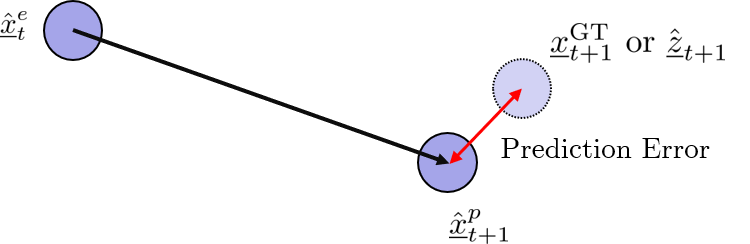
\includegraphics[width=0.6\textwidth]{figures/KF/prediction error.png}
\caption{Definition of the prediction error of a single track.}
\label{prediction error}
\end{figure}


For the whole dataset, the prediction error $E_{\mathrm{p}}$ is defined as the summation of the prediction error of all tracks dividing the number of tracks in the tracking result. The formula of the $E_{\mathrm{p}}$ is given as 
\begin{equation}
    E_{\mathrm{p}} = \frac{\sum_{i=1}^{n} d^{\mathrm{Err}}_{i}}{n}
\end{equation}


At the start and the end of the datasets, there are often some incomplete tracks that start or end in the middle of the tracking area. Because these tracks contain fewer measurements than the other tracks, the tracking accuracy can be also different. In order to reduce the effect of the incomplete tracks, the first and last ten tracks are not included in the calculation of the prediction error. In the optimization, our objection is to find the values of the prediction hyperparameters that minimize the prediction error $E_{\mathrm{p}}$ with the given dataset, as $\underset{\text{hyperparameters}}{\arg\max} E_{\mathrm{p}}(\mathrm{hyperparameters}, \textrm{dataset})$.


\subsection{Association Error}
\label{Association Error}

In the tracking process, each measurement comes from a certain particle. The association process constructs one-to-one correspondences between the tracks and the measurements in each timestep. When the correspondences are different from the real correspondences between particles and measurements, there are association errors. The association error contains errors of the first and second kind. We define the first kind of error as a track including the measurements which should belong to other tracks. An example is depicted in Figure \ref{asso err}b. An error belongs to the second kind of error when is that a measurement is assigned to a wrong track, as illustrated in Figure \ref{asso err}c \cite{pfaff2019multitarget}. 

The first and kind association accuracy rate $A_{a,1}$ and $A_{a,2}$ are defined respectively as the number of the correctly associated tracks or measurements dividing the number of tracks or measurements in the reference tracking result, as
\begin{equation}
    A_{a,1}=\frac{n_{\mathrm{tracks}}^{\mathrm{correct}}}{n_{\mathrm{tracks}}},\quad
    A_{a,2}=\frac{n_{\mathrm{measurement}}^{\mathrm{correct}}}{n_{\mathrm{measurement}}}.
\end{equation}
The harmonic mean association error rate $E_{a}=1-\frac{2A_{a,1}A_{a,2}}{A_{a,1}+A_{a,2}}$ is used in the following part for explaining the general accuracy of the association. The reference tracking result has no association error, and the association result is manually examined, as mentioned in Chapter 4.


\begin{figure}[htbp]
\centering
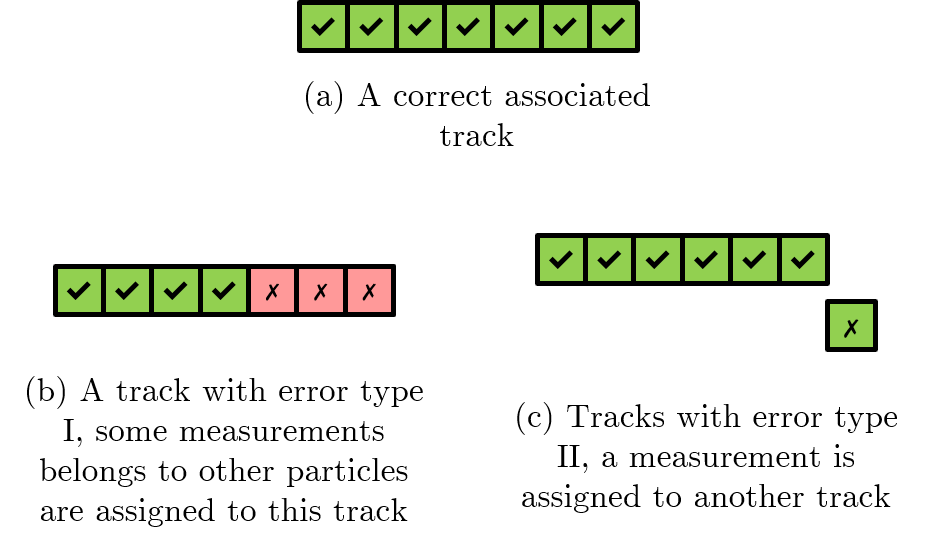
\includegraphics[width=0.7\textwidth]{figures/Asso/association error.png}
\caption{Illustrations for the two types of association errors. The color of the cells indicates the ID of the actual particle from which the measurement stems, adapted from \cite{pfaff2019multitarget}.}
\label{asso err}
\end{figure}

Association errors can be caused by different factors. For example, when two particles collide, the measurements from both particles can exchange to the tracks from another particle, as illustrated in Figure \ref{asso err2}a. Another example is that a particle is assigned to two separate tracks. It can occur when the particle is not observed in some frames, as depicted in Figure \ref{asso err2}b. But even if the measurements are continuous, this type of error can still happen when the prediction is too far away from the measurement or the association hyperparameters are chosen beyond the reasonable range, as shown in Figure \ref{asso err2}c. 

\begin{figure}[htbp]
\centering
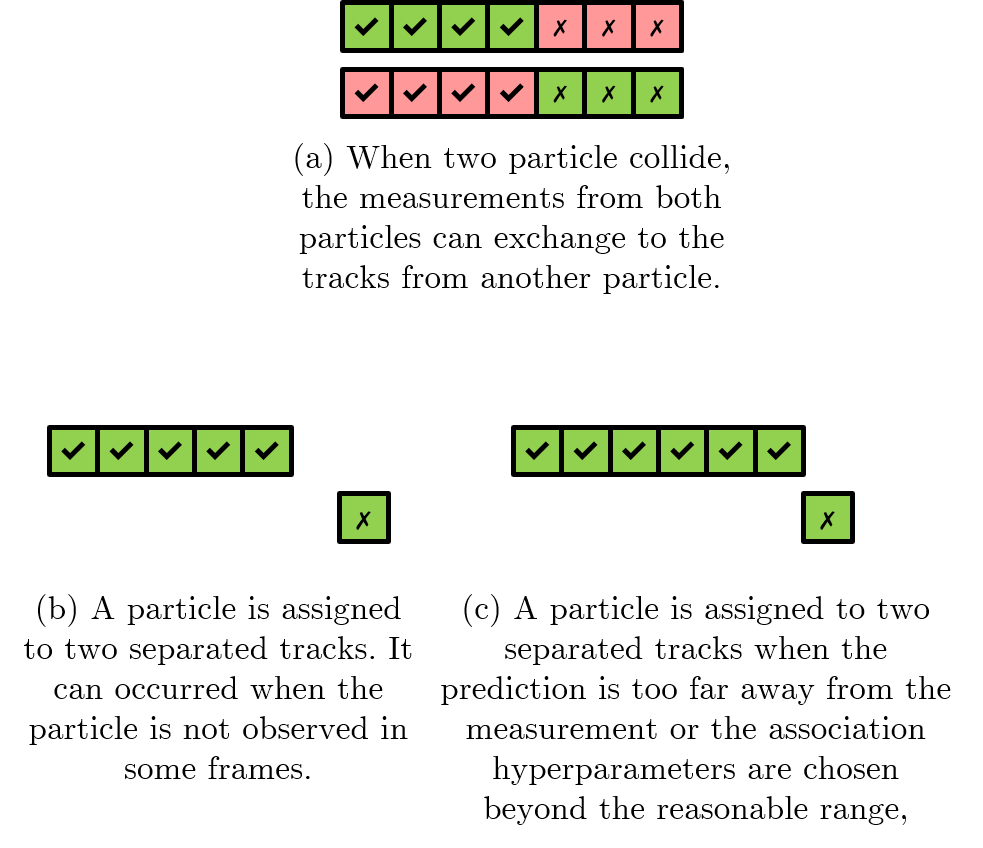
\includegraphics[width=0.7\textwidth]{figures/Asso/association error2.png}
\caption{Illustrations of some typical association errors, inspired from \cite{pfaff2019multitarget}.}
\label{asso err2}
\end{figure}

\section{Optimization of the Hyperparameters of Motion Prediction}  

% \textcolor{red}{added a introduction here. The loss function is also here}

In this section, we introduce the operations for the optimization of the prediction hyperparameters. First, the grid search is applied on the test dataset, for providing an initial knowledge of the effect of the hyperparameters. The hyperparameters and their range for the optimization are also determined with this step. Then, the optimized hyperparameters are obtained with the Bayesian optimization method. The validation method of Bayesian optimization is also introduced in this section. The loss function used in this section is the prediction error $E_{\mathrm{p}}$.

\subsection{Grid Search}

As mentioned in \Sec{gs}, grid search can give us the initial impression of the effect of each hyperparameter. These results can also prompt us for the selection and the range of the hyperparameters in the optimization. In this section, each hyperparameter for prediction was tested with the grid-search-like method. 

All the parameters were checked separately. To avoid the exploding number of searches, only 1-D and 2-D grid searches were performed, which means that only one or two hyperparameters were changed in each set of experiments, and the other hyperparameters remained as the default values. Some of the default values were set as constants, and the others were related to the initial velocity guess. The default values are listed in the Table \ref{defaultCV}, \ref{defaultCVA} and \ref{defaultasso1}. These values were also applied in the Bayesian optimization part for the not optimized hyperparameters.

The test data for the grid search are from the homogeneous material datasets. From each material, only one dataset with the reference result is selected for the grid

\begin{table}[htb] 
    \centering
    \caption{List of the default value of the hyperparameters for CV model.} 
    \begin{tabular}{ccc} 
    \toprule 
    Hyperparameters&Notation& Default value\\ 
    \midrule 
    \multirow{2}*{Initial velocity guess}&\multirow{2}*{$v_{0}$}&100 for homogeneous materials\\
     & & 65 for mixed materials\\
    Initial position variance&$S_{\mathrm{pos}}^{\mathrm{ini}}$&2000\\
    Initial velocity variance           &$S_{\mathrm{vel}}^{\mathrm{ini}}$&$v_{0}/6$\\
    Refined initial velocity variance   &$S_{\mathrm{vel}}^{\mathrm{ini, r}}$&1\\
    Measurement variance&$S^{\boldsymbol{v}}$&2000\\
    System noise variance &$S^{\boldsymbol{w}}$&1\\ 
    \bottomrule 
    \end{tabular} 
    \label{defaultCV}
\end{table}

\begin{table}[htb] 
    \centering
    \caption{List of the default value of the hyperparameters for CVA model.} 
    \begin{tabular}{ccc} 
    \toprule 
    Hyperparameters&Notation& Default value\\ 
    \midrule 
    \multirow{2}*{Initial velocity guess}&\multirow{2}*{$v_{0}$}&100 for homogeneous materials\\
     & & 65 for mixed materials\\
    Initial position variance           &$S_{\mathrm{pos}}^{\mathrm{ini}}$&2000\\
    Initial velocity variance           &$S_{\mathrm{vel}}^{\mathrm{ini}}$&$v_{0}/6$\\
    Refined initial velocity variance   &$S_{\mathrm{vel}}^{\mathrm{ini, r}}$&1\\
    Initial angle variance              &$S_{\mathrm{ang}}^{\mathrm{ini}}$&2\\
    Measurement position variance     &$S_{\mathrm{pos}}^{\boldsymbol{v}}$&2000\\
    Measurement velocity variance &$S_{\mathrm{vel}}^{\boldsymbol{v}}$&$v_{0}/30$\\
    Measurement angle variance      &$S_{\mathrm{ang}}^{\boldsymbol{v}}$&1\\
    Prediction position variance &$S_{\mathrm{pos}}^{\boldsymbol{w}}$&$v_{0}/6$\\
    Prediction velocity variance &$S_{\mathrm{vel}}^{\boldsymbol{w}}$&$v_{0}/60$\\
    Prediction angle variance   &$S_{\mathrm{ang}}^{\boldsymbol{w}}$&0.5\\
    \bottomrule 
    \end{tabular} 
    \label{defaultCVA}
\end{table}

\begin{table}[htb] 
    \centering
    \caption{List of the default value of the association hyperparameters for real materials.} 
    \begin{tabular}{ccc} 
    \toprule 
    Hyperparameters&Notation& Default value\\ 
    \midrule 
    Distance appear at start &$d_{\mathrm{as}}$&0.1\\
    Distance appear at middle &$d_{\mathrm{am}}$&1.5\\
    Distance disappear at end &$d_{\mathrm{de}}$&0.1\\
    Distance disappear at middle &$d_{\mathrm{dm}}$&1.5\\
    Distance no change &$d_{\mathrm{n}}$&0.1\\
    Starting phase coefficient&$l_{\mathrm{s}}$&1.3\\
    Ending phase coefficient&$l_{\mathrm{e}}$&0.5\\
    \bottomrule 
    \end{tabular} 
    \label{defaultasso1}
\end{table}

\FloatBarrier

% \textcolor{red}{added datasets and stepsize here}

search. In order to cover both the high and low values of the hyperparameters, the grid points for searching are set log-likely, as [1, 2, 5, 10, 20,..., 50000, 100000]. According to the default value of the hyperparameters, the search range for position variance is [1, 100000], and the range for other hyperparameters is [0.01, 1000]. 




\subsection{Bayesian Optimization}

% First is the setting of the Bayesian optimization, including parameters and some pre- and postprocedings aside of the optimization algorithm itself. These settings are also applied to the optimization of the real datasets.

% \subsection{Optimization Setting}
% \textcolor{red}{added the parameters for the optimization here}

In order to determine the optimized value of the hyperparameters of motion prediction, the Bayesian optimization method was applied for the optimization. In this part, only the most important hyperparameters were optimized. The hyperparameters for optimization were determined with the result of gird search, respectively the system noise variance $S^{\boldsymbol{w}}$ in the CV model and the prediction position variance $S_{\mathrm{pos}}^{\boldsymbol{w}}$ in the CVA model. The detailed selection process of the hyperparameters for optimization will be presented in the next chapter. In this section, ten datasets from each homogeneous material and all the three datasets from the mixture material were used as the data for the optimization. The objective function for optimization is the prediction error of each dataset.

The optimization was accomplished with the \textit{bayesopt} function in \textsc{Matlab}. The objective function was the prediction error in \Sec{Association Error}. The values of the important arguments for Bayesian optimization are presented in Table \ref{bayopt setting}. The argument \say{ExplorationRatio} is a parameter controlling the ratio of the exploiting and exploring, which have a similar effect with the exploration ratio in \Sec{bayopt intro}. \say{MaxObjectiveEvaluations} determines the iteration number of each optimization. The acquisition function used in the optimization is the expected improvement acquisition function with \textit{Per Second} and \textit{Plus} method. The other arguments remained as default in optimization. These settings applied to all datasets.

\begin{table}[htbp] 
    \centering
    \caption{Settings of the \textit{bayesopt} function.} 
    \begin{tabular}{cc} 
    \toprule 
    Arguments in the \textit{bayesopt} function&Value\\ 
    \midrule 
    \textquoteleft ExplorationRatio\textquoteright           &0.6\\
    \textquoteleft MaxObjectiveEvaluations\textquoteright    &20\\
    \textquoteleft AcquisitionFunctionName\textquoteright    &\textquoteleft expected-improvement-per-second-plus\textquoteright\\
    \bottomrule 
    \end{tabular} 
    \label{bayopt setting}
\end{table}



% \subsection{Clustering}


\section{Robust Range Determination of the Association Hyperparameters}

% \subsection{Robust Range of the Association Hyperparameters}
\label{Robust Range of the Association Hyperparameters}

Different from the hyperparameters of motion prediction, the association hyperparameters have no particular optimized value, but only a robust range. In this thesis, the robust range is defined as the range of the hyperparameters, with which the association error is zero. When the association hyperparameters are taken from this range, the association error will remain zero, even if under different values of the hyperparameters.

Take the association matrix in Figure \ref{asso example} as an example. In this matrix, the two measurements should be assigned to two existing tracks. The distance disappear and appear at middle are set both at 2. Under these circumstances, as long as the distance no change is lower than 3, the association can be correctly performed. Therefore, $[0,3]$ is recognized as the robust range of the hyperparameter distance no change.

\begin{figure}[htbp]
\centering
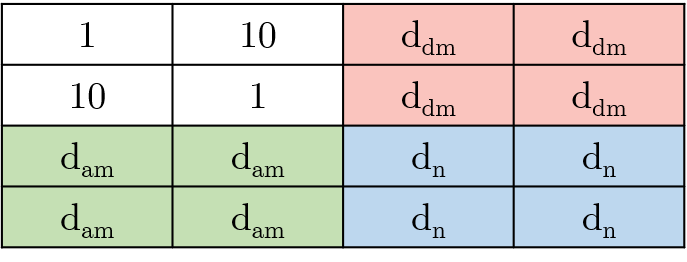
\includegraphics[width=0.4\textwidth]{figures/Asso/association matrix example.png}
\caption{An example of the association matrix.}
\label{asso example}
\end{figure}


\begin{figure}[htbp]
	\centering
	\begin{subfigure}[t]{0.5\textwidth}
		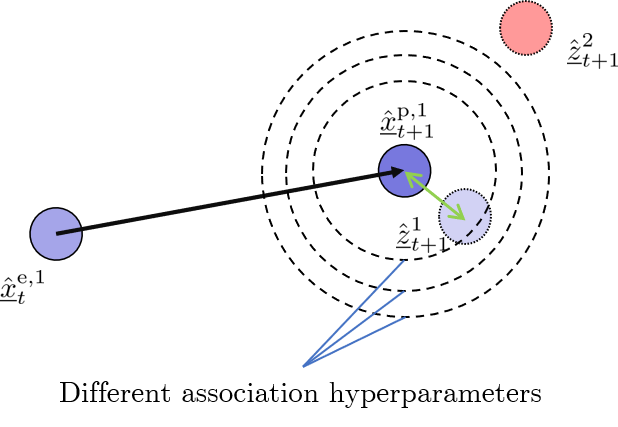
\includegraphics[width=\textwidth]{figures/Asso/robust range1.png}
		\caption{An association without error. The association hyperparameters are in the robust range.}
		\label{robust range1}
	\end{subfigure}
% 	\label{robust range1}
	% \hfill
	\vskip\baselineskip
	
	\begin{subfigure}[t]{0.4\textwidth}
		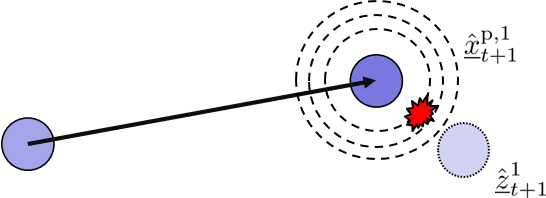
\includegraphics[width=\textwidth]{figures/Asso/robust range2.png}
		\caption{An association error occurred because the bound of association is too low.}
		\label{robust range2}
	\end{subfigure}
	\quad
	\begin{subfigure}[t]{0.3\textwidth}
		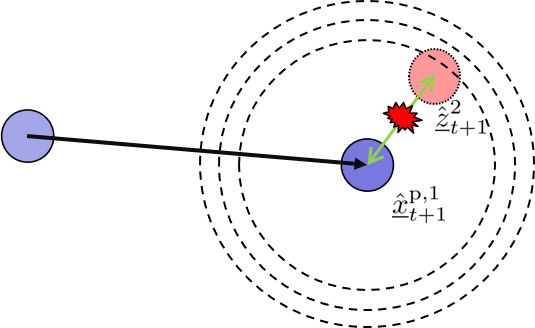
\includegraphics[width=\textwidth]{figures/Asso/robust range3.png}
		\caption{An association error occurred because the bound of association is too high.}
		\label{robust range3}
	\end{subfigure}
% 	\begin{subfigure}[t]{0.4\textwidth}
% 		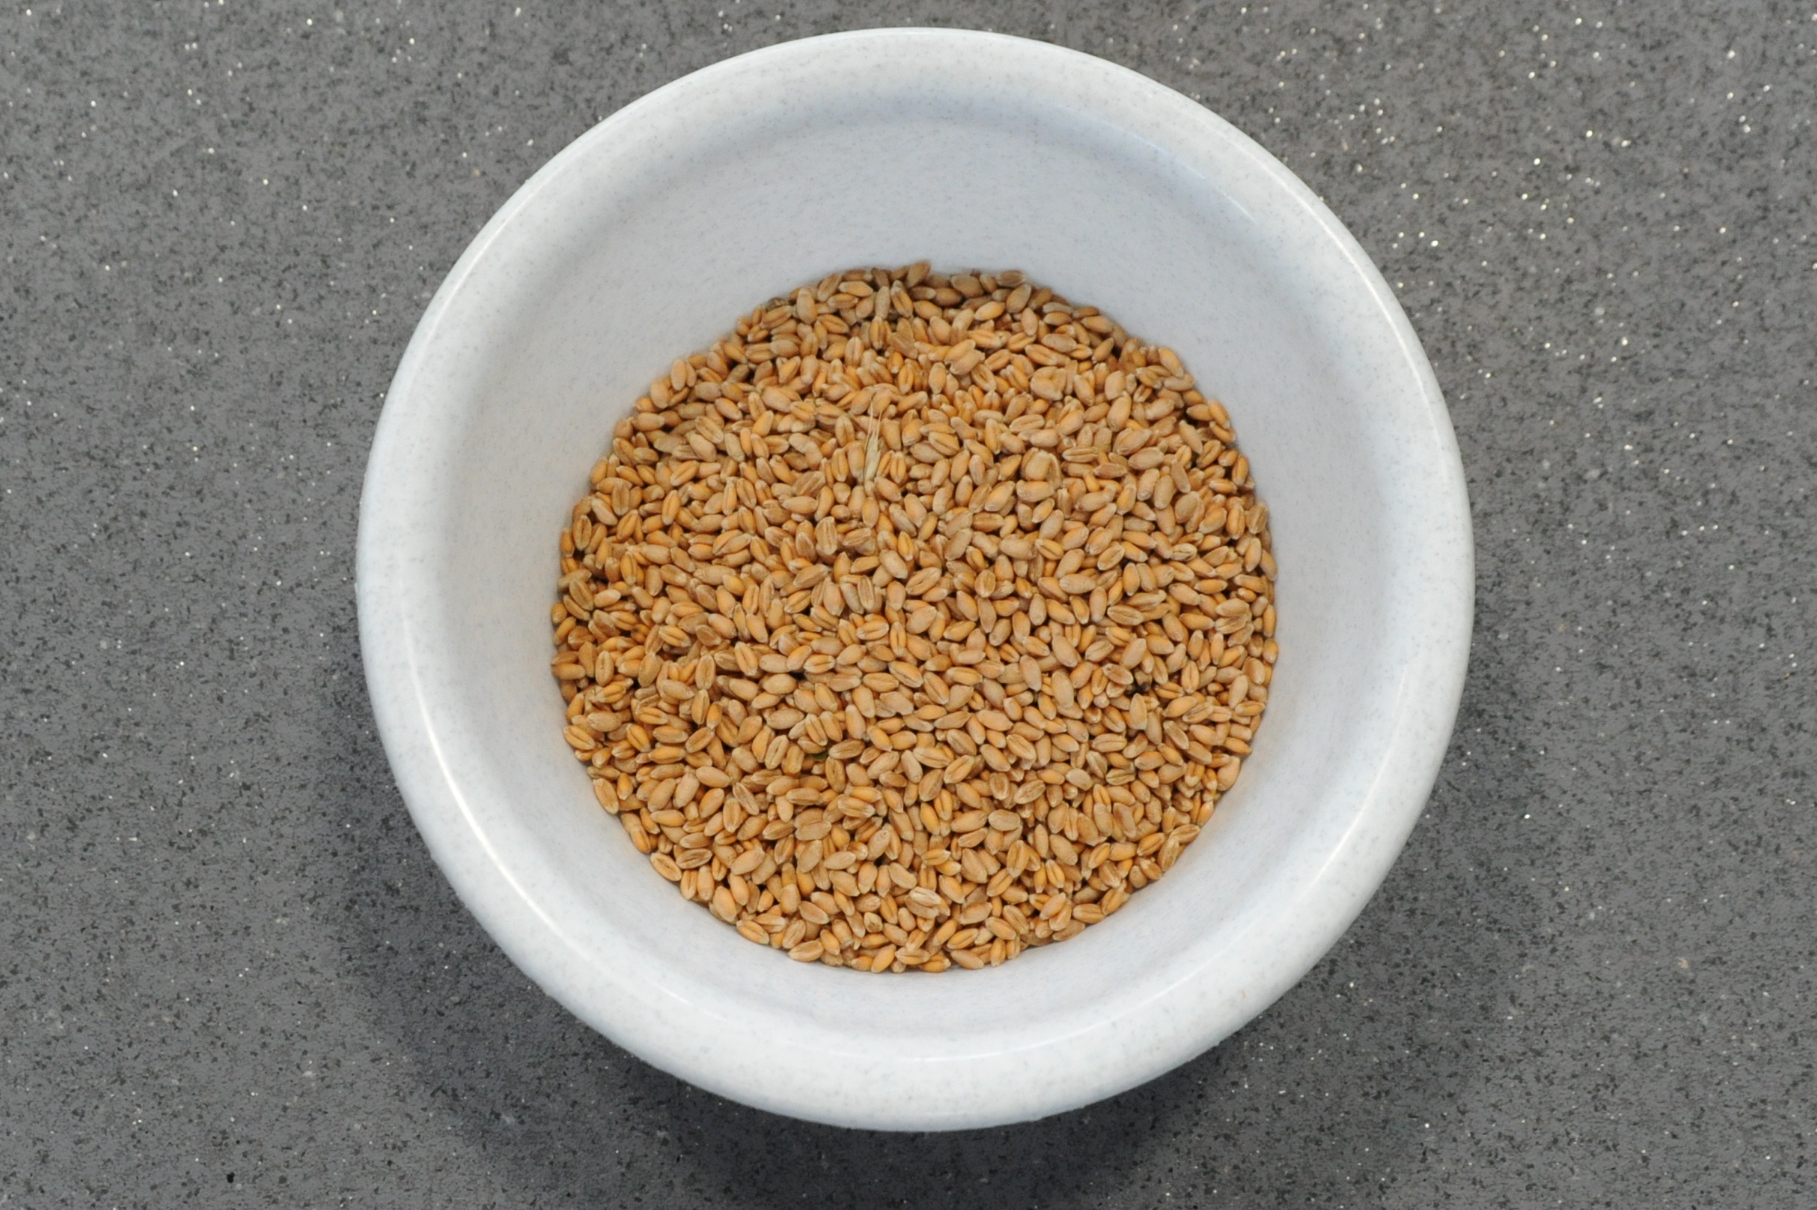
\includegraphics[width=\textwidth]{WeizenCropped2}
% 		\caption{Wheat grains}
% 	\end{subfigure}
	\caption{The effect of the value of the association parameters. When the association hyperparameters are in the robust range, as illustrated in Figure (a), the association can be performed without error, even if the values of the hyperparameters are different, as shown with the different radius of the black dashed circle. However, when the hyperparameters go beyond the robust range, the association error occurs, as illustrated in Figure (b) and (c).}
	\label{robust range}
\end{figure}


In the following part of this thesis, the robust range of the distance-like penalty terms in the association matrix are examined with 1-D grid search and SVM. Because the coefficients for the range of different tracking phases can be directly derived from the analysis of the tracking area, these coefficients are discussed separately.


\subsection{Grid Search}
With grid search, we can figure out the effect of each association hyperparameter on the association error and get a rough estimation of the robust range of each hyperparameter. The grid search is performed with the CVA model in this section where only one association hyperparameter is changed in a set of searches, and the other hyperparameters remain as default values, as shown in Table \ref{defaultCVA2} and \ref{defaultasso2}. The test data for the grid search are from the DEM datasets. The search range is [0, 0.03] with a step size of 0.001.




\begin{table}[htbp] 
    \centering
    \caption{List of the default value of the prediction hyperparameters for DEM datasets.} 
    \begin{tabular}{ccc} 
    \toprule 
    Hyperparameters&Notation& Default value\\ 
    \midrule 
    Initial velocity guess              &$v_{0}$&0.01\\
    Initial position variance           &$S_{\mathrm{pos}}^{\mathrm{ini}}$&$v_{0}/15$\\
    Initial velocity variance           &$S_{\mathrm{vel}}^{\mathrm{ini}}$&$v_{0}/6$\\
    Refined initial velocity variance   &$S_{\mathrm{vel}}^{\mathrm{ini, r}}$&1\\
    Initial angle variance              &$S_{\mathrm{ang}}^{\mathrm{ini}}$&2\\
    Measurement position variance       &$S_{\mathrm{pos}}^{\boldsymbol{v}}$&$v_{0}/15$\\
    Measurement velocity variance       &$S_{\mathrm{vel}}^{\boldsymbol{v}}$&$v_{0}/30$\\
    Measurement angle variance          &$S_{\mathrm{ang}}^{\boldsymbol{v}}$&1\\
    Prediction position variance        &$S_{\mathrm{pos}}^{\boldsymbol{w}}$&$v_{0}/6$\\
    Prediction velocity variance        &$S_{\mathrm{vel}}^{\boldsymbol{w}}$&$v_{0}/60$\\
    Prediction angle variance           &$S_{\mathrm{ang}}^{\boldsymbol{w}}$&0.5\\
    \bottomrule 
    \end{tabular} 
    \label{defaultCVA2}
\end{table}


\begin{table}[htbp] 
    \centering
    \caption{List of the default value of the association hyperparameters for DEM datasets.} 
    \begin{tabular}{ccc} 
    \toprule 
    Hyperparameters&Notation& Default value\\ 
    \midrule 
    Distance appear at start        &$d_{\mathrm{as}}$&0.001\\
    Distance appear at middle       &$d_{\mathrm{am}}$&0.03\\
    Distance disappear at end       &$d_{\mathrm{de}}$&0.001\\
    Distance disappear at middle    &$d_{\mathrm{dm}}$&0.03\\
    Distance no change              &$d_{\mathrm{n}}$&0.0001\\
    Starting phase coefficient      &$l_{\mathrm{s}}$&1.3\\
    Ending phase coefficient        &$l_{\mathrm{e}}$&0.5\\
    \bottomrule 
    \end{tabular} 
    \label{defaultasso2}
\end{table}


\subsection{Data and Setting for the SVM training}
\label{training data svm}

% \textcolor{red}{added more detailed info}
In this section, some SVMs that can give us information about the robust range in higher dimensional hyperparameter spaces are trained. The SVMs can also provide us a model to estimate whether a given set of values of the association hyperparameters are in the robust range. 

The data for the training of the SVMs were generated with the \textit{TrackSort} Algorithm and the DEM dataset. The tracking results were compared with the reference dataset to determine the association error rate. Then these results were binary labeled by whether the association error occurs. The label for each tracking result was recorded along with the association hyperparameters. These hyperparameter tracking error pairs were used as the training dataset of the SVM. 

The training of SVM was performed with 2-D and 5-D training datasets. Each 2-D dataset, where only two hyperparameters were changed and the other hyperparameters remained as default, includes 100 data points for training. The 2-D datasets include each combination of the hyperparameters. The 5-D dataset, where all the five distance-like penalty terms are changed, includes 10,000 data points. The SVM is trained with 10-fold training, where the dataset is divided into 10 folds in equal size. In each training, nine folds of the data points will be the training data and the left fold serves as the test set. The final model is taken from the best result in all 10 training results. All the data were generated with the CVA model, and the prediction hyperparameters for these datasets are shown in Table \ref{defaultCVA2}. The values for the unchanged association hyperparameters with DEM datasets are presented in Table \ref{defaultasso2}. 
% The initial velocity guess for the DEM dataset is set as 0.01.


% \subsection{Setting of the SVM Training}

The training of the SVM was accomplished with the \textit{fitcsvm} function in \textsc{Matlab}. The objective function is the prediction error in \Sec{Association Error}. The values of the important arguments for Bayesian optimization are presented in Table \ref{bayopt setting}. We used the RBF kernel for the SVM. The hyperparameters for the SVM including the penalty factor $c$ and the kernel size $\sigma$ were automatically optimized with Bayesian optimization. The other arguments remained as default. For the 5-D SVMs, we used 10-fold cross-validation. The SVMs provide us classifiers of the hyperparameters that output whether the association error is zero with the given set of hyperparameters. The decision boundary of the SVMs is considered as the robust range of the hyperparameters.

\begin{table}[htbp] 
    \centering
    \caption{Settings of the \textit{fitcsvm} function.} 
    \begin{tabular}{cc} 
    \toprule 
    Arguments in the \textit{fitcsvm} function&Value\\ 
    \midrule 
    \textquoteleft KernelFunction\textquoteright             &'rbf'\\
    \textquoteleft OptimizeHyperparameters\textquoteright    &'auto'\\
    \multirow{2}*{\textquoteleft HyperparameterOptimizationOptions\textquoteright}&struct(\textquoteleft AcquisitionFunctionName',\\
     & \textquoteleft expected-improvement-plus'))\\
    \textquoteleft KFold\textquoteright&                  10\\
    \bottomrule 
    \end{tabular} 
    \label{svm setting}
\end{table}

 
    \chapter{Result and Evaluation}

In this chapter, the results of the optimized prediction hyperparameters and the robust range of the association hyperparameters are presented. In \Sec{1d}, the effects of all tracking hyperparameters are first examined with grid search. The effects of some hyperparameters are explained, and the most effective hyperparameters and their range for the optimization are also presented in this section. In \Sec{validation}, the Bayesian optimization method is verified to be able to reconstruct the hyperparameters in the system. In \Sec{Tests of Bayesian Optimization} and \ref{Test of Different Materials}, the selected hyperparameters are optimized with Bayesian optimization for all the datasets from real materials, and the difference of the optimized value of hyperparameters are discussed. In \Sec{Robust Range of Association Hyperparameters}, the general effects of each association hyperparameter are first examined with grid search. Then the SVMs showing the robust range of the hyperparameters are trained with the tracking results from the DEM dataset. The effect of the hyperparameters is also discussed at the last of the section.

\section{Optimization of the Hyperparameters of Motion Prediction}
\label{opt pred}
\subsection{General Effect of the Hyperparameters}

% \subsubsection{Grid Search}
\label{1d}
\subsubsection{Result of 1-D Grid Search}

% \textcolor{red}{added a introduction here two paragraphs.}
As mentioned in the last chapter, grid search on the datasets with two motion models was performed at the start of the optimization process. The aim of grid search is to give the initial knowledge of the effect of each hyperparameter. The most important hyperparameters and their ranges for optimization were obtained from this knowledge. For the CV model, the prediction hyperparameters include the measurement variance $S^{\boldsymbol{v}}$, the system noise variance $S^{\boldsymbol{w}}$ and the initial variance for position and velocity, as shown in Table \ref{list hp cv}. For the CVA model, the prediction hyperparameters include the variance for position, velocity and angle in the measurement, prediction and initialization steps, as shown in Table \ref{list HP cva}. In this section, the hyperparameters were checked separately, which means only the hyperparameter for checking would be changed in the search, and all the other hyperparameters remained as default values.

% \textcolor{red}{Is it necessary to give a table for the list of hyperparameters here? I think it's too long and adding a link/reference to the table in chapter 3 or 5 is enough?}


 

% However, in order to avoid the interference of the association errors, the distance appear at middle $d_{\mathrm{am}}$ was set at 15 in this section. The effect of changing this hyperparameter is shown in Figure \ref{meacov}. The association error rate is significantly reduced, especially when the measurement variance is lower than 10. The prediction error is also reduced since the false association increases the number of tracks, with which summation of the prediction error of all tracks also increases.

% \textcolor{red}{Changing the asso HP here doesn't really change the prediction error of each tracks. But because of the wrong association the number of tracks is increasing. Therefore, the total error increases and the $E_{\mathrm{p}}$ increases. $E_{\mathrm{p}}$ equals to the summation error of all the tracks in the test result dividing the track number in the reference result  $E_{\mathrm{p}}=\frac{\sum d_{i}^{\mathrm{Err}}}{n_{ref}}$. So I think it's not good to use something like "the mean error in each tracks increasing", because it's only the number of tracks increasing. In fact, if I divide the summation of error to the actual track number in the test result, the $E_{\mathrm{p}}$ decreases even if there is more tracks.}

\begin{figure}[htbp]
\centering
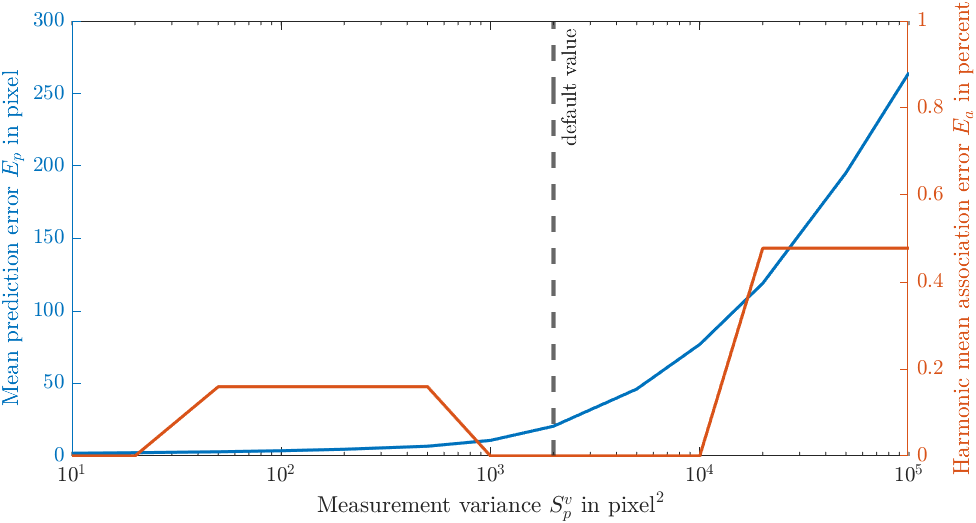
\includegraphics[width=0.9\textwidth]{figures/KF/meacov pfeffer cv2.png}
\caption{The grid search result of the measurement variance $S^{\boldmath{v}}$ of a peppercorn dataset with the CV model.}
\label{meacov}
\end{figure}

\begin{figure}[htbp]
\centering
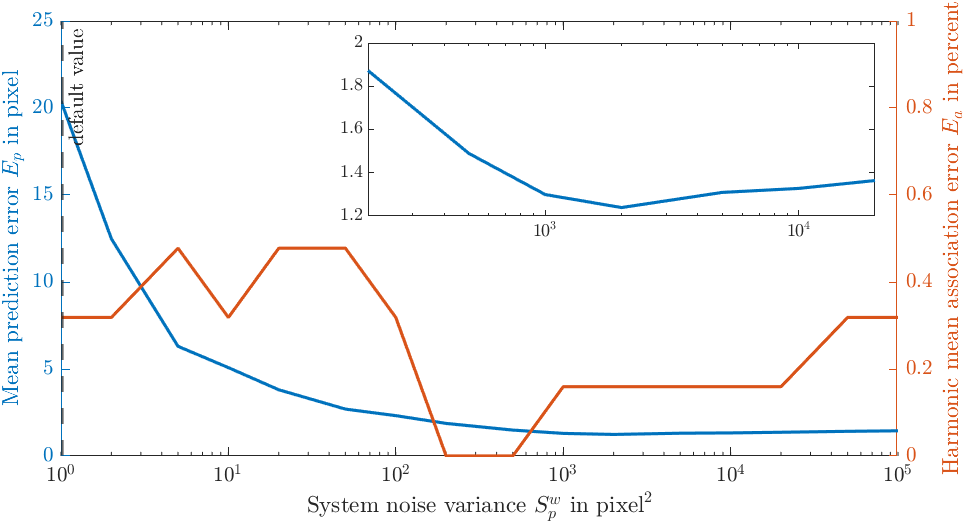
\includegraphics[width=0.9\textwidth]{figures/KF/precov pfeffer cv .png}
\caption{The grid search result of the system noise variance $S^{\boldmath{w}}$ of a peppercorn dataset with the CV model. The small plot shows that the $E_{\mathrm{p}}$ reaches minimum when the $S^{\boldmath{w}}$ is approximately 2,000.}
\label{precov}
\end{figure}

Figures \ref{meacov} and \ref{precov} show the grid search results of the measurement variance $S^{\boldmath{v}}$ and the system noise variance $S^{\boldmath{w}}$ in the CV model. As can be seen in Figure \ref{meacov}, the prediction error was lowered with a lower $S^{\boldmath{v}}$. Figure \ref{precov} shows that a higher $S^{\boldmath{w}}$ also leads to a lower prediction error. The minimized error in both figures is significantly lower than the error with the default hyperparameters. These results suggest a large potentiality for optimization. 

We can make an assumption based on these results. The predictions from the previous steps can be inaccurate because of the difference between the assigned velocity at initialization and the real velocity of the particle, or the difference between the motion model and the real motion of the particle. Thus, the prediction system should use a higher system noise variance to dismiss the error in the previous prediction and a lower measurement variance to keep up with the newest measurement. However, a very high system noise variance means the uncertainty of the previous prediction is very high, and the information contained with the previous prediction is in the update step fully ignored. In this case, the prediction error is heavily affected by the measurement error, which can also cause a higher total error, as shown in the subplot in Figure \ref{precov}. We can observe in that plot that when the system noise variance is about 2,000, the prediction error is minimized. According to the update equation in the Kalman filter, the ratio of the different variances determines the updated value. It means that increasing the $S^{\boldmath{v}}$ has a similar effect of decreasing the $S^{\boldmath{w}}$, when the effects of other hyperparameters are not remarkable. The result of grid search fits this theory well.

% However, when the measurement position error is too low, the change of the prediction error becomes ambiguous. The effects of the different hyperparameters are strongly related, where the final effect depends on the ratio of the hyperparameters. When some of the covariance or variance is too low, it means the certainty of the corresponding variable is very high, and the information contained with other variables is eliminated. In contrast, when some of the covariance or variance is too high, it means the uncertainty of the corresponding variable is very high, and the information contained with the variables is ignored. Therefore, when the hyperparameter is too low or too high, the effect on the prediction error is always not so significant. 

% \textcolor{red}{changed this para}
% With the default association hyperparameters, the association error is higher when the measurement variance is low. As mentioned, when the measurement variance is very low, the prediction error is increased because of the measurement error, which can cause a bad effect on the prediction and the association of the next timestep. However, with a higher $d_{\mathrm{am}}$, which increases the penalty of the new track appearing at middle, the association error is effectively suppressed. The association error stays below 0.5\% with the change of the system noise variance.  

\begin{figure}[htbp]
\centering
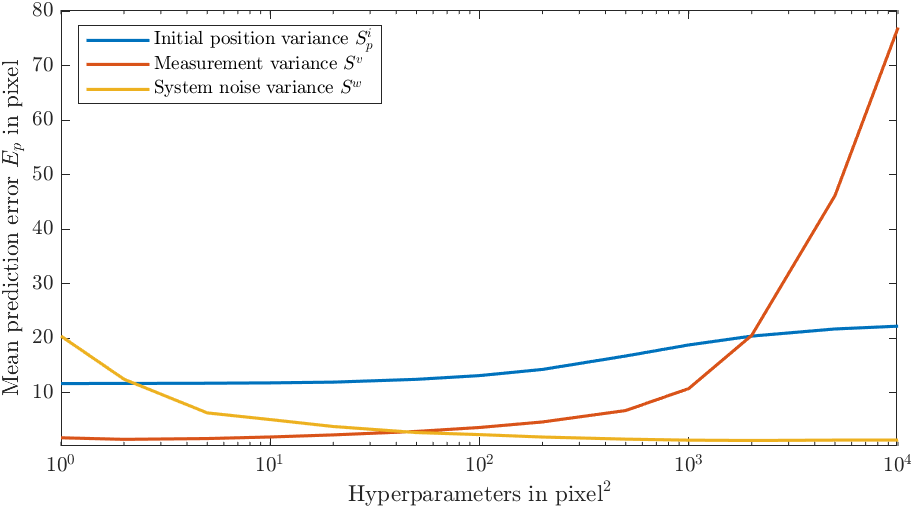
\includegraphics[width=0.8\textwidth]{figures/KF/3cov pfeffer cv.png}
\caption{The grid search result of $S^{i}_{p}$, $S^{\boldmath{v}}$ and $S^{\boldmath{w}}$ of a peppercorn dataset with the CV model.}
\label{3cov}
\end{figure}


Figure \ref{3cov} shows the effect of the initial position variance, measurement variance and system noise variance in the CV model. 
% \textcolor{red}{initial position noise variance, measurement noise variance and prediction noise variance, only the initial one has "position", because the velocity variance is different.}
For each line in this plot, only the mentioned variance is changed and all the other hyperparameters remain as default value. We can see that adjusting the measurement and the system noise variance has a clear effect on the prediction error. Although changing the value of the initial position variance has an effect on the prediction error as well, the effect is not as significant as the other two noise power spectral densities. 

\begin{figure}[htbp]
	\centering
	\begin{subfigure}[t]{0.8\textwidth}
		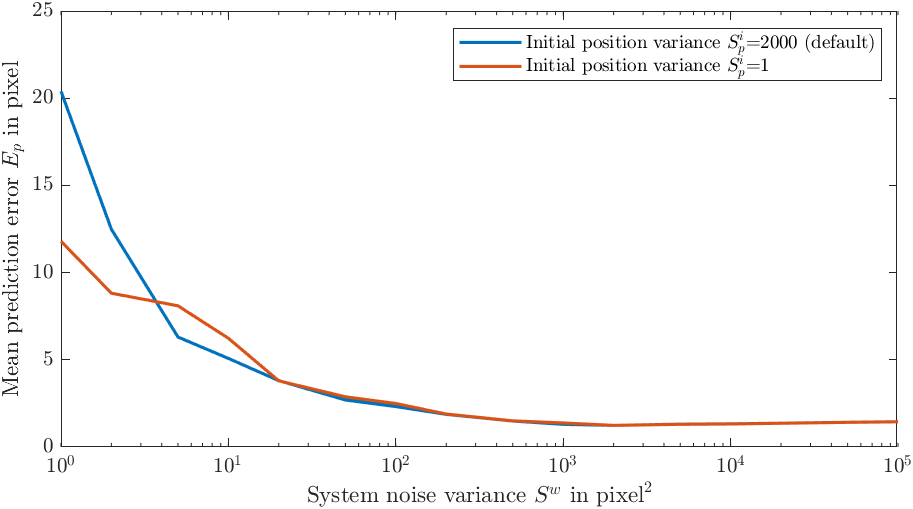
\includegraphics[width=\textwidth]{figures/KF/precov with inicov cv.png}
		\caption{The grid search result of the system noise variance in CV model with varied initial position variance.}
		\label{grid search different default1}
	\end{subfigure}
\end{figure}

\begin{figure}[htbp]
    \ContinuedFloat
    \centering
% 	\vskip\baselineskip
	\begin{subfigure}[t]{0.8\textwidth}
		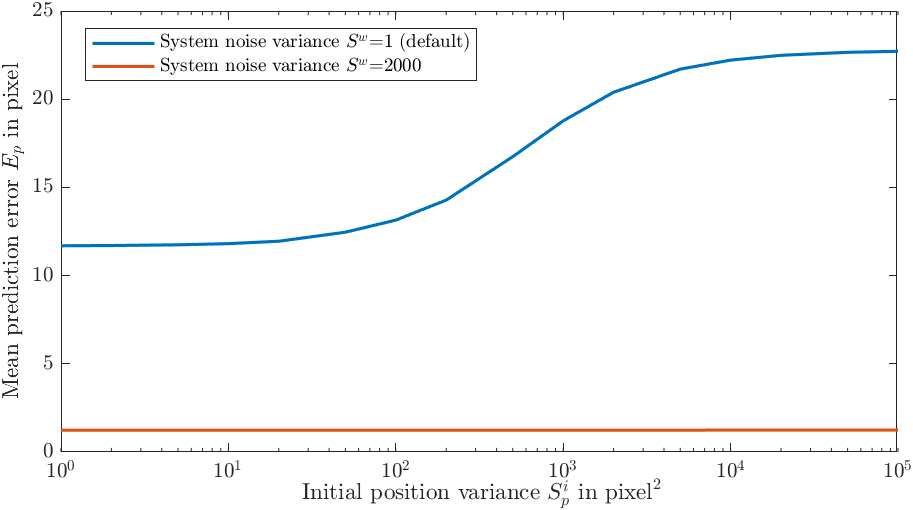
\includegraphics[width=\textwidth]{figures/KF/inicov with precov cv.png}
		\caption{The grid search result of the initial position variance in CV model with varied system noise variance.}
		\label{grid search different default2}
	\end{subfigure}
	\caption{The grid search results of initial position and system noise variance in CV model with only changing these two variance.}
	\label{grid search different default}
\end{figure} 
Figure \ref{grid search different default} presents the grid search results of the initial position and system noise variance in the CV model with varied other variance. In these figures, only the initial position and system noise variance are changed. When the initial position variance is higher, the trend of the prediction error with varied system noise power spectral densities only has a moderate change. But when the system noise variance reaches a high value, the initial position variance has no more effect on the prediction error. It means that the measurement and system noise variance are more valuable to optimize than the initial position variance. After checking the other hyperparameters, as shown in Figure \ref{grid search cv appendix} in Appendix, the measurement and the system noise variance still have the most significant effect on the prediction error in the CV model. Thus, these two hyperparameters are selected for the next step of the optimization.

The result of the CVA model is similar to the CV model. The optimized measurement position variance is lower than the default value, and the optimized prediction position variance is higher than the default. And these two hyperparameters are the most effective hyperparameter among all the hyperparameters for the prediction error. The result is shown in Figure \ref{grid search list} in Appendix. The dataset from each type of the homogeneous material was tested with grid search in both CV and CVA models. The effects of the hyperparameters are similar, which can be seen from Figure \ref{grid search other material} in Appendix. 
% From the the plots the effect of each hyperparameter is clear. We can also find the measurement and system noise variance have the most significant effect on the final tracking error. It should be a important result which is used in the part of optimization. 

\subsubsection{Result of 2-D Grid Search}

% \textcolor{red}{added new section}

Figure \ref{2d cv} shows the test result of a 2-D grid search with the measurement and system noise variance in the CV model. Same as the results from the 1-D grid search, the prediction error is lowered with a lower measurement variance and a higher system noise variance. We can also observe the dark blue area that means the prediction error is minimized. The shape of this area also suggests that the optimized value of the $S^{\boldsymbol{v}}$ and $S^{\boldsymbol{w}}$ should be proportional. The result of the 2-D grid search with the measurement and prediction position variance in the CVA model is illustrated in Figure \ref{2d cva}. A certain area for the optimized hyperparameters is unable to be observed from the plot, but the result still shows that the optimized value of two hyperparameters should be proportional.

\begin{figure}[htbp]
\centering
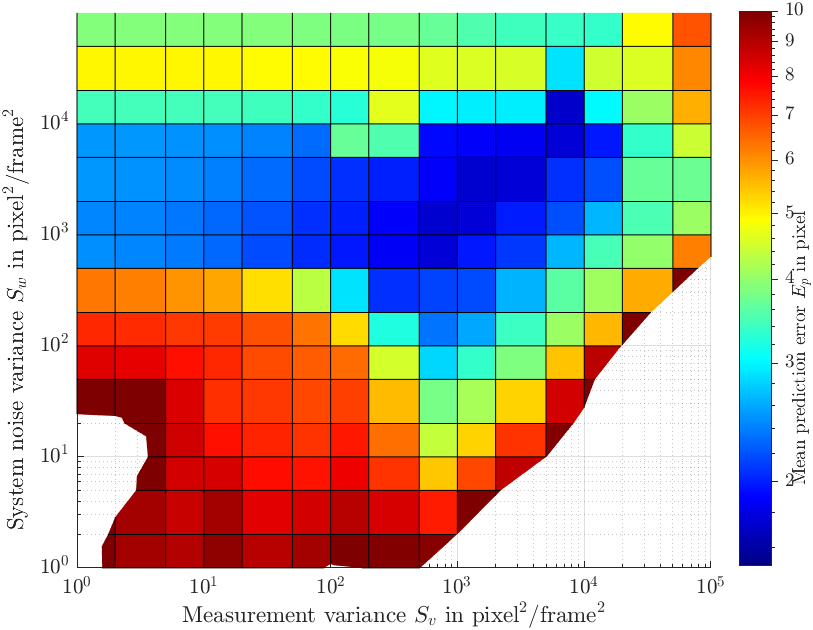
\includegraphics[width=0.8\textwidth]{figures/KF/2d cv1.png}
\caption{The 2-D grid search results of the measurement variance $S^{\boldsymbol{v}}$ and the system noise variance $S^{\boldsymbol{w}}$in the CV model. The data points with the $E_{\mathrm{p}}$ higher than 10 are not shown in this plot.}
\label{2d cv}
\end{figure}

\begin{figure}[htbp]
\centering
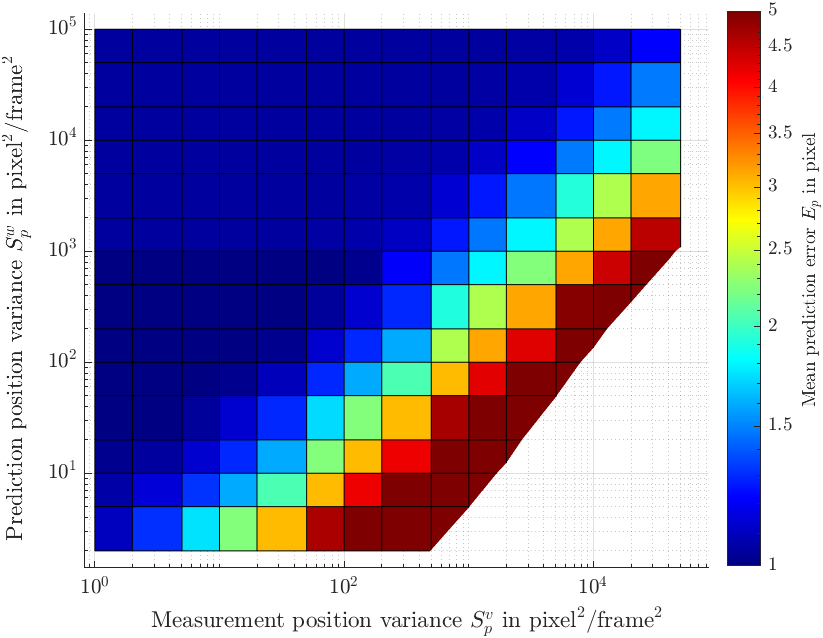
\includegraphics[width=0.8\textwidth]{figures/KF/2d cva1.png}
\caption{The 2-D grid search results of the measurement position variance $S_{\mathrm{pos}}^{\boldsymbol{v}}$ and the prediction position variance $S_{\mathrm{pos}}^{\boldsymbol{w}}$ in the CVA model. The data points with the $E_{\mathrm{p}}$ higher than 10 are not shown in this plot.}
\label{2d cva}
\end{figure}


% \subsubsection{Conclusion}

% From the results above, we can conclude that the prediction error is lower with 

% There should be the plots from 2-3 sets of hyperparameters in both CV and CVA model, e.g. measurement position covariance and initial position covariance. The main aim of this part is to show the different effect when two hyperparameter change at the same time. One hyperparameter should have more effect than the other one, so we can find the difference of the "important" and "unimportant" hyperparameters raised in the last section.

% \FloatBarrier

% \subsection{Results of Bayesian Optimization}

\subsection{Validation of the Bayesian Optimization Method}
\label{validation}
% Give some introduction of generating datasets. 
% Add a table of some experiment results of the generated datasets. The results from the optimization is very similar from the real parameters, showing the optimization method can reconstruct the real hyperparameters of the system.

In order to confirm the validity of the Bayesian optimization method, the implemented optimization algorithm was first tested with artificial datasets. During the optimization, only one or two hyperparameters were optimized at the same time, and the other hyperparameters kept the same value with the setting for generating the dataset. When the optimized values of the hyperparameters are the same as the value in the setting, the optimization algorithm can be recognized to be able to reconstruct the hyperparameters in the system.

% To overcome the interference of the random noise, the optimization for each hyperparameter was done with ten datasets under the same settings, as mentioned in \Sec{Artificial Datasets}. The final optimization result is the average value of the optimized result from all datasets.

The result of the optimized hyperparameters and the original hyperparameters from the dataset are presented in Table \ref{validationHPs} and \ref{validationHPs2d}. The difference between the value of the hyperparameters given in the dataset generation and the value of the optimized hyperparameters is lower than 1\% on average. These results suggest that the Bayesian optimization method can reconstruct the real hyperparameters of the system. 

\begin{table}[htbp] 
    % \small
    \centering
    \caption{Optimized hyperparameters and the original hyperparameters from the dataset in the validation dataset in 1-D Bayesian optimization. The original and optimized values are similar, which suggests that the Bayesian optimization method is able to reconstruct the hyperparameters in a dynamic system.} 
    \begin{tabular}{cccc} 
    \toprule 
    \multirow{2}*{Model}&\multirow{2}*{Hyperparameters}&Original &Optimized \\ 
         &               &value&value\\ 
    \midrule 
    \multirow{3}*{CV}&Measurement variance  $S^{\boldsymbol{v}}$&0.1&0.10020\\
     &System noise variance $S^{\boldsymbol{w}}$&0.1&0.10045\\
     &Initial velocity $v_{0}$&100&100.01\\
    \multirow{4}*{CVA}&Measurement position variance $S_{\mathrm{pos}}^{\boldsymbol{v}}$  &0.1&0.10081\\
     &Prediction position variance $S_{\mathrm{pos}}^{\boldsymbol{w}}$&0.1&0.09820\\ 
     &Measurement velocity variance $S_{\mathrm{vel}}^{\boldsymbol{v}}$&0.1&0.09923\\ 
     &Initial velocity $v_{0}$&100&100.02\\
    \bottomrule 
    \end{tabular} 
    \label{validationHPs}
\end{table}

\begin{table}[htbp] 
    % \small
    \centering
    \caption{Optimized hyperparameters and the original hyperparameters from the dataset in the validation dataset in 2-D Bayesian optimization. The original and optimized values are similar, which suggests that the Bayesian optimization method is able to reconstruct the hyperparameters in a dynamic system.} 
    \begin{tabular}{cccc} 
    \toprule 
    \multirow{2}*{Model}&\multirow{2}*{Hyperparameters}&Original &Optimized \\ 
         &               &value&value\\ 
    \midrule 
    \multirow{2}*{CV}&Measurement variance  $S^{\boldsymbol{v}}$&0.1&0.10071\\
     &System noise variance $S^{\boldsymbol{w}}$&0.1&0.09898\\
    \multirow{2}*{CVA}&Measurement position variance $S_{\mathrm{pos}}^{\boldsymbol{v}}$  &0.1&0.10145\\
     &Prediction position variance $S_{\mathrm{pos}}^{\boldsymbol{w}}$&0.1&0.09912\\
    \bottomrule 
    \end{tabular} 
    \label{validationHPs2d}
\end{table}



However, we only tested the case, where the motion of the particles follows exactly the motion model. The effect of the difference between the real motion and the motion models on the hyperparameter is not examined. These effects are hard to express with the functions of the hyperparameters. Therefore, we are unable to check this effect with the artificial data with the method in this section.

\subsection{Results of Bayesian Optimization on the Peppercorn Dataset}
\label{Tests of Bayesian Optimization}
\subsubsection{Results of Bayesian Optimization in Higher Dimension}

In \Sec{1d}, the most effective hyperparameters for both motion models were given. In this section, these hyperparameters were optimized with the Bayesian optimization algorithm. According to the update equation in the Kalman filter, the ratio of the different variances determines the updated value. The 2-D optimization result presented in Figure \ref{opt 2d} also shows that the optimized values of the two hyperparameters are proportional. This feature enables us to operate the optimization with only one hyperparameter. Thus, the search space for optimization is reduced, which can increase the accuracy and efficiency of the optimization.
% \textcolor{red}{the algorithm converges faster when optimizing only 1 HP.} 

\begin{figure}[htbp]
\centering
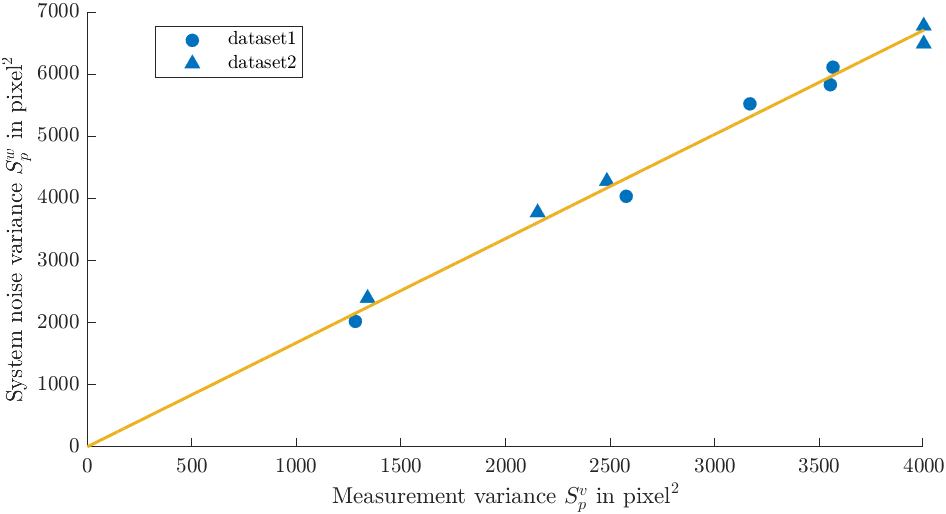
\includegraphics[width=0.7\textwidth]{figures/KF/bayopt/opt 2d cv.png}
\caption{The result of the 2-D optimization of $S^{\boldsymbol{v}}$ and $S^{\boldsymbol{w}}$ with two peppercorn datasets. The optimized values of the two hyperparameters are proportional.}
\label{opt 2d}
\end{figure}

\begin{figure}[htbp]
\centering
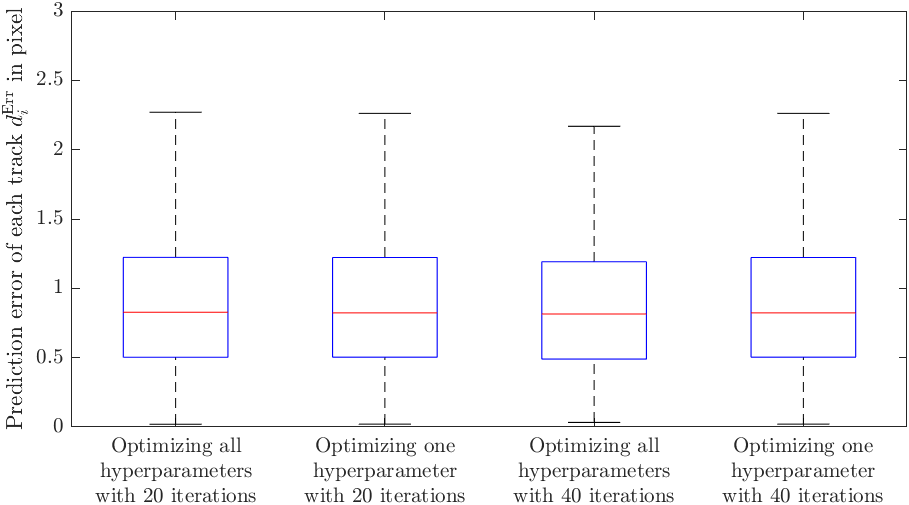
\includegraphics[width=0.7\textwidth]{figures/KF/bayopt/effect opt all.png}
\caption{The comparison of the 5-D optimization result of all hyperparameters in CV model and the 1-D optimization result of $S^{\boldsymbol{w}}$ with a peppercorn datasets. }
\label{opt 5d}
\end{figure}

Figure \ref{opt 5d} shows the comparison of the 5-D optimization result of all hyperparameters in the CV model and the 1-D optimization result of $S^{\boldsymbol{w}}$ with a peppercorn dataset. We can observe that the prediction error from the 1-D optimization is very similar to the prediction error from the 5-D optimization. And the difference from the prediction error with different iterations is also not significant. Therefore, using the 1-D Bayesian optimization with 20 iterations is enough to obtain satisfactory results on the optimized hyperparameters. Based on these results, we can confirm that the 1-D Bayesian optimization can archive a similar effect as the optimization with higher dimensions. Therefore, in the following sections we are using the 1-D Bayesian optimization.   



% We find first that when we optimizing two hyperparameters at the same time, the two optimized hyperparameters are proportional. It shows that the effect of the other HPs are less. That also enables us to operate the optimization with only one HP, which can increase the accuracy and the efficiency of the optimization.

% Some optimization results with different models (CV and CVA) and different datasets (sphere, cylinder, cuboid and pepper).

\subsubsection{Results of 1-D Bayesian Optimization}

In the following sections, only the system noise variance $S^{\boldsymbol{w}}$ in the CV model and the prediction position noise power spectral density $S_{\mathrm{pos}}^{\boldsymbol{w}}$ in the CVA model is optimized, and the other hyperparameters remain the default values. Figure \ref{opt cv sph} shows an intermediate result of the Bayesian optimization of a sphere dataset with the CV model. The algorithm constructs a surrogate model for the prediction error.

\begin{figure}[htbp]
\centering
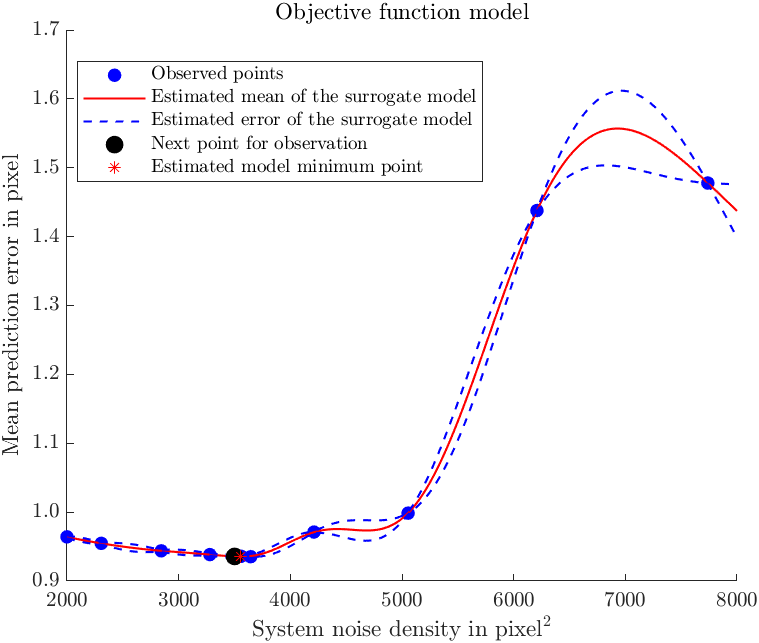
\includegraphics[width=0.6\textwidth]{figures/KF/bayopt/bayopt line pfeffer.png}
\caption{The intermediate result of the Bayesian optimization of a peppercorn dataset with the CV model.}
\label{opt cv sph}
\end{figure}

In Figures \ref{opt effect1} and \ref{opt effect2} the effect of the optimization is visualized with box plots. The plots present the distribution of the prediction errors of all tracks in the peppercorn dataset for test. The upper and lower bound of the boxes in the box indicate respectively the upper quartile $Q_{3}$ and lower quartile $Q_{1}$ of the errors, and the red line in the middle of boxes represents the median of the errors. The maximum length of the whiskers is determined as $1.5(Q_{3}-Q_{1})$. The outliers are not shown in the plots.


From the box plots, we can observe that the accuracy of the prediction with optimized hyperparameters is significantly higher than with the default hyperparameters. The prediction error with optimized hyperparameters is also approximately 10\% lower than the results from Hornberger \cite{hornberger2018} in the CV model. The association error with the optimized hyperparameters is limited in an acceptable range, which is less than 1\% in each dataset.

In Table \ref{opt pfeffer}, the optimized values of the hyperparameters from grid search have a significant difference from the results from Bayesian optimization because of high step size. The results with the hyperparameters from Bayesian optimization are also slightly better than the results from grid search. Because of the settings of the grid points, grid search is not always able to find the optimized value for the hyperparameters. Although employing a smaller step size can increase the possibility of finding the optimized value, the computation need is also increasing. In this respect, Bayesian optimization is a more efficient method for hyperparameter optimization.





\begin{table}[htbp] 
\small
    \centering
    \caption{List of the default and optimized value of the $S^{\boldsymbol{w}}$ in the CV model and $S_{\mathrm{pos}}^{\boldsymbol{w}}$ in the CVA model for the peppercorn dataset.} 
    \begin{tabular}{ccc} 
    \toprule 
    Hyperparameters &Optimization method  &Value\\ 
    \midrule 
    \multirow{3}*{$S^{\boldsymbol{w}}$}&  Default   &1\\
    &Optimized with grid search                     &2000\\
    &Optimized with Bayesian optimization           &3508.1\\
    \multirow{3}*{$S_{\mathrm{pos}}^{\boldsymbol{w}}$}&Default &16.7\\
    &Optimized with grid search                     &20000\\
    &Optimized with Bayesian optimization           &20301\\
    \bottomrule 
    \end{tabular} 
    \label{opt pfeffer}
\end{table}

\begin{figure}[htbp]
\centering
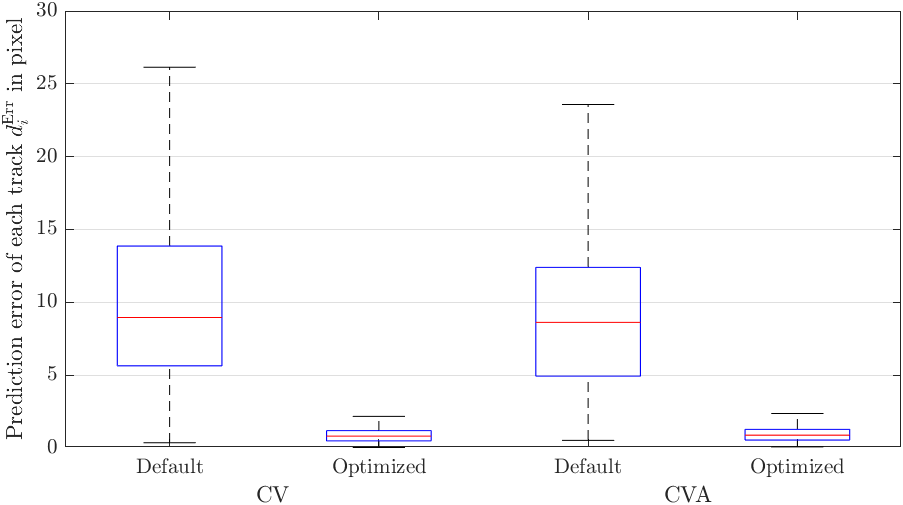
\includegraphics[width=0.7\textwidth]{figures/KF/bayopt/effect opt4.png}
\caption{Comparison of the prediction error with the default and optimized hyperparameters with the peppercorn datasets.}
\label{opt effect1}
\end{figure}

\begin{figure}[htbp]
\centering
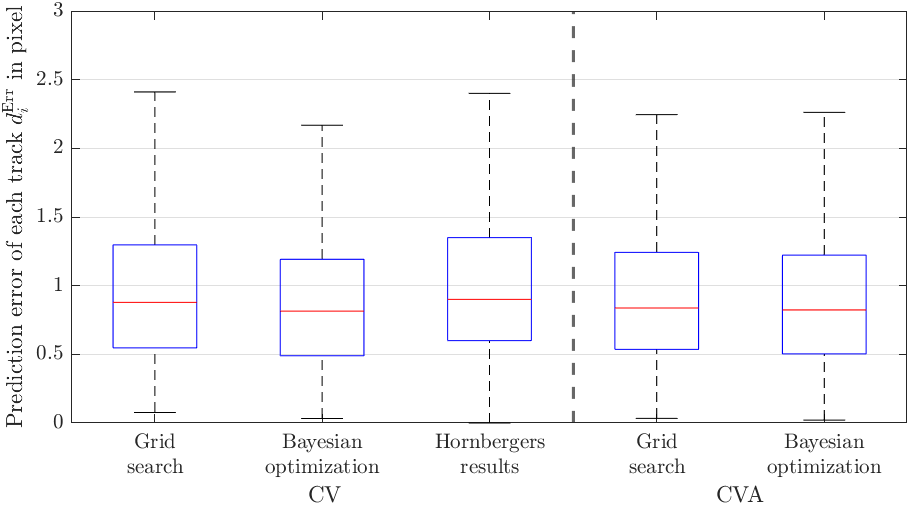
\includegraphics[width=0.8\textwidth]{figures/KF/bayopt/effect opt3.png}
\caption{Comparison of the prediction error with the hyperparameters from different optimization methods with the peppercorn datasets.}
\label{opt effect2}
\end{figure}

% \subsection{Clustering and Mapping}
\subsection{Results of Bayesian Optimization with Different Materials}
\label{Test of Different Materials}
\subsubsection{Results of Homogeneous Materials}
% Try to make clusters between different datasets. Make plots showing results from different datasets. The results from different datasets are similar within the same datasets and different between different datasets, showing the different materials applies for different hyperparameters. After that give some analysis or assumption of the reason causing these difference between the datasets. 

Figures \ref{cluster1} and \ref{cluster2} present the optimized values of the system noise variance in the CV model and the system position noise power spectral density in the CVA model for varied materials.
% \textcolor{red}{You highlighted here. Is that too long?} 
It can be seen from the optimization result that different materials have different ranges of optimized hyperparameters. The comparison of the prediction error between different optimization methods of each material is presented in Figure \ref{effect opt appendix} in Appendix.

The difference between the optimized hyperparameters comes primarily from the difference in the motion characteristics of the different types of materials. For example, the spheres are easy to roll on the conveyor belt, but the cylinders can roll only when the particle lies in a specific direction. That means the velocities of spheres are more likely to be different from the belt velocity than cylinders. These characteristics make the real motion of the particles different from the motion model, and this difference needs to be compensated from the noise term in the motion model. Therefore, the different values of the hyperparameters that represent the different system and measurement noise power spectral densities should be applied to different types of materials.

\begin{figure}[htb]
\centering
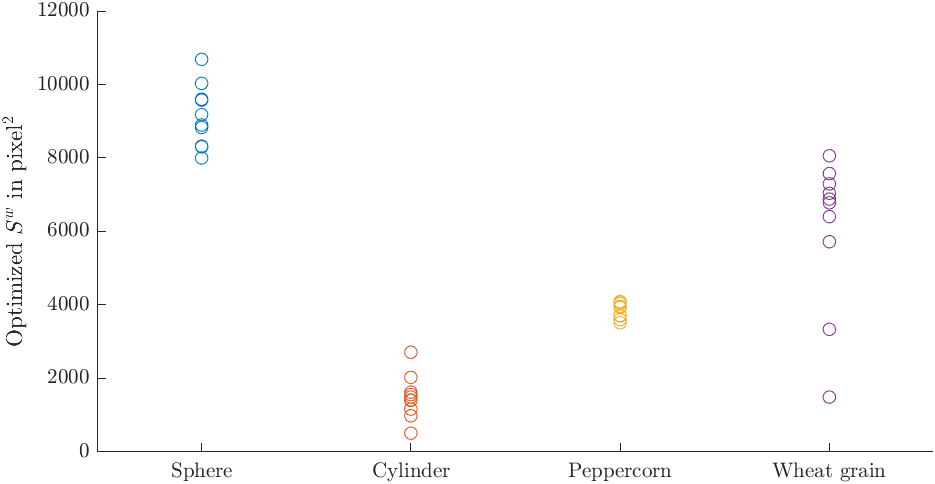
\includegraphics[width=0.7\textwidth]{figures/KF/bayopt/opt all CV.png}
\caption{The optimized value of the system noise variance in CV model for different materials.}
\label{cluster1}
\end{figure}

\begin{figure}[htb]
\centering
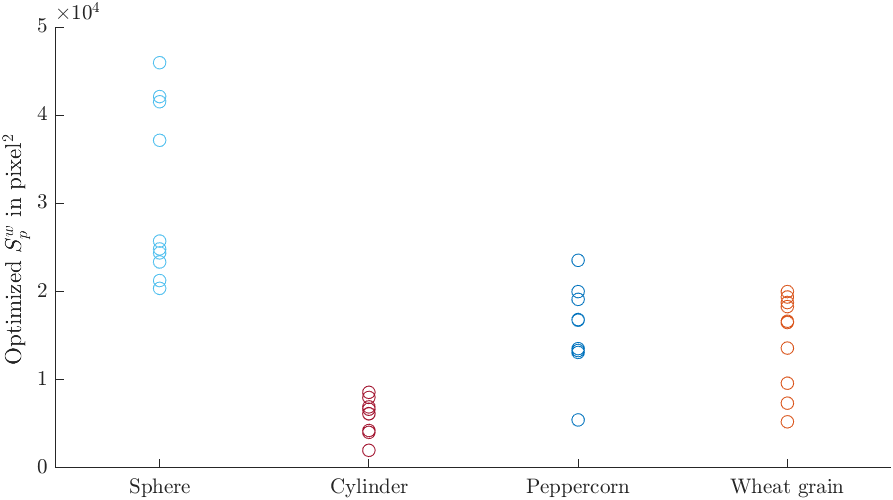
\includegraphics[width=0.7\textwidth]{figures/KF/bayopt/opt all CVA.png}
\caption{The optimized value of the system position noise power spectral density in CVA model for different materials.}
\label{cluster2}
\end{figure}

However, the optimized values of the hyperparameters are distributed in a wide range, and the range of the hyperparameters of various materials often overlaps from each other. For example, the range for the peppercorn and the wheat grain is very similar in Figure \ref{cluster2}. It makes the clustering work more challenging. This phenomenon is possibly due to the ``flat area" in the hyperparameter space. As shown in Figure \ref{precov}, the error in a wide range around the optimal value of the hyperparameter remains almost the same. It means a slight random error in the tracking process can cause a remarkable difference in the optimization result. The wide distribution of the optimized hyperparameters can also attribute to some other differences between datasets, such as the density of the particles on the belt.


\FloatBarrier

\subsubsection{Results of Mixed Materials}


Table \ref{resultmix} presents the result of the optimized value of the $S^{\boldsymbol{w}}$ and $S_{\mathrm{pos}}^{\boldsymbol{w}}$ for the mixture materials dataset. We observed that the optimized $S^{\boldsymbol{w}}$ and $S_{\mathrm{pos}}^{\boldsymbol{w}}$ here is much lower than the value from the homogeneous materials. 

The shape and size features can have an effect on the measurement noise. The particle size in the mixture varies dramatically, while the size of homogeneous materials is the same within a dataset. The shapes of the mixture materials are also irregular. These characteristics increase the hurdles of detecting the midpoint location of the particles, which also increases the measurement noise. Because of the high noise, the track results are heavily affected by the random factors, which causes the optimized hyperparameters in different datasets distributed in a wide range. The comparison of the prediction errors with the default and optimized hyperparameters with the mixed material datasets.

\begin{table}[htbp] 
\centering
\caption{List of the optimized value of the $S^{\boldsymbol{w}}$ and $S_{\mathrm{pos}}^{\boldsymbol{w}}$ for the mixture materials dataset.} \small
\begin{tabular}{ccc} 
\toprule 
Hyperparameters &Dataset &Value\\ 
\midrule 
\multirow{3}*{$S^{\boldsymbol{w}}$}& 1 &9609.8\\
&2 &2350.1\\
&3 &570.6\\
\multirow{3}*{$S_{\mathrm{pos}}^{\boldsymbol{w}}$}&1 &15227.3\\
&2 &2104.8\\
&3 &4136.3\\
\bottomrule 
\end{tabular} 
\label{resultmix}
\end{table}

\FloatBarrier

\section{Robust Range of Association Hyperparameters}
\label{Robust Range of Association Hyperparameters}

\subsection{Results with Grid Search}

\begin{figure}[htb]
\centering
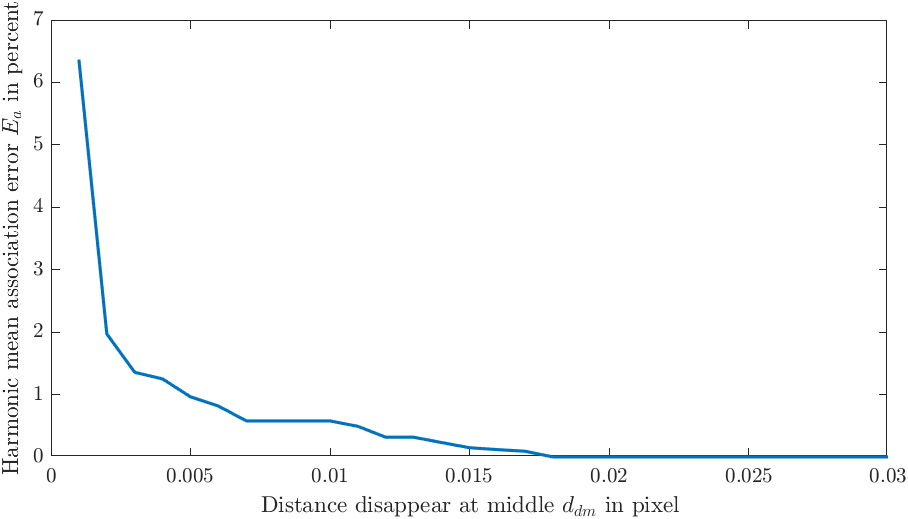
\includegraphics[width=0.8\textwidth]{figures/Asso/gridsearch1.png}
\caption{The grid search result of the distance disappear at middle $d_{\mathrm{dm}}$ on the association error with the DEM dataset.}
\label{asso gs1}
\end{figure}

\begin{figure}[htb]
\centering
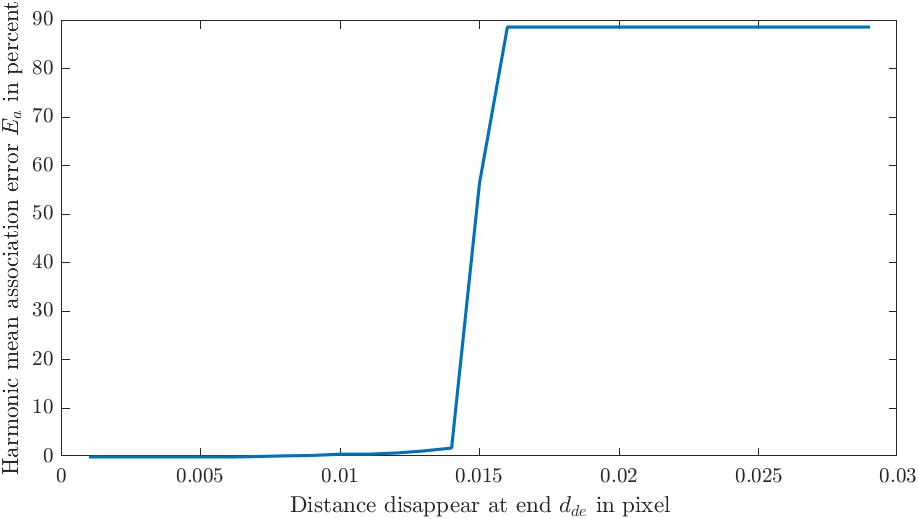
\includegraphics[width=0.8\textwidth]{figures/Asso/gridsearch2.png}
\caption{The grid search result of the distance disappear at end $d_{\mathrm{de}}$ on the association error with the DEM dataset.}
\label{asso gs2}
\end{figure}

The effects of the association hyperparameters are first tested with grid search on the DEM dataset. Figures \ref{asso gs1} and \ref{asso gs2} reveal the effect of the distance disappear at middle $d_{\mathrm{dm}}$ and the distance disappear at end $d_{\mathrm{de}}$ on the association error. According to Figure \ref{asso gs1}, the tracking results have no association error as the $d_{\mathrm{dm}}$ is higher than 0.018. Therefore, the range above 0.018 can be considered as the robust range for $d_{\mathrm{dm}}$. However, when the distance decreases lower than 0.018, the association error begins to increase slightly. When the distance is more close to zero, the association error increases more sharply. The distance disappear at end has a robust range below 0.005, as shown in Figure \ref{asso gs2}. The association error grows steadily with the increase of the distance lower than 0.014, and then have a steep increase between 0.014 and 0.016. After that, the association error reaches nearly 90\%, which indicates the tracking algorithm is unable to provide a reasonable association in this range. These results are easy to understand qualitatively: a particle is less possible to leave the tracking area at the middle of the area, but more possible to leave at the end phase. Therefore, the distance disappear at middle should be higher, and the distance disappear at end should be generally low. The effect of the other hyperparameters is also examined with the same method, and the results are presented in Figure \ref{grid search other} in Appendix.

% Similar to the part of the prediction hyperparameters, each association  hyperparameter is also tested with the grid-search-like method, in order to find the effect of each hyperparameter on the association error.

% ...The distance ...should be higher....and ... should be lower....


% \FloatBarrier


\subsection{Results with SVM}

% (Results with SVM)
% Several plots like this. After plots give some analyze ().

After the grid search, some SVMs were trained with the training dataset mentioned in \Sec{training data svm}. The SVMs present the range of the association hyperparameters with no association hyperparameters. This range can represent the robust range of the association hyperparameters.

Some results of the robust range acquired from two-dimensional SVMs are depicted in Figures \ref{svm1} and \ref{svm2}. In Figure \ref{svm1} we can observe that the robust range of the distance disappear at middle $d_{\mathrm{dm}}$ is roughly above 0.018, which meets the result from the grid search. The lower bound of the distance appear at middle $d_{\mathrm{am}}$ is unable to see from the plot. We can make an assumption that the lower bound of the distance appear at middle could be lower than zero. However, we can still notice that when the $d_{\mathrm{dm}}$ is close to zero, the lower bound for the robust range of the $d_{\mathrm{am}}$ increases to 0.02. It means there is still a correlation between the value and the robust range of the two hyperparameters.

\begin{figure}[htb]
\centering
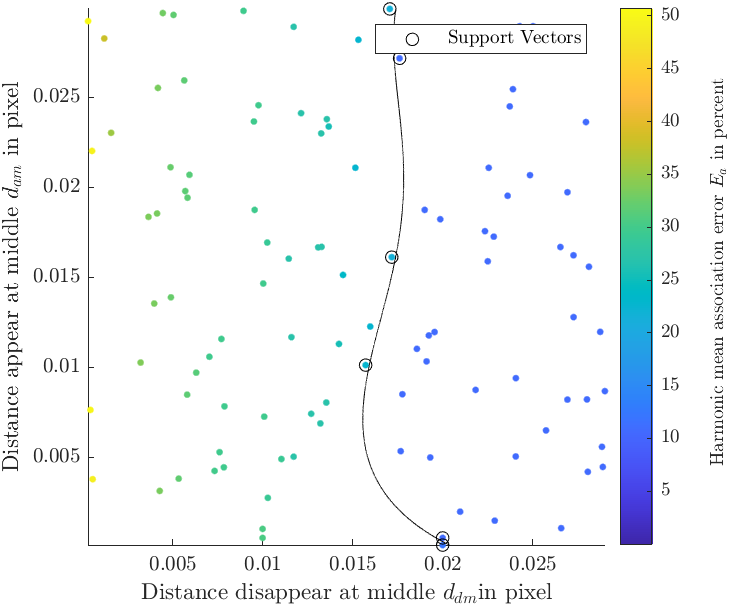
\includegraphics[width=0.6\textwidth]{figures/Asso/overfitting2.png}
\caption{The 2-D SVM result of the distance disappear at middle and the distance appear at middle with DEM dataset.}
\label{svm1}
\end{figure}

Figure \ref{svm2} shows the robust range of the distance disappear at middle and the distance no change. It is obvious that the lower bound for the distance disappear at middle $d_{\mathrm{dm}}$ is strongly related to the value of the distance no change $d_{\mathrm{n}}$. Recalling the example raised in \Sec{Robust Range of the Association Hyperparameters}, the results shown in two figures conform to the theoretical analysis of the robust range. When the distance no change is higher, the sum of the distance disappear at middle and the distance appear at middle should be also higher for a correct association.

\begin{figure}[htb]
\centering
\includegraphics[width=0.6\textwidth]{figures/Asso/2d svm.png}
\caption{The 2-D SVM result of the distance no change and the distance appear at middle with DEM dataset.}
\label{svm2}
\end{figure}

\begin{figure}[htb]
\centering
\includegraphics[width=0.5\textwidth,height=0.5\textwidth]{figures/Asso/2d svm sphere.png}
\caption{The two dimensional SVM result of the distance disappear at middle and the distance appear at middle with the sphere dataset.}
\label{svm3}
\end{figure}

However, the robust range of association hyperparameters for different datasets can be very different. In Figure \ref{svm3}, the lower bound for the distance appear at middle $d_{\mathrm{am}}$ for the sphere dataset is about two. Since the tracking error of the different datasets is different, the association hyperparameters should be certainly different. Therefore, the robust range of association hyperparameters for different datasets should be determined separately. However, the datasets that have similar tracking errors are acceptable to take the same robust range of association hyperparameters. For example, all the experiments on the hyperparameters for motion prediction with real datasets are performed with the same association hyperparameters.


The shape of the boundary curve of the robust range for the sphere dataset is similar to the DEM dataset. It suggests that the reasons for those curve shape for different materials are also similar. These reasons are explained in the next section.

In order to determine the robust range in a higher-dimensional space, the SVMs were also trained with varying all the five association hyperparameters. To examine the accuracy of the trained SVMs, the SVM classifiers were tested with the test dataset. The test result is shown in Table \ref{svm test}. It shows that the SVM classifiers have obtained a satisfactory classification accuracy. The decision boundary in the 3-D space is shown in Figure \ref{3d svm}.


\begin{table}[htb] 
    \centering
    \caption{Classification accuracy of the SVM classifiers on the test dataset.} 
    \begin{tabular}{ccc} 
    \toprule 
     & Classified as & Classified as\\ 
     & with association errors & no association errors\\
    \midrule 
    with association errors & 500 &14 \\
    no association errors   & 3  &483 \\
    \bottomrule 
    \end{tabular} 
    \label{svm test}
\end{table}



\begin{figure}[htbp]
\centering
\includegraphics[width=0.7\textwidth]{figures/Asso/3d svm.png}
\caption{The decision boundary of the SVM in 3-D space.}
\label{3d svm}
\end{figure}


\FloatBarrier

\subsection{Analysis of the Robust Range of the Association Hyperparameters}

% \textcolor{red}{write something about the effect of the hyperparameters. How it controls the association. Why some should low and why should some high}

Considering only the association error caused by inappropriate association hyperparameters, the error can be divided into two types, as illustrated in Figure \ref{association error example}. The first type is that a single track is separated into two tracks in the middle. When the distance no change is too high or the other distance is too low, this error happens. Take the association matrix in Figure \ref{asso example simple} as an example, when the summation of the distance between the prediction and the new measurements, as the left above block, and the distance no change is higher than the summation of the other two distances, the GNN algorithm would choose the left below and the right above blocks, which means there is a track with no assigned measurements and a new track. To avoid this error, the distance no change should have an upper bound, and the other distances should have a lower bound. The upper and lower bound here are strongly related. This result can also explain the reason for the boundary shape of the robust ranges shown in Figures \ref{svm1}, \ref{svm2} and \ref{svm3}.

\begin{figure}[htbp]
\centering
\includegraphics[width=0.6\textwidth]{figures/Asso/association matrix example simple.png}
\caption{A simple example of the association matrix.}
\label{asso example simple}
\end{figure}

We take the maximum Mahalanobis prediction error $d_{\mathrm{pre-mea}}^{\mathrm{max}}$ representing the maximum Mahalanobis distance between associated predictions and measurements. In order to avoid the type of error mentioned above, we propose that the summation of the distance for appearing and disappearing should be lower than the summation of the $d_{\mathrm{pre-mea}}^{\mathrm{max}}$ and the distance no change $d_{\mathrm{n}}$. Therefore, the value of the hyperparameters follows these inequalities
\begin{equation}\label{assoeq1}
    d_{\mathrm{n}} + d_{\mathrm{pre-mea}}^{\mathrm{max}} \leqslant 
    \left\{
         \begin{array}{ll}
         d_{\mathrm{as}} + d_{\mathrm{dm}}, \quad&\textrm{for start phase}\\
         d_{\mathrm{am}} + d_{\mathrm{dm}}, \quad&\textrm{for middle phase}\\
         d_{\mathrm{am}} + d_{\mathrm{de}}, \quad&\textrm{for end phase}  
         \end{array}
    \right . 
\end{equation}

After manual checks, all the default values of the association hyperparameter for both real and DEM datasets are in the robust range. The $d_{\mathrm{pre-mea}}^{\mathrm{max}}$ in the DEM dataset with default hyperparameters is about $0.05$ m. The $d_{\mathrm{pre-mea}}^{\mathrm{max}}$ in the peppercorn dataset is about $0.35$ pixel with the default prediction hyperparameter. Therefore, the default hyperparameters fit in  Inequality \eqref{assoeq1}. A lower measurement covariance can increase the Mahalanobis distance. Because of this effect, the $d_{\mathrm{am}}$ is set higher as the default value when the measurement noise power spectral density is set at a low value.
% \textcolor{red}{since the default value is robust, I'm not going to do more other tests on the real datasets.}

\begin{figure}[htbp]
	\centering
	\begin{subfigure}[t]{0.3\textwidth}
		\includegraphics[width=\textwidth]{figures/Asso/association error example1.png}
		\caption{An association error occurred because a single track is separated into two tracks in the middle of the track.}
	\end{subfigure}
	\quad
	\begin{subfigure}[t]{0.3\textwidth}
		\includegraphics[width=\textwidth]{figures/Asso/association error example2.png}
		\caption{An association error occurred because a track can not end properly.}
	\end{subfigure}
	\caption{Two types of association errors caused by inappropriate association hyperparameters.}
	\label{association error example}
\end{figure}



Another type is that a track can not end properly. It means this track is not considered as ended when it reaches the end but assigned with a new appeared measurement. When the track disappears in the middle of the observation area, this type of error does not affect the final separation accuracy, since the number of tracks reaching the end of the observation area remains unchanged. However, when the track disappears in the end, this type of error will produce some tracks that contain only one or two measurements, which usually have a high prediction error. This type often happens when the distance disappear at end and the distance appear at start is too high, such as the area over 0.015 in Figure \ref{asso gs2}, because the tracks are mainly appearing at the start phase and disappearing in the end phase. However, when the datasets contain the tracks that should appear and disappear in the middle, the corresponding hyperparameters should have also a limited upper bound.

The distance between measurements and the other the predictions from other tracks $d_{\mathrm{other}}$ are introduced for explaining this type of error. Considering only the track reaches the end phase when the track is associated with a measurement not belonging to other tracks, the inequalities are presented as 
\begin{equation}
    \label{assoeq2}
    d_{\mathrm{other}} + d_{\mathrm{n}}\geqslant\  
    \left \{
    \begin{array}{ll}
    d_{\mathrm{am}} + d_{\mathrm{de}} ,\quad&\textrm{for the measurement in start phase}\\ 
    d_{\mathrm{as}} + d_{\mathrm{de}} ,\quad&\textrm{for the measurement in middle or end phase}
    \end{array}.  
    \right.  
\end{equation}
And when the associated measurement belongs to another existing track $i$, the inequalition is presented as
\begin{equation}
    d_{\mathrm{de}} + d_{i}^{\mathrm{Err}} \leqslant\  d_{\mathrm{other}} + d_{\mathrm{n}}.
    \label{assoeq3}
\end{equation}
These inequalities determine the upper bound of the $d_{\mathrm{de}}$, $d_{\mathrm{am}}$ and $d_{\mathrm{as}}$. The $d_{\mathrm{other}}$ is determined by the local density of the particles. Therefore, even if the overall density is low, the $d_{other}$ can be in some position high. However, the $d_{other}$ is determined by the overall density of particles on the belt in general.

From the analysis above, the robust range is greatly influenced by the average prediction error. Therefore, the quality of the motion prediction also causes a massive effect on the robust range of the association hyperparameters. When the prediction is more accurate, the association hyperparameters can allow a wider robust range without increasing the association error.

Theoretically, all the association hyperparameters should have a lower bound and an upper bound. However, in our search, there are some hyperparameters having a lower bound below than zero. A negative distance is out of the domain of definition. Therefore, the lower bound for the robust range is defined as zero in this case.


\begin{table}[htbp] 
    % \small
    \centering
    \caption{Two test sets of the robust and unrobust association hyperparameters for the peppercorn dataset.} 
    \begin{tabular}{ccc} 
    \toprule 
    Settings&Hyperparameters& Value\\ 
    \midrule 
    \multirow{5}*{Robust}&Distance appear at start $d_{\mathrm{as}}$&0.1\\
    &Distance appear at middle $d_{\mathrm{am}}$&0.18\\
    &Distance disappear at end $d_{\mathrm{de}}$&0.1\\
    &Distance disappear at middle $d_{\mathrm{dm}}$&0.18\\
    &Distance no change $d_{\mathrm{n}}$&0\\
    ~\\
    \multirow{5}*{Unrobust}&Distance appear at start $d_{\mathrm{as}}$&0.1\\
    &Distance appear at middle $d_{\mathrm{am}}$&0.15\\
    &Distance disappear at end $d_{\mathrm{de}}$&0.1\\
    &Distance disappear at middle $d_{\mathrm{dm}}$&0.15\\
    &Distance no change $d_{\mathrm{n}}$&0\\
    \bottomrule 
    \end{tabular} 
    \label{test robust}
\end{table}

With the analysis above, a set of robust association hyperparameters can also be determined for the dataset from real materials. From the results from the part of prediction hyperparameters, the average prediction error and the density of particles are similar in the peppercorn, sphere and wheat grain datasets with the optimized prediction hyperparameters. Therefore, these datasets can share the same values of hyperparameters. According to the average prediction error and the density of particles of the datasets, a set of the robust association hyperparameters is calculated with the Inequality \eqref{assoeq2} and \eqref{assoeq3}, as listed in Table \ref{test robust}. In the test of the association hyperparameters, the prediction hyperparameters take the optimized value from \Sec{opt pred}, and the test is operated under the CV model. The result of the association error with the three datasets presented in Table \ref{result robust} shows that the calculated robust hyperparameters stay indeed in the robust range.

\begin{table}[htbp] 
    % \small
    \centering
    \caption{Test result of the association error with the robust association hyperparameters for the peppercorn dataset.} 
    \begin{tabular}{cc} 
    \toprule 
    \multirow{2}*{Setting}&Harmonic mean association\\ 
    & error rate $E_{a}$\\
    \midrule 
    Robust&     0\\
    Unrobust&   0.58\%\\
    \bottomrule 
    \end{tabular} 
    \label{result robust}
\end{table}




\subsection{Discussion of Ranges for Tracking Phases}

The effect of the starting phase coefficient $l_{\mathrm{s}}$ and the ending phase coefficient $l_{\mathrm{e}}$ is discussed in this section. The $l_{\mathrm{s}}$ determines the boundary between the starting and middle phases, and the $l_{\mathrm{e}}$ determines the boundary between the middle and end phases. The length of the starting phase and the end phase are respectively $l_{\mathrm{s}}$ and $l_{\mathrm{e}}$ multiplying the initial velocity guess $v_{0}$. As shown in Figure \ref{association along belt}, when a measurement appears in the start phase, it is more likely to belong to a new track. Therefore, only the first measurement of the tracks should be in this area, and the ideal $l_{\mathrm{s}}$ should be equal to one. When the prediction of a particle falls into the end phase, this particle is possibly leaving the observation area. It suggests that this area should be out of the observation area and the ideal $l_{\mathrm{e}}$ should be equal to zero. 

\begin{figure}[htbp]
\centering
\includegraphics[width=0.4\textwidth]{figures/association area.png}
\caption{The different phase for association. The $l_{\mathrm{s}}$ and $l_{\mathrm{e}}$ determines respectively the range of the start and the end phase.}
\label{asso area}
\end{figure}

However, as shown in Figure \ref{phase}, the default values are different from the ideal values because of the noise, including the difference between the velocity estimation and the real velocity as well as the measurement noise. For example, several measurements belong to the first timestep are misclassified into the middle phase in Figure \ref{phase}a with the ideal boundary. Therefore, we used the $l_{\mathrm{s}}=1.3$ to classify all these measurements into the start phase.

The modified $l_{\mathrm{s}}$ and $l_{\mathrm{e}}$ can also increase the possibility of the misclassification of the measurements and predictions into the wrong phases, which can cause the track separating into two tracks in the start and end area as shown in Figure \ref{association error example}a. But this type of error can be suppressed with a higher $d_{\mathrm{am}}$ and $d_{\mathrm{dm}}$ according to Equation \eqref{assoeq1}. However, shortened start and end phases are hard to compensate with adjusting the other association hyperparameters. Nevertheless, a lower coefficient is still suggested for increasing the robustness of the association. To reduce the influence of the inaccurate initial velocity guess given by the user, the refined initial velocity guess should also be applied to the calculation of the boundary locations. With the refined initial velocity, the possibility for the misdivision of measurements into the middle phase is lowered, and the coefficient can be also lower, just like the refined initial velocity variance in the prediction part.

\begin{figure}[htbp]
	\centering
	\begin{subfigure}[t]{0.45\textwidth}
		\includegraphics[width=\textwidth]{figures/Asso/range 1.png}
		\caption{The distribution of measurements at the first and second step in the track.}
	\end{subfigure}
	\quad
	\begin{subfigure}[t]{0.45\textwidth}
		\includegraphics[width=\textwidth]{figures/Asso/range 2.png}
		\caption{The distribution of predictions at the last and second last step in the track.}
	\end{subfigure}
	\caption{Distributions of measurements and predictions around the boundary between phases.}
	\label{phase}
\end{figure}


    \chapter{Conclusion and Outlook}

\section{Conclusion}

In this thesis, the hyperparameters in the multitarget tracking algorithm were optimized with our implemented optimization methods. In the multitarget tracking algorithm, all the hyperparameters can be divided into two groups, respectively prediction hyperparameters and association hyperparameters. We performed the optimization with different methods on these two groups of hyperparameters.

In the part of the prediction hyperparameters, the effects of each hyperparameter on the prediction error were first examined with the grid search method in both CV and CVA models. The measurement and prediction position noise power spectral density were recognized as the most effective hyperparameters. Then the Bayesian optimization method was applied for searching the best hyperparameter values that minimize the prediction error. We proved that the prediction error with the Bayesian optimized hyperparameters is lower than with the default and the grid-search optimized hyperparameters. In the end, the optimized values from different datasets were compared, and the relation between the material type and the optimized value of the prediction hyperparameters is discussed.

In the association part, the concept of the robust range of the hyperparameters was introduced, and the robust range for all hyperparameters was determined with the SVMs. In the range of this thesis, the dataset from real materials and DEM datasets were tested. The SVMs representing the robust range of the hyperparameters were trained with the sampled tracking results from the DEM datasets. At the end of this part, the determination and restrictions of the hyperparameter values are also discussed.


% But the methods for optimization raised in this thesis can also be applied to other datasets.

\section{Future Works}

As mentioned in \Sec{Test of Different Materials}, the random effect and other possible unknown factors made it hard to separate the optimized hyperparameters from different datasets. The effects of some important characteristics, such as the size of the particle, density of the particle and velocity of the belt are uninvestigated in this thesis. These works need be completed with more datasets that include particles with more different type and size as well as under different experiment situations including experiments on slides or free fall. After that, it would be interesting to raise some functions between the optimized hyperparameters and material properties. A further study on the coeffects of prediction and association hyperparameters is also recommended.

Although the optimization methods were tested with some pre-recorded datasets, the performance of the methods with the dynamic scenes is still questioned. Some more efficient methods for the optimization of the hyperparameters should be developed. 

The motion of each particle in the tracking is different. Thus, the optimized values of hyperparameters for each track should be also different. Using an adaptive Kalman filter with variable hyperparameters based on the particle features, including the material, shape and size of each particle, can have a positive effect on the overall tracking accuracy. This technique can be also applied on the case with dynamic mix ratios, which can get rid of the influence of the inaccuracies from the fixed hyperparameters.
% Applying different position variance in different directions is also a considerable option.

Except for the traditional multitarget tracking algorithms with Kalman filter, the multitarget tracking with neural networks is also raised by many researchers, such as in \cite{milan2016online} and \cite{wang2017survey}. Neural networks have been also applied in the tracking of particles on the belt. The results from Hornberger \cite{hornberger2018} and Thumm \cite{thumm2020} show that the tracking error with neural networks is better than with the algorithms based on Kalman filter in many situations. According to the introduction from Thumm \cite{thumm2020}, the neural networks are also able to learn the behavior of the particles. Therefore, It would be interesting to optimize the hyperparameters with the information extracted from the neural network training results.




% Machine learning with neural networks is a field making great progress in these years. Neural networks can be easily combined with the image processing system, which enables more extension based on the appearance characteristics of the particles. A study on combining the traditional multitarget tracking algorithms and the neural networks with mixture of experts has been carried out from ISAS, and a future study on hyperparameter optimization using the information from the neural networks would have a desirable effect.  
    
        
    \cleardoublepage
	\phantomsection
	\addcontentsline{toc}{chapter}{Bibliography}
    \printbibliography %[heading=bibintoc]

    % \begin{appendices}
    % \chapter{Appendix}


\begin{figure}[htbp]
    % \ContinuedFloat
	\centering
	\begin{subfigure}[t]{0.8\textwidth}
		\includegraphics[width=\textwidth]{figures/KF/appendix/iniv cv.png} 
		\caption{Initial velocity variance $S_{\mathrm{vel}}^{\mathrm{ini}}$ in CV model.}
	\end{subfigure}
	\vskip\baselineskip
	\quad
	\begin{subfigure}[t]{0.8\textwidth}
		\includegraphics[width=\textwidth]{figures/KF/appendix/inirv cv.png}
		\caption{Refined initial velocity variance $S_{\mathrm{vel}}^{0,r}$ in CV model.}
	\end{subfigure}
	\caption{The grid search result of $S_{\mathrm{vel}}^{\mathrm{ini}}$ and $S_{\mathrm{vel}}^{0,r}$ in CV model when the system noise power spectral density $S^{\boldmath{w}}$  is set as default or optimized value.}
	\label{grid search cv appendix}
\end{figure}

\begin{figure}
    % \ContinuedFloat
    \centering
	\begin{subfigure}[t]{0.8\textwidth}
		\includegraphics[width=\textwidth]{figures/KF/appendix/inip cva.png}
		\caption{Initial position noise power spectral density $S_{\mathrm{pos}}^{\mathrm{ini}}$ in CVA model.}
	\end{subfigure}
% 	\vskip\baselineskip
	\begin{subfigure}[t]{0.8\textwidth}
		\includegraphics[width=\textwidth]{figures/KF/appendix/iniv cva.png}
		\caption{Initial velocity variance $S_{\mathrm{vel}}^{\mathrm{ini}}$ in CVA model.}
	\end{subfigure}
	\begin{subfigure}[t]{0.8\textwidth}
		\includegraphics[width=\textwidth]{figures/KF/appendix/inirv cva.png}
		\caption{Refined initial velocity variance $S_{\mathrm{vel}}^{0,r}$ in CVA model.}
	\end{subfigure}
\end{figure}

\begin{figure}
    \ContinuedFloat
    \centering
	\begin{subfigure}[t]{0.8\textwidth}
		\includegraphics[width=\textwidth]{figures/KF/appendix/inia cva.png}
		\caption{Initial angle variance $S_{\mathrm{ang}}^{\mathrm{ini}}$ in CVA model.}
	\end{subfigure}
	\begin{subfigure}[t]{0.8\textwidth}
		\includegraphics[width=\textwidth]{figures/KF/appendix/meav cva.png}
		\caption{Measurement velocity variance $S_{\mathrm{vel}}^{\boldsymbol{v}}$ in CVA model.}
	\end{subfigure}
	\begin{subfigure}[t]{0.8\textwidth}
		\includegraphics[width=\textwidth]{figures/KF/appendix/meaa cva.png}
		\caption{Measurement angle variance $S_{\mathrm{ang}}^{\boldsymbol{v}}$ in CVA model.}
	\end{subfigure}
\end{figure}

\begin{figure}
    \ContinuedFloat
    \centering
	\begin{subfigure}[t]{0.8\textwidth}
		\includegraphics[width=\textwidth]{figures/KF/appendix/prev cva.png}
		\caption{Prediction velocity variance $S_{\mathrm{vel}}^{\boldsymbol{w}}$ in CVA model.}
	\end{subfigure}
	\begin{subfigure}[t]{0.8\textwidth}
		\includegraphics[width=\textwidth]{figures/KF/appendix/prea cva.png}
		\caption{Prediction angle variance $S_{\mathrm{ang}}^{\boldsymbol{w}}$ in CVA model.}
	\end{subfigure}
	\caption{The grid search result of each hyperparameters in CVA model when the prediction position noise power spectral density $S_{\mathrm{pos}}^{\boldsymbol{w}}$ is set as default or optimized value.}
	\label{grid search list}
\end{figure}

\begin{figure}[htbp]
    % \ContinuedFloat
	\centering
	\begin{subfigure}[t]{0.8\textwidth}
		\includegraphics[width=\textwidth]{figures/KF/appendix/p cva meacov.png} 
		\caption{Measurement position noise power spectral density     $S_{\mathrm{pos}}^{\boldsymbol{v}}$ in CVA model with peppercorn dataset.}
	\end{subfigure}
	\vskip\baselineskip
	\quad
	\begin{subfigure}[t]{0.8\textwidth}
		\includegraphics[width=\textwidth]{figures/KF/appendix/p cva precov.png}
		\caption{Prediction position noise power spectral density $S_{\mathrm{pos}}^{\boldsymbol{w}}$ in CVA model with peppercorn dataset.}
	\end{subfigure}
	\vskip\baselineskip
	\begin{subfigure}[t]{0.8\textwidth}
		\includegraphics[width=\textwidth]{figures/KF/appendix/k cv meacov.png}
		\caption{Measurement noise power spectral density     $S^{\boldsymbol{v}}$ in CV model with sphere dataset.}
	\end{subfigure}
\end{figure}

\begin{figure}
    \ContinuedFloat
    \centering
	\begin{subfigure}[t]{0.8\textwidth}
		\includegraphics[width=\textwidth]{figures/KF/appendix/k cv precov.png}
		\caption{Prediction noise power spectral density     $S^{\boldsymbol{w}}$ in CV model with sphere dataset.}
	\end{subfigure}
	\begin{subfigure}[t]{0.8\textwidth}
		\includegraphics[width=\textwidth]{figures/KF/appendix/k cva meacov.png}
		\caption{Measurement position noise power spectral density     $S_{\mathrm{pos}}^{\boldsymbol{v}}$ in CVA model with sphere dataset.}
	\end{subfigure}
	\begin{subfigure}[t]{0.8\textwidth}
		\includegraphics[width=\textwidth]{figures/KF/appendix/k cva precov.png}
		\caption{Prediction position noise power spectral density     $S_{\mathrm{pos}}^{\boldsymbol{w}}$ in CVA model with sphere dataset.}
	\end{subfigure}
\end{figure}

\begin{figure}
    \ContinuedFloat
    \centering
	\begin{subfigure}[t]{0.8\textwidth}
		\includegraphics[width=\textwidth]{figures/KF/appendix/c cv meacov.png}
		\caption{Measurement noise power spectral density     $S^{\boldsymbol{v}}$ in CV model with cylinder dataset.}
	\end{subfigure}
	\begin{subfigure}[t]{0.8\textwidth}
		\includegraphics[width=\textwidth]{figures/KF/appendix/c cv precov.png}
		\caption{Prediction noise power spectral density     $S^{\boldsymbol{w}}$ in CV model with cylinder dataset.}
	\end{subfigure}
	\begin{subfigure}[t]{0.8\textwidth}
		\includegraphics[width=\textwidth]{figures/KF/appendix/c cva meacov.png}
		\caption{Measurement position noise power spectral density     $S_{\mathrm{pos}}^{\boldsymbol{v}}$ in CVA model with cylinder dataset.}
	\end{subfigure}
\end{figure}

\begin{figure}
    \ContinuedFloat
    \centering
	\begin{subfigure}[t]{0.8\textwidth}
		\includegraphics[width=\textwidth]{figures/KF/appendix/c cva precov.png}
		\caption{Prediction position noise power spectral density     $S_{\mathrm{pos}}^{\boldsymbol{w}}$ in CVA model with cylinder dataset.}
	\end{subfigure}
		\begin{subfigure}[t]{0.8\textwidth}
		\includegraphics[width=\textwidth]{figures/KF/appendix/w cv meacov.png}
		\caption{Measurement noise power spectral density     $S^{\boldsymbol{v}}$ in CV model with wheat grain dataset.}
	\end{subfigure}
	\begin{subfigure}[t]{0.8\textwidth}
		\includegraphics[width=\textwidth]{figures/KF/appendix/w cv precov.png}
		\caption{Prediction noise power spectral density     $S^{\boldsymbol{w}}$ in CV model with wheat grain dataset.}
	\end{subfigure}
\end{figure}

\begin{figure}
    \ContinuedFloat
    \centering
	\begin{subfigure}[t]{0.8\textwidth}
		\includegraphics[width=\textwidth]{figures/KF/appendix/w cva meacov.png}
		\caption{Measurement position noise power spectral density     $S_{\mathrm{pos}}^{\boldsymbol{v}}$ in CVA model with wheat grain dataset.}
	\end{subfigure}
	\begin{subfigure}[t]{0.8\textwidth}
		\includegraphics[width=\textwidth]{figures/KF/appendix/w cva precov.png}
		\caption{Prediction position noise power spectral density     $S_{\mathrm{pos}}^{\boldsymbol{w}}$ in CVA model with wheat grain dataset.}
	\end{subfigure}
	\caption{The grid search result of measurement and prediction noise power spectral density with other materials.}
	\label{grid search other material}
\end{figure}


\begin{figure}
    % \ContinuedFloat
    \centering
	\begin{subfigure}[t]{0.8\textwidth}
		\includegraphics[width=\textwidth]{figures/KF/bayopt/effectOpt kugeln1.png}
		\caption{Comparison of the prediction error with the hyperparameters from different optimization methods with the sphere datasets.}
	\end{subfigure}
% 	\vskip\baselineskip
	\begin{subfigure}[t]{0.8\textwidth}
		\includegraphics[width=\textwidth]{figures/KF/bayopt/effectOpt kugeln2.png}
		\caption{Comparison of the prediction error with the default and optimized hyperparameters with the sphere datasets.}
	\end{subfigure}
	\begin{subfigure}[t]{0.8\textwidth}
		\includegraphics[width=\textwidth]{figures/KF/bayopt/effectOpt weizen1.png}
		\caption{Comparison of the prediction error with the hyperparameters from different optimization methods with the wheat grain datasets.}
	\end{subfigure}
\end{figure}

\begin{figure}
    \ContinuedFloat
    \centering
	\begin{subfigure}[t]{0.8\textwidth}
		\includegraphics[width=\textwidth]{figures/KF/bayopt/effectOpt weizen2.png}
		\caption{Comparison of the prediction error with the default and optimized hyperparameters with the wheat grain datasets.}
	\end{subfigure}
% 	\vskip\baselineskip
	\begin{subfigure}[t]{0.8\textwidth}
		\includegraphics[width=\textwidth]{figures/KF/bayopt/effectOpt zylinder1.png}
		\caption{Comparison of the prediction error with the hyperparameters from different optimization methods with the cylinder datasets.}
	\end{subfigure}
	\begin{subfigure}[t]{0.8\textwidth}
		\includegraphics[width=\textwidth]{figures/KF/bayopt/effectOpt zylinder2.png}
		\caption{Comparison of the prediction error with the default and optimized hyperparameters with the cylinder datasets.}
	\end{subfigure}
\end{figure}

\begin{figure}
    \ContinuedFloat
    \centering
	\begin{subfigure}[t]{0.8\textwidth}
		\includegraphics[width=\textwidth]{figures/KF/bayopt/effectOpt misch.png}
		\caption{Comparison of the prediction error with the default and optimized hyperparameters with the mixed material datasets.}
	\end{subfigure}
\end{figure}


\begin{figure}[htbp]
    % \ContinuedFloat
	\centering
	\begin{subfigure}[t]{0.75\textwidth}
		\includegraphics[width=\textwidth]{figures/Asso/gridsearch3.png} 
		\caption{Distance no change $d_{\mathrm{n}}$.}
	\end{subfigure}
	\vskip\baselineskip
	\quad
	\begin{subfigure}[t]{0.75\textwidth}
		\includegraphics[width=\textwidth]{figures/Asso/gridsearch4.png}
		\caption{Distance appear at start $d_{\mathrm{as}}$.}
	\end{subfigure}
	\vskip\baselineskip
	\begin{subfigure}[t]{0.75\textwidth}
		\includegraphics[width=\textwidth]{figures/Asso/gridsearch5.png}
		\caption{Distance appear at middle $d_{\mathrm{am}}$.}
	\end{subfigure}
	\caption{The grid search result of other association hyperparameters.}
	\label{grid search other}
\end{figure}

\begin{figure}[htbp]
    % \ContinuedFloat
	\centering
	\begin{subfigure}[t]{0.8\textwidth}
		\includegraphics[width=\textwidth]{figures/Asso/svm01.png}
		\caption{Distance disappear at end $d_{\mathrm{de}}$ and distance disappear at middle $d_{\mathrm{dm}}$.}
	\end{subfigure}
	\vskip\baselineskip
	\quad
	\begin{subfigure}[t]{0.8\textwidth}
		\includegraphics[width=\textwidth]{figures/Asso/svm02.png}
		\caption{Distance disappear at end $d_{\mathrm{de}}$ and distance appear at start $d_{\mathrm{as}}$.}
	\end{subfigure}
\end{figure}

\begin{figure}
    \ContinuedFloat
    \centering
	\begin{subfigure}[t]{0.8\textwidth}
		\includegraphics[width=\textwidth]{figures/Asso/svm03.png}
		\caption{Distance appear at middle $d_{\mathrm{am}}$ and distance appear at start $d_{\mathrm{as}}$}
	\end{subfigure}
	\caption{Some other 2-D SVM results.}
	\label{effect opt appendix}
\end{figure}








    % \end{appendices}
    
    \appendix
    \chapter{Appendix}


\begin{figure}[htbp]
    % \ContinuedFloat
	\centering
	\begin{subfigure}[t]{0.8\textwidth}
		\includegraphics[width=\textwidth]{figures/KF/appendix/iniv cv.png} 
		\caption{Initial velocity variance $S_{\mathrm{vel}}^{\mathrm{ini}}$ in CV model.}
	\end{subfigure}
	\vskip\baselineskip
	\quad
	\begin{subfigure}[t]{0.8\textwidth}
		\includegraphics[width=\textwidth]{figures/KF/appendix/inirv cv.png}
		\caption{Refined initial velocity variance $S_{\mathrm{vel}}^{0,r}$ in CV model.}
	\end{subfigure}
	\caption{The grid search result of $S_{\mathrm{vel}}^{\mathrm{ini}}$ and $S_{\mathrm{vel}}^{0,r}$ in CV model when the system noise power spectral density $S^{\boldmath{w}}$  is set as default or optimized value.}
	\label{grid search cv appendix}
\end{figure}

\begin{figure}
    % \ContinuedFloat
    \centering
	\begin{subfigure}[t]{0.8\textwidth}
		\includegraphics[width=\textwidth]{figures/KF/appendix/inip cva.png}
		\caption{Initial position noise power spectral density $S_{\mathrm{pos}}^{\mathrm{ini}}$ in CVA model.}
	\end{subfigure}
% 	\vskip\baselineskip
	\begin{subfigure}[t]{0.8\textwidth}
		\includegraphics[width=\textwidth]{figures/KF/appendix/iniv cva.png}
		\caption{Initial velocity variance $S_{\mathrm{vel}}^{\mathrm{ini}}$ in CVA model.}
	\end{subfigure}
	\begin{subfigure}[t]{0.8\textwidth}
		\includegraphics[width=\textwidth]{figures/KF/appendix/inirv cva.png}
		\caption{Refined initial velocity variance $S_{\mathrm{vel}}^{0,r}$ in CVA model.}
	\end{subfigure}
\end{figure}

\begin{figure}
    \ContinuedFloat
    \centering
	\begin{subfigure}[t]{0.8\textwidth}
		\includegraphics[width=\textwidth]{figures/KF/appendix/inia cva.png}
		\caption{Initial angle variance $S_{\mathrm{ang}}^{\mathrm{ini}}$ in CVA model.}
	\end{subfigure}
	\begin{subfigure}[t]{0.8\textwidth}
		\includegraphics[width=\textwidth]{figures/KF/appendix/meav cva.png}
		\caption{Measurement velocity variance $S_{\mathrm{vel}}^{\boldsymbol{v}}$ in CVA model.}
	\end{subfigure}
	\begin{subfigure}[t]{0.8\textwidth}
		\includegraphics[width=\textwidth]{figures/KF/appendix/meaa cva.png}
		\caption{Measurement angle variance $S_{\mathrm{ang}}^{\boldsymbol{v}}$ in CVA model.}
	\end{subfigure}
\end{figure}

\begin{figure}
    \ContinuedFloat
    \centering
	\begin{subfigure}[t]{0.8\textwidth}
		\includegraphics[width=\textwidth]{figures/KF/appendix/prev cva.png}
		\caption{Prediction velocity variance $S_{\mathrm{vel}}^{\boldsymbol{w}}$ in CVA model.}
	\end{subfigure}
	\begin{subfigure}[t]{0.8\textwidth}
		\includegraphics[width=\textwidth]{figures/KF/appendix/prea cva.png}
		\caption{Prediction angle variance $S_{\mathrm{ang}}^{\boldsymbol{w}}$ in CVA model.}
	\end{subfigure}
	\caption{The grid search result of each hyperparameters in CVA model when the prediction position noise power spectral density $S_{\mathrm{pos}}^{\boldsymbol{w}}$ is set as default or optimized value.}
	\label{grid search list}
\end{figure}

\begin{figure}[htbp]
    % \ContinuedFloat
	\centering
	\begin{subfigure}[t]{0.8\textwidth}
		\includegraphics[width=\textwidth]{figures/KF/appendix/p cva meacov.png} 
		\caption{Measurement position noise power spectral density     $S_{\mathrm{pos}}^{\boldsymbol{v}}$ in CVA model with peppercorn dataset.}
	\end{subfigure}
	\vskip\baselineskip
	\quad
	\begin{subfigure}[t]{0.8\textwidth}
		\includegraphics[width=\textwidth]{figures/KF/appendix/p cva precov.png}
		\caption{Prediction position noise power spectral density $S_{\mathrm{pos}}^{\boldsymbol{w}}$ in CVA model with peppercorn dataset.}
	\end{subfigure}
	\vskip\baselineskip
	\begin{subfigure}[t]{0.8\textwidth}
		\includegraphics[width=\textwidth]{figures/KF/appendix/k cv meacov.png}
		\caption{Measurement noise power spectral density     $S^{\boldsymbol{v}}$ in CV model with sphere dataset.}
	\end{subfigure}
\end{figure}

\begin{figure}
    \ContinuedFloat
    \centering
	\begin{subfigure}[t]{0.8\textwidth}
		\includegraphics[width=\textwidth]{figures/KF/appendix/k cv precov.png}
		\caption{Prediction noise power spectral density     $S^{\boldsymbol{w}}$ in CV model with sphere dataset.}
	\end{subfigure}
	\begin{subfigure}[t]{0.8\textwidth}
		\includegraphics[width=\textwidth]{figures/KF/appendix/k cva meacov.png}
		\caption{Measurement position noise power spectral density     $S_{\mathrm{pos}}^{\boldsymbol{v}}$ in CVA model with sphere dataset.}
	\end{subfigure}
	\begin{subfigure}[t]{0.8\textwidth}
		\includegraphics[width=\textwidth]{figures/KF/appendix/k cva precov.png}
		\caption{Prediction position noise power spectral density     $S_{\mathrm{pos}}^{\boldsymbol{w}}$ in CVA model with sphere dataset.}
	\end{subfigure}
\end{figure}

\begin{figure}
    \ContinuedFloat
    \centering
	\begin{subfigure}[t]{0.8\textwidth}
		\includegraphics[width=\textwidth]{figures/KF/appendix/c cv meacov.png}
		\caption{Measurement noise power spectral density     $S^{\boldsymbol{v}}$ in CV model with cylinder dataset.}
	\end{subfigure}
	\begin{subfigure}[t]{0.8\textwidth}
		\includegraphics[width=\textwidth]{figures/KF/appendix/c cv precov.png}
		\caption{Prediction noise power spectral density     $S^{\boldsymbol{w}}$ in CV model with cylinder dataset.}
	\end{subfigure}
	\begin{subfigure}[t]{0.8\textwidth}
		\includegraphics[width=\textwidth]{figures/KF/appendix/c cva meacov.png}
		\caption{Measurement position noise power spectral density     $S_{\mathrm{pos}}^{\boldsymbol{v}}$ in CVA model with cylinder dataset.}
	\end{subfigure}
\end{figure}

\begin{figure}
    \ContinuedFloat
    \centering
	\begin{subfigure}[t]{0.8\textwidth}
		\includegraphics[width=\textwidth]{figures/KF/appendix/c cva precov.png}
		\caption{Prediction position noise power spectral density     $S_{\mathrm{pos}}^{\boldsymbol{w}}$ in CVA model with cylinder dataset.}
	\end{subfigure}
		\begin{subfigure}[t]{0.8\textwidth}
		\includegraphics[width=\textwidth]{figures/KF/appendix/w cv meacov.png}
		\caption{Measurement noise power spectral density     $S^{\boldsymbol{v}}$ in CV model with wheat grain dataset.}
	\end{subfigure}
	\begin{subfigure}[t]{0.8\textwidth}
		\includegraphics[width=\textwidth]{figures/KF/appendix/w cv precov.png}
		\caption{Prediction noise power spectral density     $S^{\boldsymbol{w}}$ in CV model with wheat grain dataset.}
	\end{subfigure}
\end{figure}

\begin{figure}
    \ContinuedFloat
    \centering
	\begin{subfigure}[t]{0.8\textwidth}
		\includegraphics[width=\textwidth]{figures/KF/appendix/w cva meacov.png}
		\caption{Measurement position noise power spectral density     $S_{\mathrm{pos}}^{\boldsymbol{v}}$ in CVA model with wheat grain dataset.}
	\end{subfigure}
	\begin{subfigure}[t]{0.8\textwidth}
		\includegraphics[width=\textwidth]{figures/KF/appendix/w cva precov.png}
		\caption{Prediction position noise power spectral density     $S_{\mathrm{pos}}^{\boldsymbol{w}}$ in CVA model with wheat grain dataset.}
	\end{subfigure}
	\caption{The grid search result of measurement and prediction noise power spectral density with other materials.}
	\label{grid search other material}
\end{figure}


\begin{figure}
    % \ContinuedFloat
    \centering
	\begin{subfigure}[t]{0.8\textwidth}
		\includegraphics[width=\textwidth]{figures/KF/bayopt/effectOpt kugeln1.png}
		\caption{Comparison of the prediction error with the hyperparameters from different optimization methods with the sphere datasets.}
	\end{subfigure}
% 	\vskip\baselineskip
	\begin{subfigure}[t]{0.8\textwidth}
		\includegraphics[width=\textwidth]{figures/KF/bayopt/effectOpt kugeln2.png}
		\caption{Comparison of the prediction error with the default and optimized hyperparameters with the sphere datasets.}
	\end{subfigure}
	\begin{subfigure}[t]{0.8\textwidth}
		\includegraphics[width=\textwidth]{figures/KF/bayopt/effectOpt weizen1.png}
		\caption{Comparison of the prediction error with the hyperparameters from different optimization methods with the wheat grain datasets.}
	\end{subfigure}
\end{figure}

\begin{figure}
    \ContinuedFloat
    \centering
	\begin{subfigure}[t]{0.8\textwidth}
		\includegraphics[width=\textwidth]{figures/KF/bayopt/effectOpt weizen2.png}
		\caption{Comparison of the prediction error with the default and optimized hyperparameters with the wheat grain datasets.}
	\end{subfigure}
% 	\vskip\baselineskip
	\begin{subfigure}[t]{0.8\textwidth}
		\includegraphics[width=\textwidth]{figures/KF/bayopt/effectOpt zylinder1.png}
		\caption{Comparison of the prediction error with the hyperparameters from different optimization methods with the cylinder datasets.}
	\end{subfigure}
	\begin{subfigure}[t]{0.8\textwidth}
		\includegraphics[width=\textwidth]{figures/KF/bayopt/effectOpt zylinder2.png}
		\caption{Comparison of the prediction error with the default and optimized hyperparameters with the cylinder datasets.}
	\end{subfigure}
\end{figure}

\begin{figure}
    \ContinuedFloat
    \centering
	\begin{subfigure}[t]{0.8\textwidth}
		\includegraphics[width=\textwidth]{figures/KF/bayopt/effectOpt misch.png}
		\caption{Comparison of the prediction error with the default and optimized hyperparameters with the mixed material datasets.}
	\end{subfigure}
\end{figure}


\begin{figure}[htbp]
    % \ContinuedFloat
	\centering
	\begin{subfigure}[t]{0.75\textwidth}
		\includegraphics[width=\textwidth]{figures/Asso/gridsearch3.png} 
		\caption{Distance no change $d_{\mathrm{n}}$.}
	\end{subfigure}
	\vskip\baselineskip
	\quad
	\begin{subfigure}[t]{0.75\textwidth}
		\includegraphics[width=\textwidth]{figures/Asso/gridsearch4.png}
		\caption{Distance appear at start $d_{\mathrm{as}}$.}
	\end{subfigure}
	\vskip\baselineskip
	\begin{subfigure}[t]{0.75\textwidth}
		\includegraphics[width=\textwidth]{figures/Asso/gridsearch5.png}
		\caption{Distance appear at middle $d_{\mathrm{am}}$.}
	\end{subfigure}
	\caption{The grid search result of other association hyperparameters.}
	\label{grid search other}
\end{figure}

\begin{figure}[htbp]
    % \ContinuedFloat
	\centering
	\begin{subfigure}[t]{0.8\textwidth}
		\includegraphics[width=\textwidth]{figures/Asso/svm01.png}
		\caption{Distance disappear at end $d_{\mathrm{de}}$ and distance disappear at middle $d_{\mathrm{dm}}$.}
	\end{subfigure}
	\vskip\baselineskip
	\quad
	\begin{subfigure}[t]{0.8\textwidth}
		\includegraphics[width=\textwidth]{figures/Asso/svm02.png}
		\caption{Distance disappear at end $d_{\mathrm{de}}$ and distance appear at start $d_{\mathrm{as}}$.}
	\end{subfigure}
\end{figure}

\begin{figure}
    \ContinuedFloat
    \centering
	\begin{subfigure}[t]{0.8\textwidth}
		\includegraphics[width=\textwidth]{figures/Asso/svm03.png}
		\caption{Distance appear at middle $d_{\mathrm{am}}$ and distance appear at start $d_{\mathrm{as}}$}
	\end{subfigure}
	\caption{Some other 2-D SVM results.}
	\label{effect opt appendix}
\end{figure}










    
\end{document}

